% !TeX spellcheck = it_IT
% !TXS template
\documentclass[italian]{article}
\usepackage[T1]{fontenc}
\usepackage[utf8]{inputenc}
\usepackage{lmodern}
\usepackage[a4paper,top=3cm,bottom=3cm,left=2.5cm,right=2.5cm]{geometry}
\usepackage[italian]{babel}
\usepackage{enumitem}
\usepackage[fleqn]{amsmath}
\usepackage{amssymb}
\usepackage{mathtools}% http://ctan.org/pkg/mathtools
\usepackage{cancel}
\usepackage{color}
\usepackage[usenames,dvipsnames]{xcolor}
\usepackage{units}
\usepackage{hyperref}
\usepackage{textcomp}
\usepackage{soul}
\usepackage{listings}
\usepackage{pifont} %https://www.rpi.edu/dept/arc/training/latex/LaTeX_symbols.pdf
\usepackage{fontspec}
\usepackage{fontawesome}
\usepackage{mdframed}
\usepackage{pgf,tikz}
\usepackage{mathrsfs}
\usetikzlibrary{arrows}
\usepackage{multicol}
\usepackage{titlesec}

\hypersetup{
	colorlinks,
	citecolor=black,
	filecolor=black,
	linkcolor=black,
	urlcolor=blue
}

% SubSubSubSection
%\titleclass{\subsubsubsection}{straight}[\subsection]
%\newcounter{subsubsubsection}[subsubsection]
%\renewcommand\thesubsubsubsection{\thesubsubsection.\arabic{subsubsubsection}}
%\renewcommand\theparagraph{\thesubsubsubsection.\arabic{paragraph}} % optional; useful if paragraphs are to be numbered
%\titleformat{\subsubsubsection}
%{\normalfont\normalsize\bfseries}{\thesubsubsubsection}{1em}{}
%\titlespacing*{\subsubsubsection}
%{0pt}{3.25ex plus 1ex minus .2ex}{1.5ex plus .2ex}

%\makeatletter
%\renewcommand\paragraph{\@startsection{paragraph}{5}{\z@}%
%	{3.25ex \@plus1ex \@minus.2ex}%
%	{-1em}%
%	{\normalfont\normalsize\bfseries}}
%\renewcommand\subparagraph{\@startsection{subparagraph}{6}{\parindent}%
%	{3.25ex \@plus1ex \@minus .2ex}%
%	{-1em}%
%	{\normalfont\normalsize\bfseries}}
%\def\toclevel@subsubsubsection{4}
%\def\toclevel@paragraph{5}
%\def\toclevel@paragraph{6}
%\def\l@subsubsubsection{\@dottedtocline{4}{7em}{4em}}
%\def\l@paragraph{\@dottedtocline{5}{10em}{5em}}
%\def\l@subparagraph{\@dottedtocline{6}{14em}{6em}}
%\makeatother
%\setcounter{secnumdepth}{4}
%\setcounter{tocdepth}{4}
% End SubSubSubSection

\renewcommand{\labelitemii}{$\circ$}

\newcommand\x{\times}
\newcommand{\linea}{\begin{center}\rule{5cm}{1pt}\end{center}}
\newcommand{\crossmark}{\textcolor{red}{\text{\ding{56}}}}
\renewcommand{\checkmark}{\textcolor{ForestGreen}{\text{\ding{52}}}}
\newcommand{\ins}[1]{\text{$\mathbb{#1}$}}
\newcommand{\dateright}[1]{\normalfont{\normalsize{\hfill #1 \\}}}
\renewcommand{\dim}[1]{\text{dim$\left(#1\right)$}}
\newcommand{\taleche}{\;\ni'\;}
\newcommand{\omicron}{o}

\newcommand{\omegaClass}{\omega(g(n))}
\newcommand{\varOmegaClass}{\varOmega(g(n))}
\newcommand{\varOmicron}{O}
\newcommand{\omicronClass}{\omicron(g(n))}
\newcommand{\varOmicronClass}{\varOmicron(g(n))}
\newcommand{\varThetaClass}{\varTheta(g(n))}

\newcommand{\leaves}[1]{\text{$\#foglie\left(#1\right)$}}
\newcommand{\nodes}[1]{\text{$\#nodi\left(#1\right)$}}

\newcommand{\fn}{f(n)}
\newcommand{\gn}{g(n)}
\let\oldexists\exists
\renewcommand{\exists}{\text{$\;\oldexists$}}

\newcommand{\exercize}{\text{\faPencil $\;$ Esercizio }}
\newcommand{\homeExercize}{\text{\faHome $\;$ Esercizio per casa}}
\newcommand{\example}{\text{\faCircleArrowRight $\;$ Esempio }}

\newcommand{\isLeq}{?\leq}



\definecolor{ao(english)}{rgb}{0.0, 0.5, 0.0}

\lstset{language=C,
	basicstyle=\ttfamily,
	keywordstyle=\color{blue}\ttfamily,
	stringstyle=\color{red}\ttfamily,
	commentstyle=\color{ao(english)}\ttfamily,
	morecomment=[l][\color{magenta}]{\#}
}

\author{Giacomo De Liberali}

\begin{document}
	
\title{Algoritmi e Strutture Dati}
\maketitle

\tableofcontents
\pagebreak

\section{Fibonacci}
\dateright{21 Settembre 2016}
La funzione di \textit{Fibonacci} è definita come
\[
	F_n =
	\begin{cases*}
		1 \qquad\qquad\qquad\quad \text{ se } n=1 \text{ o } n=2 \\
		F_{n-1} + F_{n-2} \qquad \text{ se } n \geq 3
	\end{cases*}
\]
Ci sono diverse implementazioni dello stesso algoritmo, alcune più efficienti di altre. Ora vedremo tre differenti tipi di queste implementazioni.
\subsection{Formula di Binet}
La \href{https://it.wikipedia.org/wiki/Jacques_Philippe_Marie_Binet#Formula_di_Binet_per_la_successione_di_Fibonacci}{formula di Binet} è collegata alla sezione aurea: il quadrato del numero è uguale al numero stesso addizionato a 1.
\[
	x^2 = x+1 \to x^2 - x - 1 = 0
\]
le soluzioni dell'equazione di secondo grado sono
\begin{gather*}
	\phi = \dfrac{1+\sqrt{5}}{2} \\
	\hat \phi = \dfrac{1-\sqrt{5}}{2}
\end{gather*}
Provare per induzione che
\[
	F_n = \dfrac{1}{\sqrt{5}}\left( \phi^n - \hat \phi^n \right)
\]
inizio con il caso base, $n=1$. $Fib(1) = 1$, devo quindi provare che il risultato faccia 1:
\begin{gather*}
	\dfrac{1}{\sqrt{5}}(\phi - \hat \phi) =
	\dfrac{1}{5} \left( \dfrac{1+\sqrt{5}}{2} - \dfrac{1-\sqrt{5}}{2}\right) = \textit{ ... verificare che il risultato sia } 1
\end{gather*}
Una volta dimostrato il caso base, provo per $n \geq 3$. Sostituisco, raggruppo e ottengo:
\begin{gather*}
	F_n = F_{n-1} + F_{n-2} = \dfrac{1}{\sqrt{5}} \left[ 
	\left( \phi^{n-1} - \phi^{n-2} \right) 
	+
	\left(  {\hat\phi}^{n-1} - {\hat\phi}^{n-2} \right)
	\right] 
	=
	\dfrac{1}{\sqrt{5}} \bigg[
	\underbracket{\left( \phi^{n-1} - \phi^{n-2} \right) }_{\phi^n} 
	-
	\overbracket{\left(  {\hat\phi}^{n-1} + {\hat\phi}^{n-2} \right)}^{{\hat{\phi}}^n}
	\bigg] 
\end{gather*}
Per induzione (definizione ricorsiva, $\phi^{n-1} - \phi^{n-2} = \phi^n\quad$ e $\quad{\hat\phi}^{n-1} + {\hat\phi}^{n-2} = {\hat\phi}^n$), ho quindi dimostrato che $F_n = \dfrac{1}{\sqrt{5}}\left( \phi^n - \hat \phi^n \right)$. Matematicamente parlando l'algoritmo è corretto, ma nel caso pratico, a causa dell'arrotondamento dei floating point, non ha la garanzia teorica di correttezza (il risultato viene approssimato).
\subsection{Algoritmo ricorsivo}
\dateright{22 Settembre 2016}
La complessità è il numero di istruzioni eseguite dall'algoritmo una volta che viene lanciato.

\begin{lstlisting}[language=c]
	Fibonacci(int n){
		if(n<=2)
			return 1;
		else
			return Fibonacci(n-1) + Fibonacci(n-2);
	}
\end{lstlisting}
Determinare il numero di istruzioni eseguite dall'algoritmo
\begin{table}[h]
	\centering
	\begin{tabular}{|c|c|}
		\hline
		n & $T_{n}$ \\ \hline
		1 & 1        \\ \hline
		2 & 1        \\ \hline
		3 & 4        \\ \hline
		4 & 7        \\ \hline
	\end{tabular}
\end{table}
La formula è
\[
	T_{n} = 
	\begin{cases*}
		1 \qquad\qquad\qquad\qquad \text{ se } n=1 \text{ o } n=2 \\
		2 + T_{n-1} + T_{n-2} \qquad \text{ se } n \geq 3
	\end{cases*}
\]

\subsubsection{Albero di chiamata}
Vogliamo ora rappresentare l'albero di chiamata dell'algoritmo ricorsivo $Fibonacci(5)$ con $n=5$:
\begin{center}
	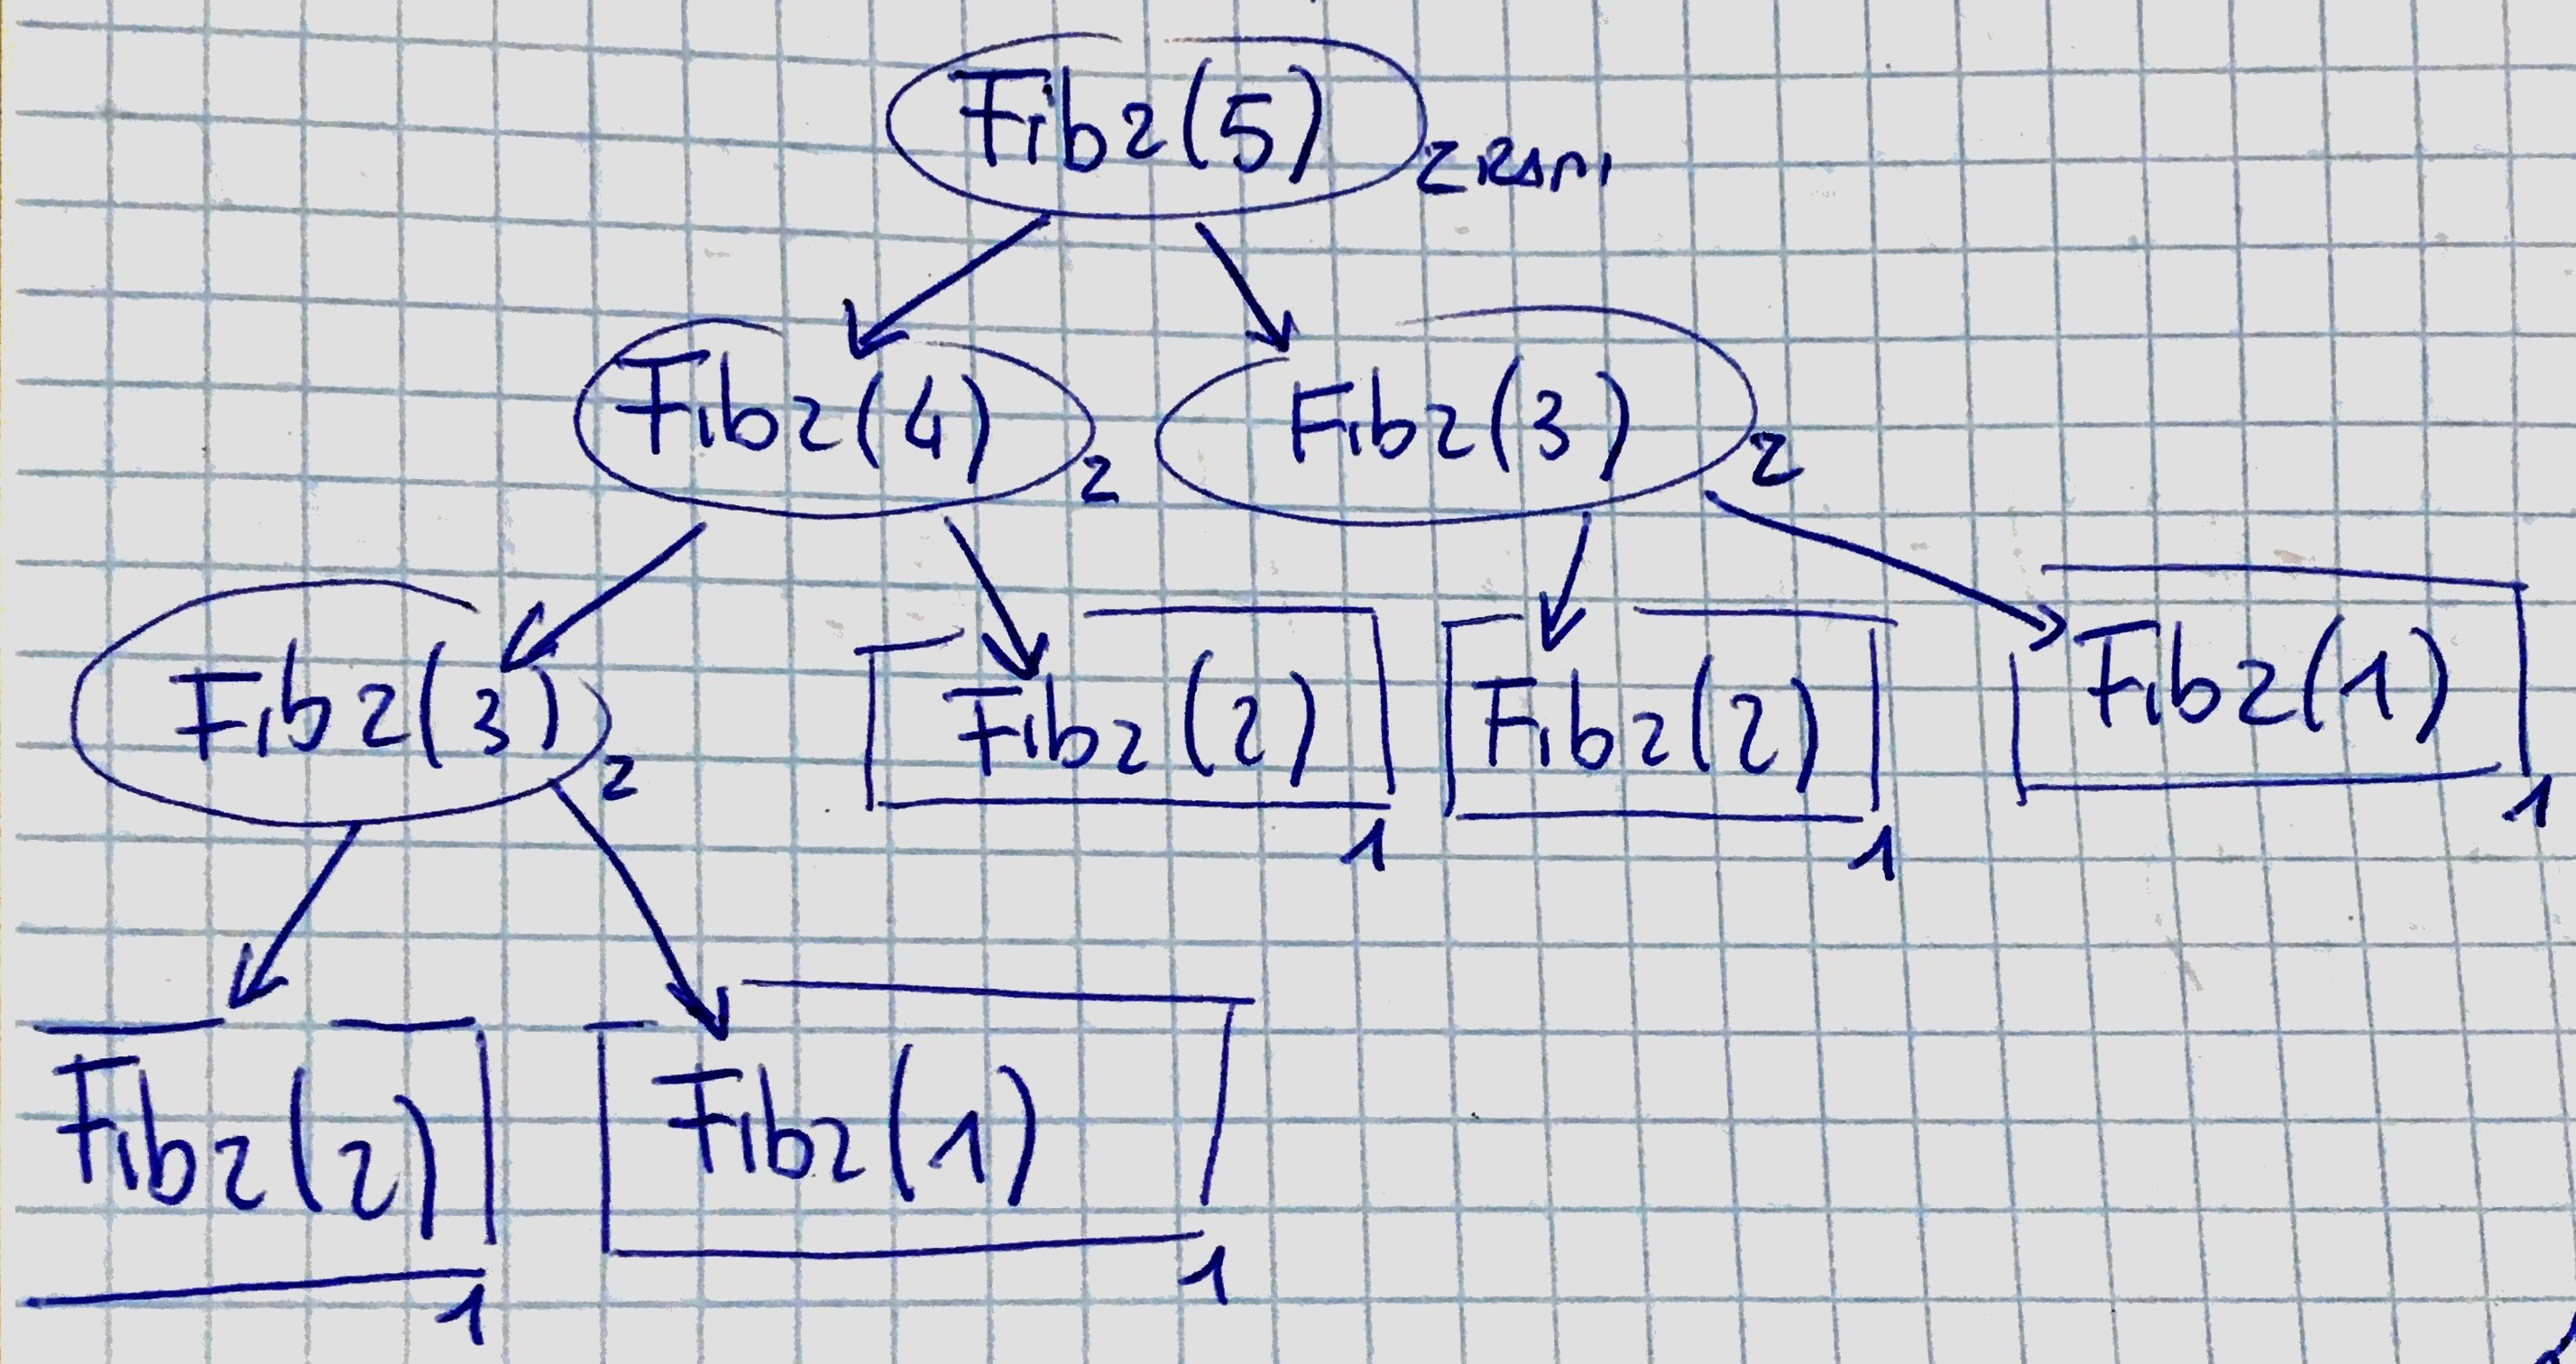
\includegraphics[width=0.5\linewidth]{images/albero-di-chiamata}
\end{center}
La complessità (\textit{numero di istruzioni in questo caso}) di questo algoritmo con questi parametri è data dalla somma $T(5) = 13$\\\\
Ogni albero, come si vede dall'immagine, ha diversi nodi che si differenziano in
\begin{gather*}
	i(T_n) \qquad \textit{nodi interni}\\
	f(T_n) \qquad \textit{nodi foglia}
\end{gather*}
I \textit{nodi interni} sono quelli non terminali (che hanno altri figli), mentre i \textit{nodi foglia} sono quelli esterni (senza figli). La formula generale per determinare la complessità (numero di istruzioni i questo caso) è:
\[
	T_n = 2\cdot i(T_n) + f(T_n)
\]
Ora dobbiamo capire come determinare quanti sono i nodi foglia e quanti quelli interni, al fine di calcolare la complessità di questo algoritmo. \\\\
Se $T_n$ è l'albero di ricorsione di $Fibonaccdi(2)$,allora
\[
	f(T_n) = F_n
\]
Dimostriamo ora per induzione. La base è $n=1,2$ la cui dimostrazione è ovvia. Procedo con il passo induttivo,  per $n\geq 3$:
\begin{center}
	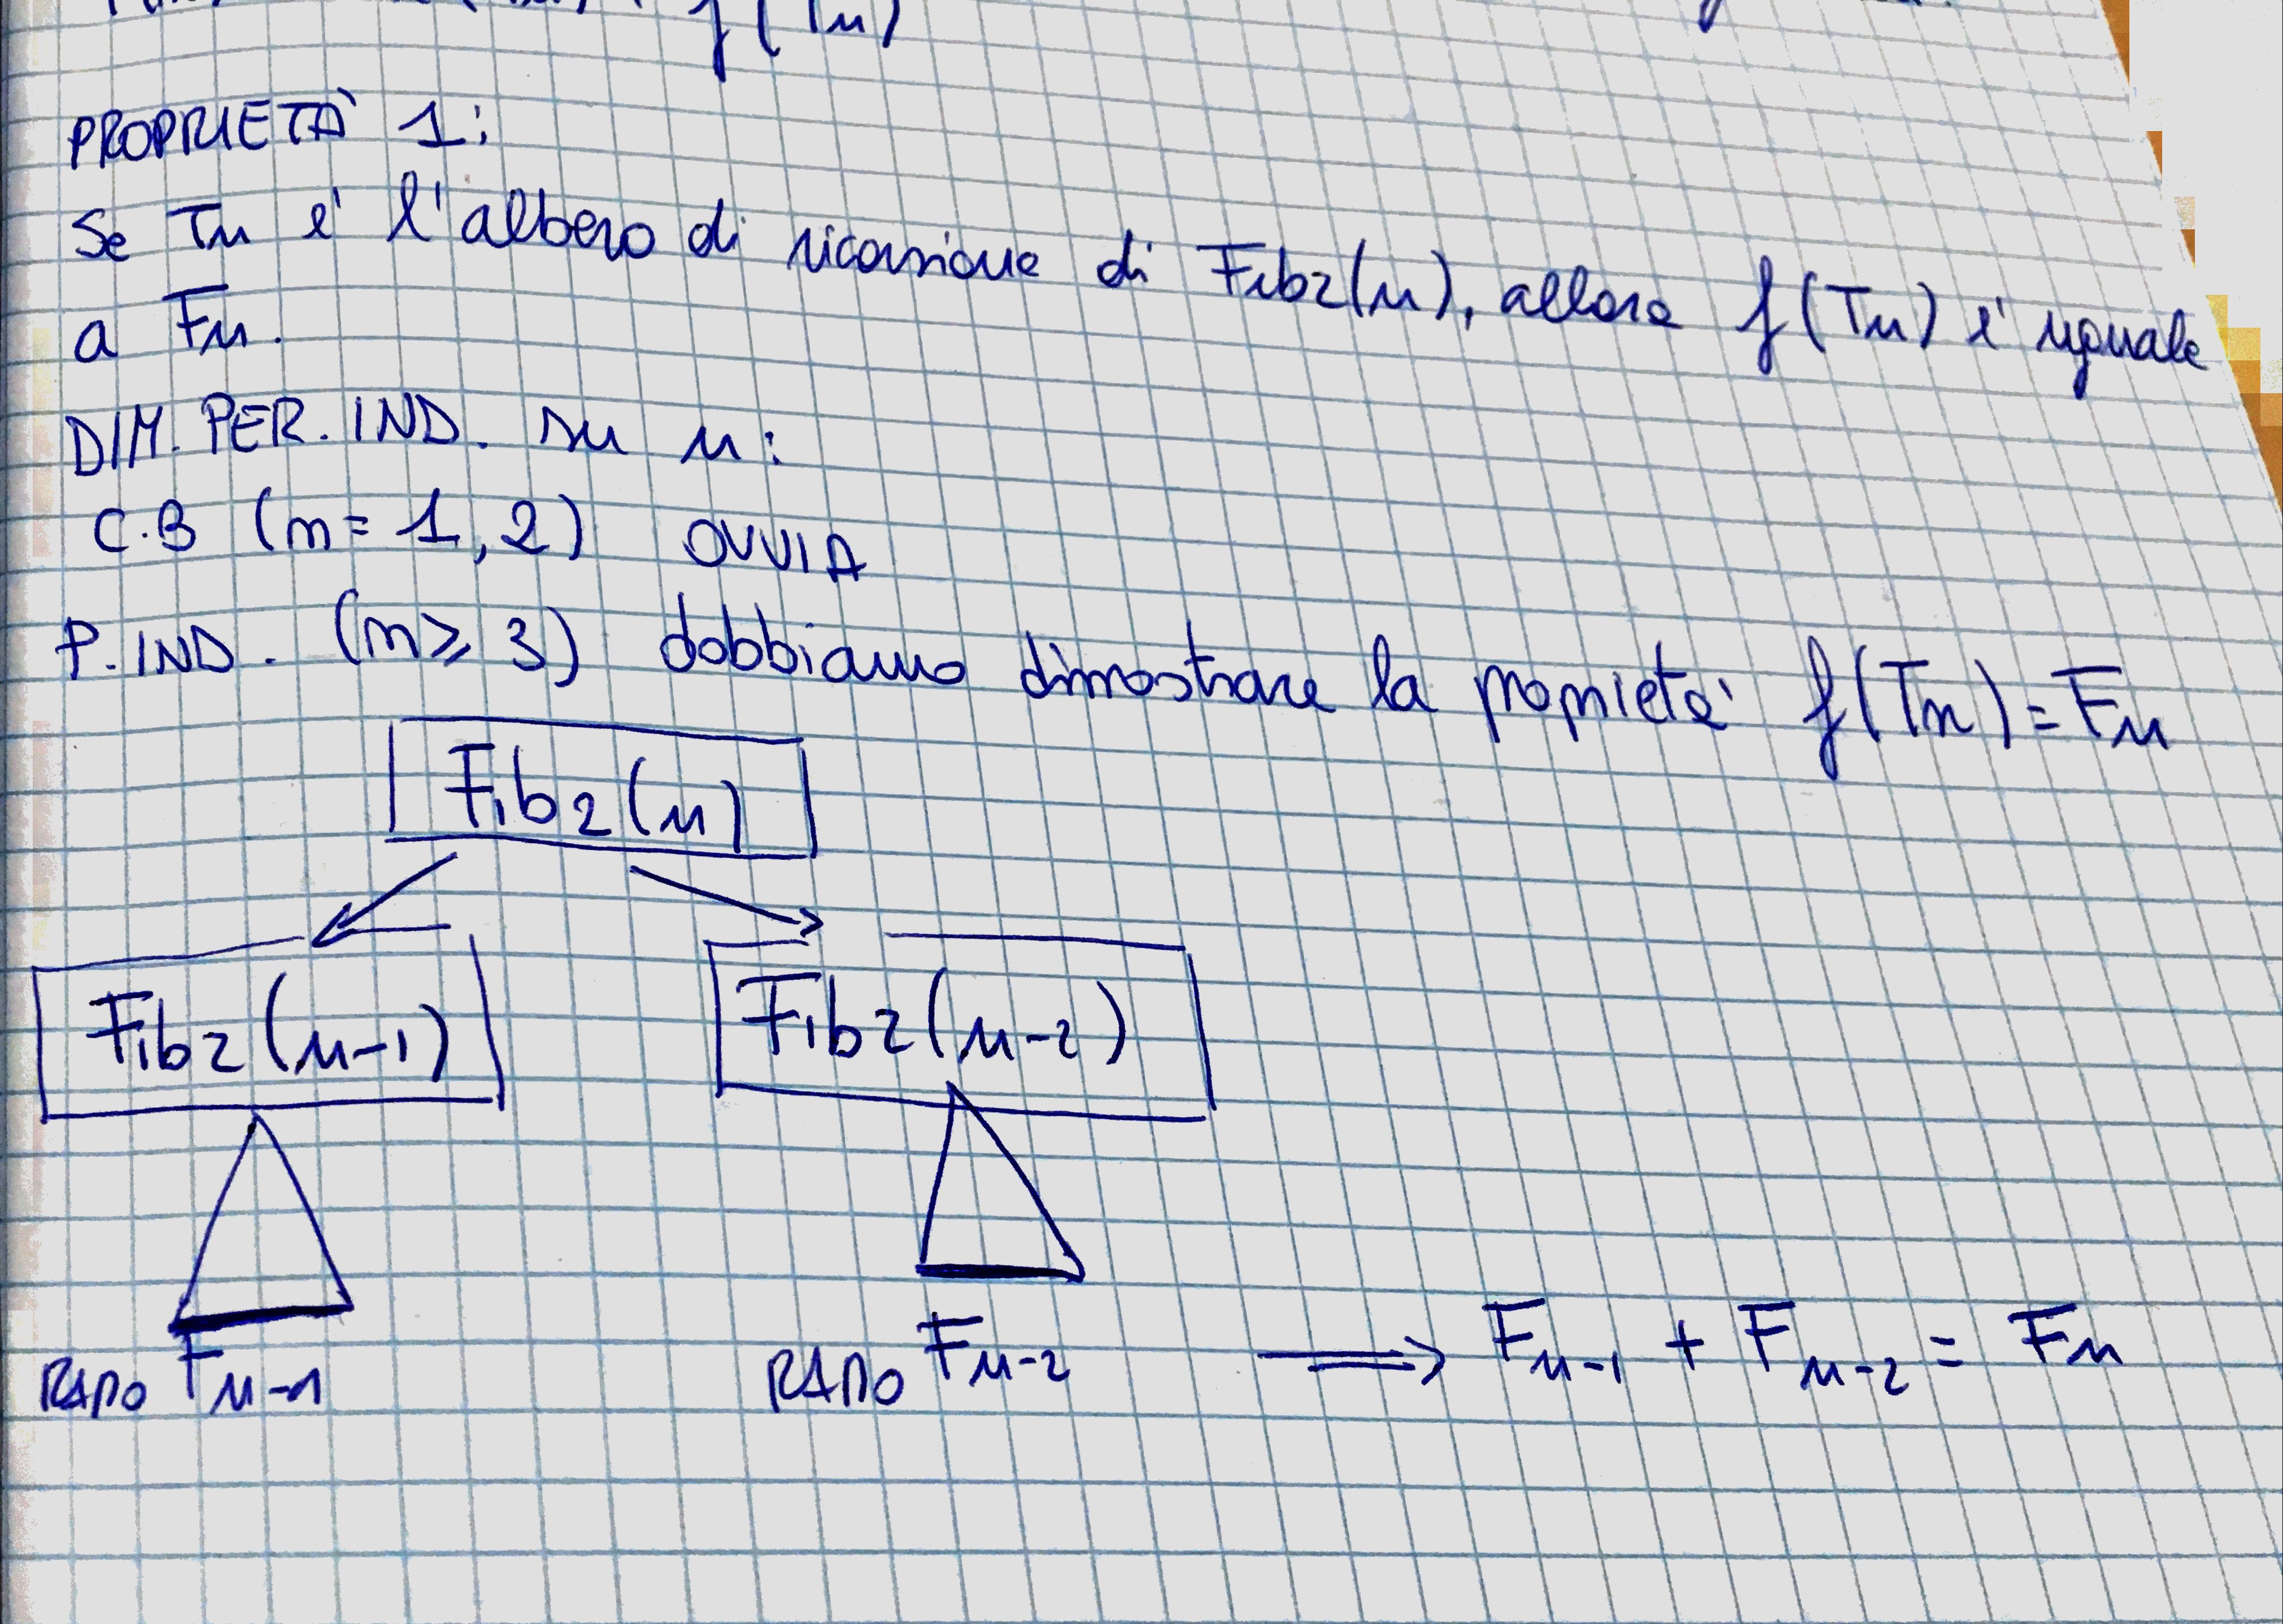
\includegraphics[width=0.5\linewidth]{images/induzione-fibonacci}
\end{center}
quindi $F_{n-1} + F_{n-2} = F_n$.
\pagebreak
\subsubsection{Albero binario}
Se $T$ è un albero binario (dove ogni nodo interno ha esattamente 2 figli), allora $i(T) = f(T) - 1$. Dimostrazione per induzione su $n=$ numero di vertici. Procedo con il test sul caso base con $n=1$, la cui soluzione è ovvia. Applico il passo induttivo: suppongo di avere un albero con il numero di vertici $n \geq 2$ e ipotizzo che la regola precedentemente determinata sia vera fino a $n-1$.
\begin{center}
	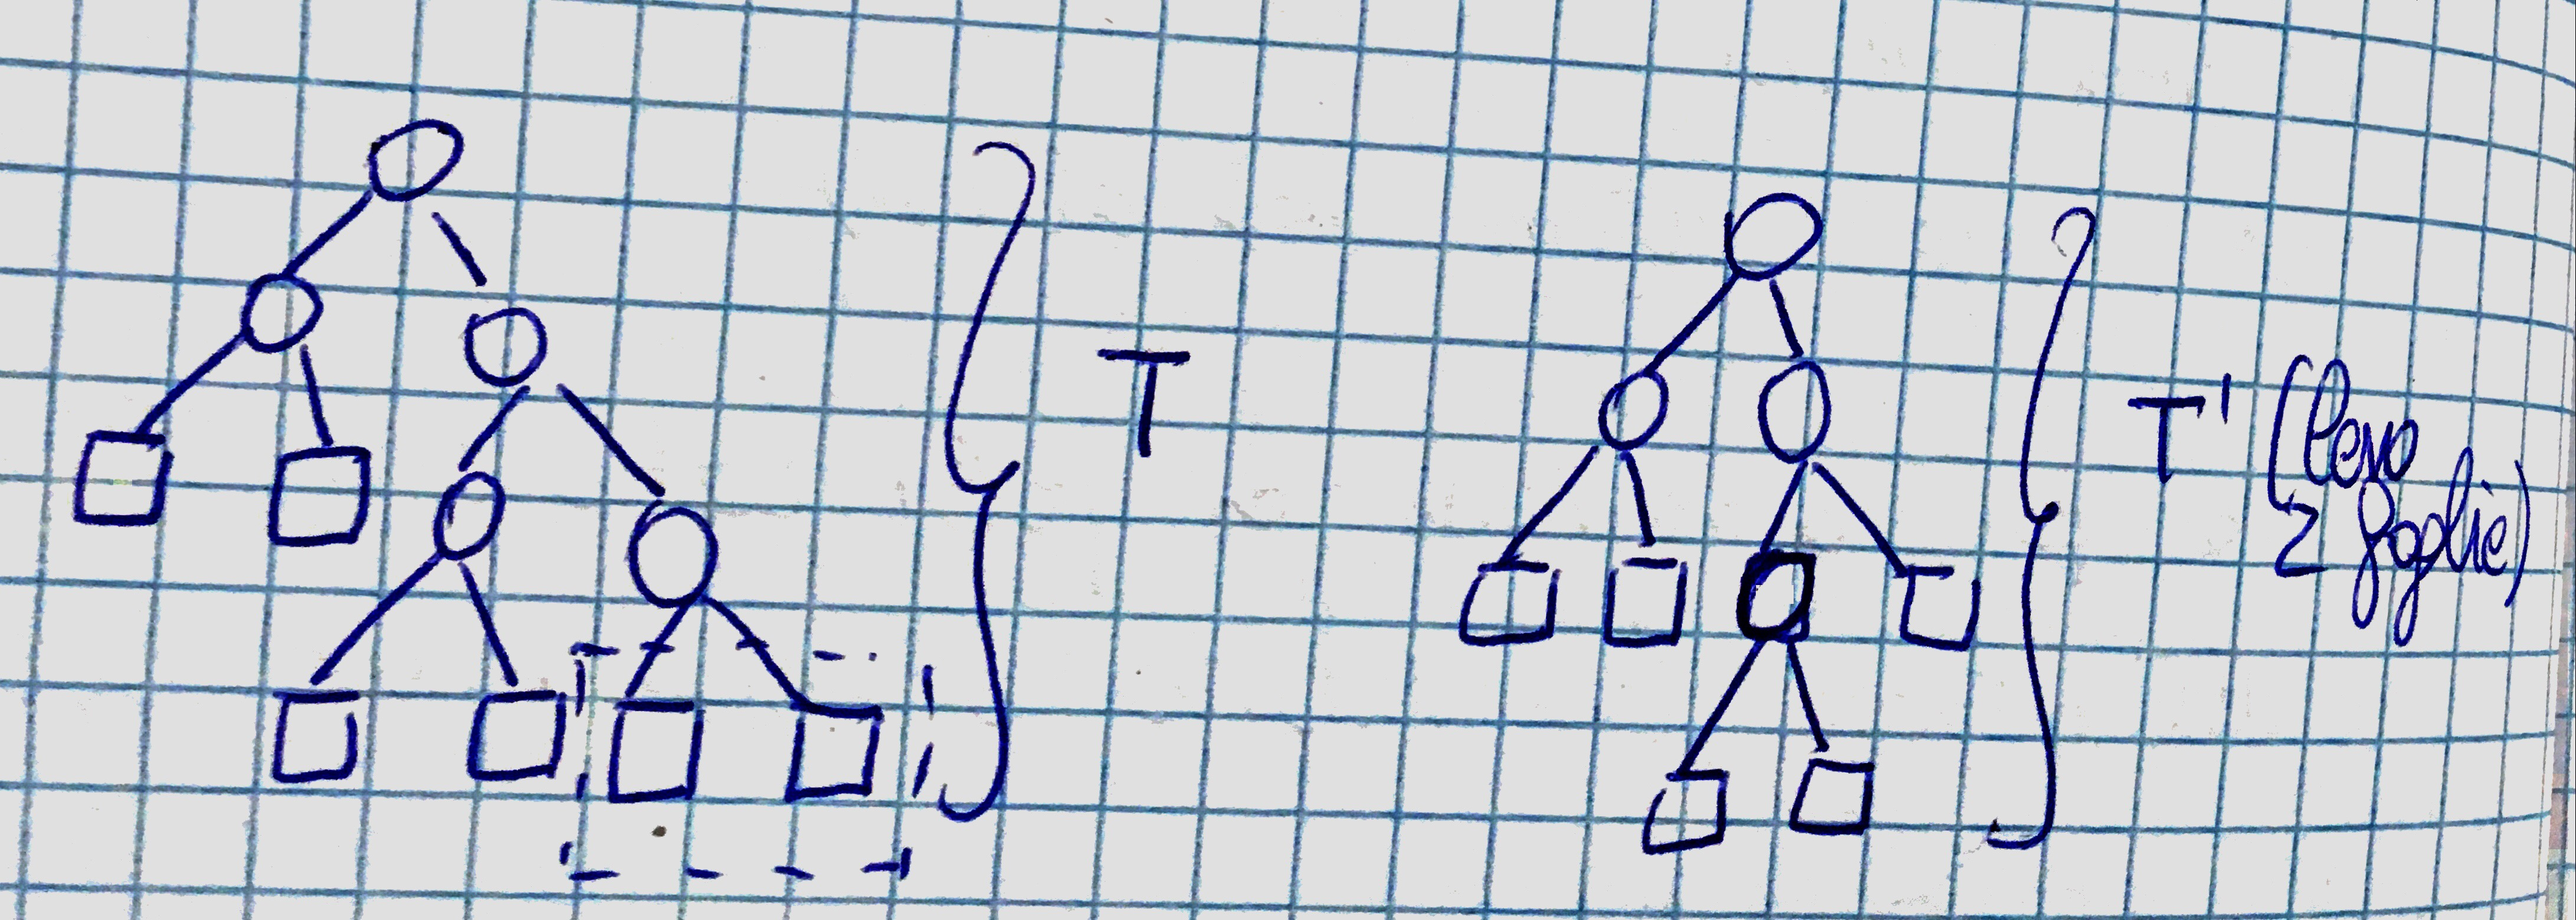
\includegraphics[width=0.5\linewidth]{images/induzione-albero-binario}
\end{center}

Tolgo due foglie dall'albero $T$, e costruisco l'albero $T'$:
\[
	\begin{cases*}
		n(T') = n(T) - 2 \qquad \textit{dove $n(T)$ è il numero di vertici dell'albero $T$}\\
		f(T') = f(T)-1 \qquad \textit{rimuovo 2 foglie, ma il padre di queste due diventa anch'esso foglia}\\
		i(T') = i(T) - 1
	\end{cases*}
\]
allora 
\begin{gather*}
	i(T) = i(T') + 1 \\
	i(T') = f(T') - 1 \\
	i(T) = f(T') \\
	i(T) = f(T)-1
\end{gather*}
Riassumendo, la classe di questo algoritmo ricorsivo è
\begin{gather*}
	T(n) = 2\cdot i(F_n) + f(T_n) = 2(F_n - 1) + F_n = 3F_n - 2 \approx F_n
\end{gather*}
che risulta equivalente ad una classe esponenziale.

\subsection*{Classi di complessità}
Le classi di complessità di un algoritmo più comuni sono 
\begin{gather*}
T_{n} = 2^n \qquad \textit{esponenziale}\\
T_{n} = n^2 \qquad \textit{quadratico}\\
T_{n} = \log_n \qquad \textit{logaritmico}
\end{gather*}

\subsection*{\homeExercize}
Dimostrare per induzione che
\[
	\forall n \geq 6 , F_n \geq 2^{\nicefrac{n}{2}}
\]
Procedo con l'induzione su $n$, calcolando il caso base $n=6$ e $n=7$, in quanto \textit{Fibonacci} ha due casi base.
\begin{gather*}
	F(6) = 8 \geq 2^{\nicefrac{6}{2}} = 2^3 = 8 \checkmark \\
	F(7) = 13 \geq 2^{\nicefrac{7}{2}} \approx 11.3 \checkmark
\end{gather*}
a questo punto applico il passo induttivo per $n \geq 8$:
\begin{gather*}
	\begin{align*}
		F_n &= F_{n-1} + F_{n-2} \\
		 &\geq 2^{\frac{n-1}{2}} + 2^{\frac{n-2}{2}} = 2^{\frac{n}{2} - \frac{1}{2}} + 2^{\frac{n}{2} - 1} = 2^{\frac{n}{2}} \left( 2^{-\frac{1}{2}} + 2^{-1} \right) = 2^{\frac{n}{2}} \underbracket{\left( \frac{1}{\sqrt{2}} + \frac{1}{2}\right)}_{>1} \geq 2^{\frac{n}{2}} \checkmark
	\end{align*}
\end{gather*}
\subsection{Algoritmo iterativo 1}
Al posto di utilizzare un algoritmo ricorsivo, molto elegante ma poco efficiente, provo a riscrivere l'algoritmo di \textit{Fibonacci} utilizzando un algoritmo iterativo:
\begin{lstlisting}[language=c]
	Fibonacci(int n){
		int[n] F;
		F[1] = F[2] = 1;
		for(i=3;i<n;i++){
			F[i] = F[i-1] + F[i-2];
		}
		return F[n];
	}
\end{lstlisting}
\subsection*{\homeExercize}
Determinare la complessità della versione iterativa dell'algoritmo di \textit{Fibonacci}.\\\\
Il numero di istruzioni che vengono eseguite in questa implementazione sono 3 + n° \textit{istruzioni ciclo for}.\\\\
Il numero di istruzioni eseguite in un ciclo \textit{for(i=k to k)} sono: 
\begin{gather*}
	n-k+1 \qquad \text{le volte in cui il corpo del ciclo viene eseguito} \\
	n-k+2 \qquad \text{le volte in cui il test del ciclo viene eseguito}
\end{gather*}
Quindi vengono eseguite $3+(n-2)+(n-1) = 2n$ istruzioni. La classe di appartenenza è quindi \textit{lineare}.

\subsection{Algoritmo iterativo 2}
Al posto di utilizzare l'algoritmo iterativo precedente, che utilizza un array, consideriamo un variante che utilizza 3 variabili in sostituzione dell'array:
\begin{lstlisting}[language=c]
Fibonacci(int n){
	int a=1,b=1,c;
	for(i=3;i<n;i++){
		c=a+b;
		a=b;
		b=c;
	}
	return c;
}
\end{lstlisting}
Riassumendo quindi i diversi algoritmi, possiamo definire la tabella seguente:
\begin{table}[h]
	\centering
	\begin{tabular}{|c|c|c|c|}
		\hline
		& \textbf{$T_n$} & \textbf{Correttezza} & \textbf{Memoria}    \\ \hline
		Fibonacci Binet       & costante       & NO                   & costante            \\ \hline
		Fibonacci ricorsivo   & $\approx 2^n$  & SI                   & lineare $\approx n$ \\ \hline
		Fibonacci iterativo 1 & $\approx n$    & SI                   & lineare $n$         \\ \hline
		Fibonacci iterativo 2 & $\approx n$    & SI                   & costante            \\ \hline
	\end{tabular}
\end{table}
\pagebreak
\section{Notazione asintotica}
Ci sono diverse famiglie di algoritmi.
\begin{enumerate}[itemsep=0mm]
	\item $\varOmicron \to $  o grande
	\item $\varOmega \to$ omega grande
	\item $\varTheta \to$ theta
	\item $\omicron \to$ o piccola
	\item $\omega \to$ omega piccola
\end{enumerate}
\subsection{Definizione di O grande}
Una funzione $f(n)$ appartiene alla classe $\varOmicronClass$ quando
\[
	f(n) \in \varOmicron\left(g(n)\right) \iff \exists c>0 \exists n_0 \in \ins{N} \taleche \forall n \geq n_0 : f(n) \leq c\cdot g(n)
\]
in pratica quando dopo un certo valore $n_0$, $\fn$ tenderà ad $\infty$ meno velocemente di $\gn$.
\subsection{Definizione di Omega grande}
Una funzione $f(n)$ appartiene alla classe $\varOmegaClass$ quando
\[
	f(n) \in \varOmega\left(g(n)\right) \iff \exists c>0 \exists n_0 \in \ins{N} \taleche \forall n \geq n_0 : c\cdot g(n) \leq f(n)
\]
in pratica quando dopo un certo valore $n_0$, $\fn$ tenderà ad $\infty$ più velocemente di $\gn$.
\subsection{Definizione di Theta}
Una funzione $f(n)$ appartiene a questa classe quando:
\[
	f(n) \in \varTheta\left(g(n)\right) \iff \exists c_1 > 0 \exists c_2 > 0 \exists n_0 \in \ins{N} \taleche \forall n_0 : c_1 \cdot g(n) \leq f(n) \leq c_2 \cdot g(n) 
\]
in pratica quando appartiene sia alla classe $\varOmicron$ che alla classe $\varOmega$, ovvero $\fn$ e $\gn$ tendono a $\infty$ allo stesso modo, senza che una delle due prevalga:
\[
	f(n) = \varTheta\left(g(n)\right) \iff f(n) = \varOmicron(g(n)) \land f(n) = \varOmega(g(n))
\]
\nopagebreak
\begin{center}
\definecolor{ffzzqq}{rgb}{1.,0.6,0.}
\definecolor{qqwuqq}{rgb}{0.,0.39215686274509803,0.}
\definecolor{zzttqq}{rgb}{0.6,0.2,0.}
\definecolor{wwwwww}{rgb}{0.4,0.4,0.4}
\begin{tikzpicture}[line cap=round,line join=round,>=triangle 45,x=0.8cm,y=0.8cm]
\draw[->,color=black] (0.,0.) -- (8.,0.);
\foreach \x in {,1.,2.,3.,4.,5.,6.,7.}
\draw[shift={(\x,0)},color=black] (0pt,2pt) -- (0pt,-2pt) node[below] {\footnotesize $\x$};
\draw[->,color=black] (0.,0.) -- (0.,10.);
\foreach \y in {,1.,2.,3.,4.,5.,6.,7.,8.,9.}
\draw[shift={(0,\y)},color=black] (2pt,0pt) -- (-2pt,0pt) node[left] {\footnotesize $\y$};
\draw[color=black] (0pt,-10pt) node[right] {\footnotesize $0$};
\clip(0.,0.) rectangle (8.,10.);
\draw[line width=1.2pt,color=wwwwww] (0.0,-1.0) -- (0.0,-1.0);
\draw[line width=1.2pt,color=wwwwww] (0.0,-1.0) -- (0.02,-0.9797986599732442);
\draw[line width=1.2pt,color=wwwwww] (0.02,-0.9797986599732442) -- (0.04,-0.9591892258076118);
\draw[line width=1.2pt,color=wwwwww] (0.04,-0.9591892258076118) -- (0.06,-0.9381634534546404);
\draw[line width=1.2pt,color=wwwwww] (0.06,-0.9381634534546404) -- (0.08,-0.9167129323250414);
\draw[line width=1.2pt,color=wwwwww] (0.08,-0.9167129323250414) -- (0.1,-0.8948290819243523);
\draw[line width=1.2pt,color=wwwwww] (0.1,-0.8948290819243523) -- (0.12000000000000001,-0.8725031484206243);
\draw[line width=1.2pt,color=wwwwww] (0.12000000000000001,-0.8725031484206243) -- (0.14,-0.8497262011427726);
\draw[line width=1.2pt,color=wwwwww] (0.14,-0.8497262011427726) -- (0.16,-0.8264891290081897);
\draw[line width=1.2pt,color=wwwwww] (0.16,-0.8264891290081897) -- (0.18,-0.8027826368781898);
\draw[line width=1.2pt,color=wwwwww] (0.18,-0.8027826368781898) -- (0.19999999999999998,-0.7785972418398301);
\draw[line width=1.2pt,color=wwwwww] (0.19999999999999998,-0.7785972418398301) -- (0.21999999999999997,-0.7539232694126192);
\draw[line width=1.2pt,color=wwwwww] (0.21999999999999997,-0.7539232694126192) -- (0.23999999999999996,-0.7287508496785953);
\draw[line width=1.2pt,color=wwwwww] (0.23999999999999996,-0.7287508496785953) -- (0.25999999999999995,-0.7030699133342282);
\draw[line width=1.2pt,color=wwwwww] (0.25999999999999995,-0.7030699133342282) -- (0.27999999999999997,-0.6768701876625631);
\draw[line width=1.2pt,color=wwwwww] (0.27999999999999997,-0.6768701876625631) -- (0.3,-0.650141192423997);
\draw[line width=1.2pt,color=wwwwww] (0.3,-0.650141192423997) -- (0.32,-0.622872235664043);
\draw[line width=1.2pt,color=wwwwww] (0.32,-0.622872235664043) -- (0.34,-0.5950524094364062);
\draw[line width=1.2pt,color=wwwwww] (0.34,-0.5950524094364062) -- (0.36000000000000004,-0.5666705854396596);
\draw[line width=1.2pt,color=wwwwww] (0.36000000000000004,-0.5666705854396596) -- (0.38000000000000006,-0.5377154105657753);
\draw[line width=1.2pt,color=wwwwww] (0.38000000000000006,-0.5377154105657753) -- (0.4000000000000001,-0.5081753023587297);
\draw[line width=1.2pt,color=wwwwww] (0.4000000000000001,-0.5081753023587297) -- (0.4200000000000001,-0.4780384443813661);
\draw[line width=1.2pt,color=wwwwww] (0.4200000000000001,-0.4780384443813661) -- (0.4400000000000001,-0.4472927814886638);
\draw[line width=1.2pt,color=wwwwww] (0.4400000000000001,-0.4472927814886638) -- (0.46000000000000013,-0.41592601500551796);
\draw[line width=1.2pt,color=wwwwww] (0.46000000000000013,-0.41592601500551796) -- (0.48000000000000015,-0.38392559780710633);
\draw[line width=1.2pt,color=wwwwww] (0.48000000000000015,-0.38392559780710633) -- (0.5000000000000001,-0.3512787292998718);
\draw[line width=1.2pt,color=wwwwww] (0.5000000000000001,-0.3512787292998718) -- (0.5200000000000001,-0.3179723503011136);
\draw[line width=1.2pt,color=wwwwww] (0.5200000000000001,-0.3179723503011136) -- (0.5400000000000001,-0.28399313781514124);
\draw[line width=1.2pt,color=wwwwww] (0.5400000000000001,-0.28399313781514124) -- (0.5600000000000002,-0.24932749970389878);
\draw[line width=1.2pt,color=wwwwww] (0.5600000000000002,-0.24932749970389878) -- (0.5800000000000002,-0.21396156924992638);
\draw[line width=1.2pt,color=wwwwww] (0.5800000000000002,-0.21396156924992638) -- (0.6000000000000002,-0.17788119960949067);
\draw[line width=1.2pt,color=wwwwww] (0.6000000000000002,-0.17788119960949067) -- (0.6200000000000002,-0.1410719581536577);
\draw[line width=1.2pt,color=wwwwww] (0.6200000000000002,-0.1410719581536577) -- (0.6400000000000002,-0.10351912069504832);
\draw[line width=1.2pt,color=wwwwww] (0.6400000000000002,-0.10351912069504832) -- (0.6600000000000003,-0.06520766559796809);
\draw[line width=1.2pt,color=wwwwww] (0.6600000000000003,-0.06520766559796809) -- (0.6800000000000003,-0.026122267769551843);
\draw[line width=1.2pt,color=wwwwww] (0.6800000000000003,-0.026122267769551843) -- (0.7000000000000003,0.013752707470477077);
\draw[line width=1.2pt,color=wwwwww] (0.7000000000000003,0.013752707470477077) -- (0.7200000000000003,0.05443321064388851);
\draw[line width=1.2pt,color=wwwwww] (0.7200000000000003,0.05443321064388851) -- (0.7400000000000003,0.09593551449436521);
\draw[line width=1.2pt,color=wwwwww] (0.7400000000000003,0.09593551449436521) -- (0.7600000000000003,0.1382762204968193);
\draw[line width=1.2pt,color=wwwwww] (0.7600000000000003,0.1382762204968193) -- (0.7800000000000004,0.18147226549820195);
\draw[line width=1.2pt,color=wwwwww] (0.7800000000000004,0.18147226549820195) -- (0.8000000000000004,0.22554092849246832);
\draw[line width=1.2pt,color=wwwwww] (0.8000000000000004,0.22554092849246832) -- (0.8200000000000004,0.2704998375324066);
\draw[line width=1.2pt,color=wwwwww] (0.8200000000000004,0.2704998375324066) -- (0.8400000000000004,0.3163669767810924);
\draw[line width=1.2pt,color=wwwwww] (0.8400000000000004,0.3163669767810924) -- (0.8600000000000004,0.36316069370579607);
\draw[line width=1.2pt,color=wwwwww] (0.8600000000000004,0.36316069370579607) -- (0.8800000000000004,0.41089970641721063);
\draw[line width=1.2pt,color=wwwwww] (0.8800000000000004,0.41089970641721063) -- (0.9000000000000005,0.45960311115695074);
\draw[line width=1.2pt,color=wwwwww] (0.9000000000000005,0.45960311115695074) -- (0.9200000000000005,0.5092903899362988);
\draw[line width=1.2pt,color=wwwwww] (0.9200000000000005,0.5092903899362988) -- (0.9400000000000005,0.5599814183292726);
\draw[line width=1.2pt,color=wwwwww] (0.9400000000000005,0.5599814183292726) -- (0.9600000000000005,0.6116964734231187);
\draw[line width=1.2pt,color=wwwwww] (0.9600000000000005,0.6116964734231187) -- (0.9800000000000005,0.6644562419294182);
\draw[line width=1.2pt,color=wwwwww] (0.9800000000000005,0.6644562419294182) -- (1.0000000000000004,0.7182818284590464);
\draw[line width=1.2pt,color=wwwwww] (1.0000000000000004,0.7182818284590464) -- (1.0200000000000005,0.7731947639642991);
\draw[line width=1.2pt,color=wwwwww] (1.0200000000000005,0.7731947639642991) -- (1.0400000000000005,0.8292170143515607);
\draw[line width=1.2pt,color=wwwwww] (1.0400000000000005,0.8292170143515607) -- (1.0600000000000005,0.8863709892679594);
\draw[line width=1.2pt,color=wwwwww] (1.0600000000000005,0.8863709892679594) -- (1.0800000000000005,0.944679551065525);
\draw[line width=1.2pt,color=wwwwww] (1.0800000000000005,0.944679551065525) -- (1.1000000000000005,1.0041660239464347);
\draw[line width=1.2pt,color=wwwwww] (1.1000000000000005,1.0041660239464347) -- (1.1200000000000006,1.0648542032930037);
\draw[line width=1.2pt,color=wwwwww] (1.1200000000000006,1.0648542032930037) -- (1.1400000000000006,1.1267683651861575);
\draw[line width=1.2pt,color=wwwwww] (1.1400000000000006,1.1267683651861575) -- (1.1600000000000006,1.1899332761161863);
\draw[line width=1.2pt,color=wwwwww] (1.1600000000000006,1.1899332761161863) -- (1.1800000000000006,1.2543742028896725);
\draw[line width=1.2pt,color=wwwwww] (1.1800000000000006,1.2543742028896725) -- (1.2000000000000006,1.3201169227365495);
\draw[line width=1.2pt,color=wwwwww] (1.2000000000000006,1.3201169227365495) -- (1.2200000000000006,1.3871877336213365);
\draw[line width=1.2pt,color=wwwwww] (1.2200000000000006,1.3871877336213365) -- (1.2400000000000007,1.4556134647626777);
\draw[line width=1.2pt,color=wwwwww] (1.2400000000000007,1.4556134647626777) -- (1.2600000000000007,1.5254214873653842);
\draw[line width=1.2pt,color=wwwwww] (1.2600000000000007,1.5254214873653842) -- (1.2800000000000007,1.596639725569284);
\draw[line width=1.2pt,color=wwwwww] (1.2800000000000007,1.596639725569284) -- (1.3000000000000007,1.6692966676192467);
\draw[line width=1.2pt,color=wwwwww] (1.3000000000000007,1.6692966676192467) -- (1.3200000000000007,1.7434213772608649);
\draw[line width=1.2pt,color=wwwwww] (1.3200000000000007,1.7434213772608649) -- (1.3400000000000007,1.8190435053663383);
\draw[line width=1.2pt,color=wwwwww] (1.3400000000000007,1.8190435053663383) -- (1.3600000000000008,1.896193301795217);
\draw[line width=1.2pt,color=wwwwww] (1.3600000000000008,1.896193301795217) -- (1.3800000000000008,1.9749016274947508);
\draw[line width=1.2pt,color=wwwwww] (1.3800000000000008,1.9749016274947508) -- (1.4000000000000008,2.055199966844677);
\draw[line width=1.2pt,color=wwwwww] (1.4000000000000008,2.055199966844677) -- (1.4200000000000008,2.1371204402513957);
\draw[line width=1.2pt,color=wwwwww] (1.4200000000000008,2.1371204402513957) -- (1.4400000000000008,2.220695816996556);
\draw[line width=1.2pt,color=wwwwww] (1.4400000000000008,2.220695816996556) -- (1.4600000000000009,2.305959528345209);
\draw[line width=1.2pt,color=wwwwww] (1.4600000000000009,2.305959528345209) -- (1.4800000000000009,2.3929456809187606);
\draw[line width=1.2pt,color=wwwwww] (1.4800000000000009,2.3929456809187606) -- (1.5000000000000009,2.481689070338068);
\draw[line width=1.2pt,color=wwwwww] (1.5000000000000009,2.481689070338068) -- (1.520000000000001,2.5722251951421633);
\draw[line width=1.2pt,color=wwwwww] (1.520000000000001,2.5722251951421633) -- (1.540000000000001,2.66459027098813);
\draw[line width=1.2pt,color=wwwwww] (1.540000000000001,2.66459027098813) -- (1.560000000000001,2.7588212451378578);
\draw[line width=1.2pt,color=wwwwww] (1.560000000000001,2.7588212451378578) -- (1.580000000000001,2.8549558112374376);
\draw[line width=1.2pt,color=wwwwww] (1.580000000000001,2.8549558112374376) -- (1.600000000000001,2.9530324243951194);
\draw[line width=1.2pt,color=wwwwww] (1.600000000000001,2.9530324243951194) -- (1.620000000000001,3.053090316563872);
\draw[line width=1.2pt,color=wwwwww] (1.620000000000001,3.053090316563872) -- (1.640000000000001,3.1551695122346857);
\draw[line width=1.2pt,color=wwwwww] (1.640000000000001,3.1551695122346857) -- (1.660000000000001,3.2593108444469037);
\draw[line width=1.2pt,color=wwwwww] (1.660000000000001,3.2593108444469037) -- (1.680000000000001,3.36555597112198);
\draw[line width=1.2pt,color=wwwwww] (1.680000000000001,3.36555597112198) -- (1.700000000000001,3.4739473917272052);
\draw[line width=1.2pt,color=wwwwww] (1.700000000000001,3.4739473917272052) -- (1.720000000000001,3.58452846427606);
\draw[line width=1.2pt,color=wwwwww] (1.720000000000001,3.58452846427606) -- (1.740000000000001,3.697343422671997);
\draw[line width=1.2pt,color=wwwwww] (1.740000000000001,3.697343422671997) -- (1.7600000000000011,3.812437394402594);
\draw[line width=1.2pt,color=wwwwww] (1.7600000000000011,3.812437394402594) -- (1.7800000000000011,3.929856418591152);
\draw[line width=1.2pt,color=wwwwww] (1.7800000000000011,3.929856418591152) -- (1.8000000000000012,4.049647464412953);
\draw[line width=1.2pt,color=wwwwww] (1.8000000000000012,4.049647464412953) -- (1.8200000000000012,4.17185844988356);
\draw[line width=1.2pt,color=wwwwww] (1.8200000000000012,4.17185844988356) -- (1.8400000000000012,4.296538261026663);
\draw[line width=1.2pt,color=wwwwww] (1.8400000000000012,4.296538261026663) -- (1.8600000000000012,4.423736771429141);
\draw[line width=1.2pt,color=wwwwww] (1.8600000000000012,4.423736771429141) -- (1.8800000000000012,4.553504862191156);
\draw[line width=1.2pt,color=wwwwww] (1.8800000000000012,4.553504862191156) -- (1.9000000000000012,4.685894442279277);
\draw[line width=1.2pt,color=wwwwww] (1.9000000000000012,4.685894442279277) -- (1.9200000000000013,4.820958469290757);
\draw[line width=1.2pt,color=wwwwww] (1.9200000000000013,4.820958469290757) -- (1.9400000000000013,4.95875097063728);
\draw[line width=1.2pt,color=wwwwww] (1.9400000000000013,4.95875097063728) -- (1.9600000000000013,5.099327065156642);
\draw[line width=1.2pt,color=wwwwww] (1.9600000000000013,5.099327065156642) -- (1.9800000000000013,5.242742985161021);
\draw[line width=1.2pt,color=wwwwww] (1.9800000000000013,5.242742985161021) -- (2.0000000000000013,5.389056098930659);
\draw[line width=1.2pt,color=wwwwww] (2.0000000000000013,5.389056098930659) -- (2.0200000000000014,5.538324933661931);
\draw[line width=1.2pt,color=wwwwww] (2.0200000000000014,5.538324933661931) -- (2.0400000000000014,5.690609198879008);
\draw[line width=1.2pt,color=wwwwww] (2.0400000000000014,5.690609198879008) -- (2.0600000000000014,5.845969810318459);
\draw[line width=1.2pt,color=wwwwww] (2.0600000000000014,5.845969810318459) -- (2.0800000000000014,6.004468914296362);
\draw[line width=1.2pt,color=wwwwww] (2.0800000000000014,6.004468914296362) -- (2.1000000000000014,6.166169912567661);
\draw[line width=1.2pt,color=wwwwww] (2.1000000000000014,6.166169912567661) -- (2.1200000000000014,6.331137487687704);
\draw[line width=1.2pt,color=wwwwww] (2.1200000000000014,6.331137487687704) -- (2.1400000000000015,6.499437628886135);
\draw[line width=1.2pt,color=wwwwww] (2.1400000000000015,6.499437628886135) -- (2.1600000000000015,6.671137658463467);
\draw[line width=1.2pt,color=wwwwww] (2.1600000000000015,6.671137658463467) -- (2.1800000000000015,6.846306258720894);
\draw[line width=1.2pt,color=wwwwww] (2.1800000000000015,6.846306258720894) -- (2.2000000000000015,7.025013499434133);
\draw[line width=1.2pt,color=wwwwww] (2.2000000000000015,7.025013499434133) -- (2.2200000000000015,7.207330865882264);
\draw[line width=1.2pt,color=wwwwww] (2.2200000000000015,7.207330865882264) -- (2.2400000000000015,7.3933312874427966);
\draw[line width=1.2pt,color=wwwwww] (2.2400000000000015,7.3933312874427966) -- (2.2600000000000016,7.583089166764392);
\draw[line width=1.2pt,color=wwwwww] (2.2600000000000016,7.583089166764392) -- (2.2800000000000016,7.77668040952892);
\draw[line width=1.2pt,color=wwwwww] (2.2800000000000016,7.77668040952892) -- (2.3000000000000016,7.974182454814736);
\draw[line width=1.2pt,color=wwwwww] (2.3000000000000016,7.974182454814736) -- (2.3200000000000016,8.17567430607335);
\draw[line width=1.2pt,color=wwwwww] (2.3200000000000016,8.17567430607335) -- (2.3400000000000016,8.38123656273186);
\draw[line width=1.2pt,color=wwwwww] (2.3400000000000016,8.38123656273186) -- (2.3600000000000017,8.590951452433798);
\draw[line width=1.2pt,color=wwwwww] (2.3600000000000017,8.590951452433798) -- (2.3800000000000017,8.804902863931275);
\draw[line width=1.2pt,color=wwwwww] (2.3800000000000017,8.804902863931275) -- (2.4000000000000017,9.023176380641619);
\draw[line width=1.2pt,color=wwwwww] (2.4000000000000017,9.023176380641619) -- (2.4200000000000017,9.245859314881864);
\draw[line width=1.2pt,color=wwwwww] (2.4200000000000017,9.245859314881864) -- (2.4400000000000017,9.473040742794852);
\draw[line width=1.2pt,color=wwwwww] (2.4400000000000017,9.473040742794852) -- (2.4600000000000017,9.704811539980874);
\draw[line width=1.2pt,color=wwwwww] (2.4600000000000017,9.704811539980874) -- (2.4800000000000018,9.941264417849123);
\draw[line width=1.2pt,color=wwwwww] (2.4800000000000018,9.941264417849123) -- (2.5000000000000018,10.182493960703493);
\draw[line width=1.2pt,color=wwwwww] (2.5000000000000018,10.182493960703493) -- (2.520000000000002,10.428596663577563);
\draw[line width=1.2pt,color=wwwwww] (2.520000000000002,10.428596663577563) -- (2.540000000000002,10.679670970833897);
\draw[line width=1.2pt,color=wwwwww] (2.540000000000002,10.679670970833897) -- (2.560000000000002,10.935817315543098);
\draw[line width=1.2pt,color=wwwwww] (2.560000000000002,10.935817315543098) -- (2.580000000000002,11.19713815965838);
\draw[line width=1.2pt,color=wwwwww] (2.580000000000002,11.19713815965838) -- (2.600000000000002,11.463738035001713);
\draw[line width=1.2pt,color=wwwwww] (2.600000000000002,11.463738035001713) -- (2.620000000000002,11.735723585077949);
\draw[line width=1.2pt,color=wwwwww] (2.620000000000002,11.735723585077949) -- (2.640000000000002,12.013203607733638);
\draw[line width=1.2pt,color=wwwwww] (2.640000000000002,12.013203607733638) -- (2.660000000000002,12.296289098677626);
\draw[line width=1.2pt,color=wwwwww] (2.660000000000002,12.296289098677626) -- (2.680000000000002,12.585093295880815);
\draw[line width=1.2pt,color=wwwwww] (2.680000000000002,12.585093295880815) -- (2.700000000000002,12.879731724872862);
\draw[line width=1.2pt,color=wwwwww] (2.700000000000002,12.879731724872862) -- (2.720000000000002,13.180322244953924);
\draw[line width=1.2pt,color=wwwwww] (2.720000000000002,13.180322244953924) -- (2.740000000000002,13.486985096339962);
\draw[line width=1.2pt,color=wwwwww] (2.740000000000002,13.486985096339962) -- (2.760000000000002,13.799842948260427);
\draw[line width=1.2pt,color=wwwwww] (2.760000000000002,13.799842948260427) -- (2.780000000000002,14.119020948027575);
\draw[line width=1.2pt,color=wwwwww] (2.780000000000002,14.119020948027575) -- (2.800000000000002,14.44464677109708);
\draw[line width=1.2pt,color=wwwwww] (2.800000000000002,14.44464677109708) -- (2.820000000000002,14.776850672139904);
\draw[line width=1.2pt,color=wwwwww] (2.820000000000002,14.776850672139904) -- (2.840000000000002,15.115765537145911);
\draw[line width=1.2pt,color=wwwwww] (2.840000000000002,15.115765537145911) -- (2.860000000000002,15.461526936580025);
\draw[line width=1.2pt,color=wwwwww] (2.860000000000002,15.461526936580025) -- (2.880000000000002,15.814273179612233);
\draw[line width=1.2pt,color=wwwwww] (2.880000000000002,15.814273179612233) -- (2.900000000000002,16.174145369443096);
\draw[line width=1.2pt,color=wwwwww] (2.900000000000002,16.174145369443096) -- (2.920000000000002,16.541287459746908);
\draw[line width=1.2pt,color=wwwwww] (2.920000000000002,16.541287459746908) -- (2.940000000000002,16.915846312255077);
\draw[line width=1.2pt,color=wwwwww] (2.940000000000002,16.915846312255077) -- (2.960000000000002,17.297971755502797);
\draw[line width=1.2pt,color=wwwwww] (2.960000000000002,17.297971755502797) -- (2.980000000000002,17.68781664476244);
\draw[line width=1.2pt,color=wwwwww] (2.980000000000002,17.68781664476244) -- (3.000000000000002,18.08553692318771);
\draw[line width=1.2pt,color=wwwwww] (3.000000000000002,18.08553692318771) -- (3.0200000000000022,18.491291684192984);
\draw[line width=1.2pt,color=wwwwww] (3.0200000000000022,18.491291684192984) -- (3.0400000000000023,18.9052432350928);
\draw[line width=1.2pt,color=wwwwww] (3.0400000000000023,18.9052432350928) -- (3.0600000000000023,19.327557162026945);
\draw[line width=1.2pt,color=wwwwww] (3.0600000000000023,19.327557162026945) -- (3.0800000000000023,19.758402396197123);
\draw[line width=1.2pt,color=wwwwww] (3.0800000000000023,19.758402396197123) -- (3.1000000000000023,20.197951281441682);
\draw[line width=1.2pt,color=wwwwww] (3.1000000000000023,20.197951281441682) -- (3.1200000000000023,20.646379643175443);
\draw[line width=1.2pt,color=wwwwww] (3.1200000000000023,20.646379643175443) -- (3.1400000000000023,21.103866858722235);
\draw[line width=1.2pt,color=wwwwww] (3.1400000000000023,21.103866858722235) -- (3.1600000000000024,21.570595929068176);
\draw[line width=1.2pt,color=wwwwww] (3.1600000000000024,21.570595929068176) -- (3.1800000000000024,22.046753552064548);
\draw[line width=1.2pt,color=wwwwww] (3.1800000000000024,22.046753552064548) -- (3.2000000000000024,22.532530197109402);
\draw[line width=1.2pt,color=wwwwww] (3.2000000000000024,22.532530197109402) -- (3.2200000000000024,23.028120181337865);
\draw[line width=1.2pt,color=wwwwww] (3.2200000000000024,23.028120181337865) -- (3.2400000000000024,23.53372174735158);
\draw[line width=1.2pt,color=wwwwww] (3.2400000000000024,23.53372174735158) -- (3.2600000000000025,24.0495371425184);
\draw[line width=1.2pt,color=wwwwww] (3.2600000000000025,24.0495371425184) -- (3.2800000000000025,24.57577269987402);
\draw[line width=1.2pt,color=wwwwww] (3.2800000000000025,24.57577269987402) -- (3.3000000000000025,25.11263892065795);
\draw[line width=1.2pt,color=wwwwww] (3.3000000000000025,25.11263892065795) -- (3.3200000000000025,25.660350558516814);
\draw[line width=1.2pt,color=wwwwww] (3.3200000000000025,25.660350558516814) -- (3.3400000000000025,26.21912670540868);
\draw[line width=1.2pt,color=wwwwww] (3.3400000000000025,26.21912670540868) -- (3.3600000000000025,26.789190879242746);
\draw[line width=1.2pt,color=wwwwww] (3.3600000000000025,26.789190879242746) -- (3.3800000000000026,27.370771113289507);
\draw[line width=1.2pt,color=wwwwww] (3.3800000000000026,27.370771113289507) -- (3.4000000000000026,27.964100047397086);
\draw[line width=1.2pt,color=wwwwww] (3.4000000000000026,27.964100047397086) -- (3.4200000000000026,28.569415021050283);
\draw[line width=1.2pt,color=wwwwww] (3.4200000000000026,28.569415021050283) -- (3.4400000000000026,29.186958168309538);
\draw[line width=1.2pt,color=wwwwww] (3.4400000000000026,29.186958168309538) -- (3.4600000000000026,29.81697651466777);
\draw[line width=1.2pt,color=wwwwww] (3.4600000000000026,29.81697651466777) -- (3.4800000000000026,30.45972207586388);
\draw[line width=1.2pt,color=wwwwww] (3.4800000000000026,30.45972207586388) -- (3.5000000000000027,31.115451958692397);
\draw[line width=1.2pt,color=wwwwww] (3.5000000000000027,31.115451958692397) -- (3.5200000000000027,31.784428463849636);
\draw[line width=1.2pt,color=wwwwww] (3.5200000000000027,31.784428463849636) -- (3.5400000000000027,32.466919190857475);
\draw[line width=1.2pt,color=wwwwww] (3.5400000000000027,32.466919190857475) -- (3.5600000000000027,33.1631971451067);
\draw[line width=1.2pt,color=wwwwww] (3.5600000000000027,33.1631971451067) -- (3.5800000000000027,33.87354084706285);
\draw[line width=1.2pt,color=wwwwww] (3.5800000000000027,33.87354084706285) -- (3.6000000000000028,34.59823444367808);
\draw[line width=1.2pt,color=wwwwww] (3.6000000000000028,34.59823444367808) -- (3.6200000000000028,35.33756782205375);
\draw[line width=1.2pt,color=wwwwww] (3.6200000000000028,35.33756782205375) -- (3.640000000000003,36.09183672539911);
\draw[line width=1.2pt,color=wwwwww] (3.640000000000003,36.09183672539911) -- (3.660000000000003,36.86134287133257);
\draw[line width=1.2pt,color=wwwwww] (3.660000000000003,36.86134287133257) -- (3.680000000000003,37.6463940725727);
\draw[line width=1.2pt,color=wwwwww] (3.680000000000003,37.6463940725727) -- (3.700000000000003,38.4473043600675);
\draw[line width=1.2pt,color=wwwwww] (3.700000000000003,38.4473043600675) -- (3.720000000000003,39.26439410861091);
\draw[line width=1.2pt,color=wwwwww] (3.720000000000003,39.26439410861091) -- (3.740000000000003,40.097990164997015);
\draw[line width=1.2pt,color=wwwwww] (3.740000000000003,40.097990164997015) -- (3.760000000000003,40.94842597876314);
\draw[line width=1.2pt,color=wwwwww] (3.760000000000003,40.94842597876314) -- (3.780000000000003,41.81604173557409);
\draw[line width=1.2pt,color=wwwwww] (3.780000000000003,41.81604173557409) -- (3.800000000000003,42.70118449330094);
\draw[line width=1.2pt,color=wwwwww] (3.800000000000003,42.70118449330094) -- (3.820000000000003,43.60420832084886);
\draw[line width=1.2pt,color=wwwwww] (3.820000000000003,43.60420832084886) -- (3.840000000000003,44.525474439789335);
\draw[line width=1.2pt,color=wwwwww] (3.840000000000003,44.525474439789335) -- (3.860000000000003,45.46535136885366);
\draw[line width=1.2pt,color=wwwwww] (3.860000000000003,45.46535136885366) -- (3.880000000000003,46.42421507134531);
\draw[line width=1.2pt,color=wwwwww] (3.880000000000003,46.42421507134531) -- (3.900000000000003,47.402449105530316);
\draw[line width=1.2pt,color=wwwwww] (3.900000000000003,47.402449105530316) -- (3.920000000000003,48.400444778065626);
\draw[line width=1.2pt,color=wwwwww] (3.920000000000003,48.400444778065626) -- (3.940000000000003,49.418601300527065);
\draw[line width=1.2pt,color=wwwwww] (3.940000000000003,49.418601300527065) -- (3.960000000000003,50.4573259490992);
\draw[line width=1.2pt,color=wwwwww] (3.960000000000003,50.4573259490992) -- (3.980000000000003,51.517034227491315);
\draw[line width=1.2pt,color=wwwwww] (3.980000000000003,51.517034227491315) -- (4.000000000000003,52.59815003314437);
\draw[line width=1.2pt,color=wwwwww] (4.000000000000003,52.59815003314437) -- (4.020000000000002,53.701105826795725);
\draw[line width=1.2pt,color=wwwwww] (4.020000000000002,53.701105826795725) -- (4.040000000000002,54.82634280546911);
\draw[line width=1.2pt,color=wwwwww] (4.040000000000002,54.82634280546911) -- (4.060000000000001,55.97431107895936);
\draw[line width=1.2pt,color=wwwwww] (4.060000000000001,55.97431107895936) -- (4.080000000000001,57.14546984988231);
\draw[line width=1.2pt,color=wwwwww] (4.080000000000001,57.14546984988231) -- (4.1000000000000005,58.340287597361986);
\draw[line width=1.2pt,color=wwwwww] (4.1000000000000005,58.340287597361986) -- (4.12,59.559242264428505);
\draw[line width=1.2pt,color=wwwwww] (4.12,59.559242264428505) -- (4.14,60.80282144920164);
\draw[line width=1.2pt,color=wwwwww] (4.14,60.80282144920164) -- (4.159999999999999,62.07152259993657);
\draw[line width=1.2pt,color=wwwwww] (4.159999999999999,62.07152259993657) -- (4.179999999999999,63.36585321400983);
\draw[line width=1.2pt,color=wwwwww] (4.179999999999999,63.36585321400983) -- (4.199999999999998,64.68633104092503);
\draw[line width=1.2pt,color=wwwwww] (4.199999999999998,64.68633104092503) -- (4.219999999999998,66.03348428941952);
\draw[line width=1.2pt,color=wwwwww] (4.219999999999998,66.03348428941952) -- (4.2399999999999975,67.40785183875501);
\draw[line width=1.2pt,color=wwwwww] (4.2399999999999975,67.40785183875501) -- (4.259999999999997,68.80998345427635);
\draw[line width=1.2pt,color=wwwwww] (4.259999999999997,68.80998345427635) -- (4.279999999999997,70.2404400073251);
\draw[line width=1.2pt,color=wwwwww] (4.279999999999997,70.2404400073251) -- (4.299999999999996,71.6997936995955);
\draw[line width=1.2pt,color=wwwwww] (4.299999999999996,71.6997936995955) -- (4.319999999999996,73.18862829202276);
\draw[line width=1.2pt,color=wwwwww] (4.319999999999996,73.18862829202276) -- (4.339999999999995,74.70753933829523);
\draw[line width=1.2pt,color=wwwwww] (4.339999999999995,74.70753933829523) -- (4.359999999999995,76.25713442308384);
\draw[line width=1.2pt,color=wwwwww] (4.359999999999995,76.25713442308384) -- (4.379999999999995,77.83803340508406);
\draw[line width=1.2pt,color=wwwwww] (4.379999999999995,77.83803340508406) -- (4.399999999999994,79.45086866496762);
\draw[line width=1.2pt,color=wwwwww] (4.399999999999994,79.45086866496762) -- (4.419999999999994,81.09628535834322);
\draw[line width=1.2pt,color=wwwwww] (4.419999999999994,81.09628535834322) -- (4.439999999999993,82.77494167382741);
\draw[line width=1.2pt,color=wwwwww] (4.439999999999993,82.77494167382741) -- (4.459999999999993,84.48750909632875);
\draw[line width=1.2pt,color=wwwwww] (4.459999999999993,84.48750909632875) -- (4.479999999999992,86.23467267565078);
\draw[line width=1.2pt,color=wwwwww] (4.479999999999992,86.23467267565078) -- (4.499999999999992,88.01713130052107);
\draw[line width=1.2pt,color=wwwwww] (4.499999999999992,88.01713130052107) -- (4.519999999999992,89.83559797815599);
\draw[line width=1.2pt,color=wwwwww] (4.519999999999992,89.83559797815599) -- (4.539999999999991,91.69080011947312);
\draw[line width=1.2pt,color=wwwwww] (4.539999999999991,91.69080011947312) -- (4.559999999999991,93.58347983006537);
\draw[line width=1.2pt,color=wwwwww] (4.559999999999991,93.58347983006537) -- (4.57999999999999,95.51439420705303);
\draw[line width=1.2pt,color=wwwwww] (4.57999999999999,95.51439420705303) -- (4.59999999999999,97.48431564193278);
\draw[line width=1.2pt,color=wwwwww] (4.59999999999999,97.48431564193278) -- (4.6199999999999894,99.49403212954452);
\draw[line width=1.2pt,color=wwwwww] (4.6199999999999894,99.49403212954452) -- (4.639999999999989,101.54434758327989);
\draw[line width=1.2pt,color=wwwwww] (4.639999999999989,101.54434758327989) -- (4.659999999999989,103.63608215665826);
\draw[line width=1.2pt,color=wwwwww] (4.659999999999989,103.63608215665826) -- (4.679999999999988,105.77007257139918);
\draw[line width=1.2pt,color=wwwwww] (4.679999999999988,105.77007257139918) -- (4.699999999999988,107.94717245212212);
\draw[line width=1.2pt,color=wwwwww] (4.699999999999988,107.94717245212212) -- (4.719999999999987,110.16825266780775);
\draw[line width=1.2pt,color=wwwwww] (4.719999999999987,110.16825266780775) -- (4.739999999999987,112.43420168015714);
\draw[line width=1.2pt,color=wwwwww] (4.739999999999987,112.43420168015714) -- (4.7599999999999865,114.7459258989883);
\draw[line width=1.2pt,color=wwwwww] (4.7599999999999865,114.7459258989883) -- (4.779999999999986,117.10435004481215);
\draw[line width=1.2pt,color=wwwwww] (4.779999999999986,117.10435004481215) -- (4.799999999999986,119.5104175187331);
\draw[line width=1.2pt,color=wwwwww] (4.799999999999986,119.5104175187331) -- (4.819999999999985,121.96509077982205);
\draw[line width=1.2pt,color=wwwwww] (4.819999999999985,121.96509077982205) -- (4.839999999999985,124.46935173011282);
\draw[line width=1.2pt,color=wwwwww] (4.839999999999985,124.46935173011282) -- (4.859999999999984,127.02420210737617);
\draw[line width=1.2pt,color=wwwwww] (4.859999999999984,127.02420210737617) -- (4.879999999999984,129.63066388582806);
\draw[line width=1.2pt,color=wwwwww] (4.879999999999984,129.63066388582806) -- (4.8999999999999835,132.28977968493322);
\draw[line width=1.2pt,color=wwwwww] (4.8999999999999835,132.28977968493322) -- (4.919999999999983,135.00261318646665);
\draw[line width=1.2pt,color=wwwwww] (4.919999999999983,135.00261318646665) -- (4.939999999999983,137.77024956000048);
\draw[line width=1.2pt,color=wwwwww] (4.939999999999983,137.77024956000048) -- (4.959999999999982,140.5937958969865);
\draw[line width=1.2pt,color=wwwwww] (4.959999999999982,140.5937958969865) -- (4.979999999999982,143.47438165360728);
\draw[line width=1.2pt,color=wwwwww] (4.979999999999982,143.47438165360728) -- (4.999999999999981,146.4131591025738);
\draw[line width=1.2pt,color=wwwwww] (4.999999999999981,146.4131591025738) -- (5.019999999999981,149.41130379404984);
\draw[line width=1.2pt,color=wwwwww] (5.019999999999981,149.41130379404984) -- (5.0399999999999805,152.4700150258878);
\draw[line width=1.2pt,color=wwwwww] (5.0399999999999805,152.4700150258878) -- (5.05999999999998,155.59051632336377);
\draw[line width=1.2pt,color=wwwwww] (5.05999999999998,155.59051632336377) -- (5.07999999999998,158.77405592860399);
\draw[line width=1.2pt,color=wwwwww] (5.07999999999998,158.77405592860399) -- (5.099999999999979,162.0219072998983);
\draw[line width=1.2pt,color=wwwwww] (5.099999999999979,162.0219072998983) -- (5.119999999999979,165.33536962110048);
\draw[line width=1.2pt,color=wwwwww] (5.119999999999979,165.33536962110048) -- (5.139999999999978,168.71576832131913);
\draw[line width=1.2pt,color=wwwwww] (5.139999999999978,168.71576832131913) -- (5.159999999999978,172.1644556051069);
\draw[line width=1.2pt,color=wwwwww] (5.159999999999978,172.1644556051069) -- (5.1799999999999775,175.6828109933604);
\draw[line width=1.2pt,color=wwwwww] (5.1799999999999775,175.6828109933604) -- (5.199999999999977,179.272241875147);
\draw[line width=1.2pt,color=wwwwww] (5.199999999999977,179.272241875147) -- (5.219999999999977,182.93418407067907);
\draw[line width=1.2pt,color=wwwwww] (5.219999999999977,182.93418407067907) -- (5.239999999999976,186.67010240566142);
\draw[line width=1.2pt,color=wwwwww] (5.239999999999976,186.67010240566142) -- (5.259999999999976,190.48149129724095);
\draw[line width=1.2pt,color=wwwwww] (5.259999999999976,190.48149129724095) -- (5.279999999999975,194.36987535179347);
\draw[line width=1.2pt,color=wwwwww] (5.279999999999975,194.36987535179347) -- (5.299999999999975,198.3368099747866);
\draw[line width=1.2pt,color=wwwwww] (5.299999999999975,198.3368099747866) -- (5.3199999999999745,202.38388199296276);
\draw[line width=1.2pt,color=wwwwww] (5.3199999999999745,202.38388199296276) -- (5.339999999999974,206.51271028909085);
\draw[line width=1.2pt,color=wwwwww] (5.339999999999974,206.51271028909085) -- (5.359999999999974,210.7249464495411);
\draw[line width=1.2pt,color=wwwwww] (5.359999999999974,210.7249464495411) -- (5.379999999999973,215.0222754249416);
\draw[line width=1.2pt,color=wwwwww] (5.379999999999973,215.0222754249416) -- (5.399999999999973,219.406416204181);
\draw[line width=1.2pt,color=wwwwww] (5.399999999999973,219.406416204181) -- (5.419999999999972,223.87912250202697);
\draw[line width=1.2pt,color=wwwwww] (5.419999999999972,223.87912250202697) -- (5.439999999999972,228.44218346063556);
\draw[line width=1.2pt,color=wwwwww] (5.439999999999972,228.44218346063556) -- (5.4599999999999715,233.0974243652318);
\draw[line width=1.2pt,color=wwwwww] (5.4599999999999715,233.0974243652318) -- (5.479999999999971,237.84670737424827);
\draw[line width=1.2pt,color=wwwwww] (5.479999999999971,237.84670737424827) -- (5.499999999999971,242.69193226421314);
\draw[line width=1.2pt,color=wwwwww] (5.499999999999971,242.69193226421314) -- (5.51999999999997,247.6350371896863);
\draw[line width=1.2pt,color=wwwwww] (5.51999999999997,247.6350371896863) -- (5.53999999999997,252.67799945854688);
\draw[line width=1.2pt,color=wwwwww] (5.53999999999997,252.67799945854688) -- (5.559999999999969,257.8228363229428);
\draw[line width=1.2pt,color=wwwwww] (5.559999999999969,257.8228363229428) -- (5.579999999999969,263.0716057862186);
\draw[line width=1.2pt,color=wwwwww] (5.579999999999969,263.0716057862186) -- (5.599999999999969,268.42640742614407);
\draw[line width=1.2pt,color=wwwwww] (5.599999999999969,268.42640742614407) -- (5.619999999999968,273.88938323477345);
\draw[line width=1.2pt,color=wwwwww] (5.619999999999968,273.88938323477345) -- (5.639999999999968,279.46271847527095);
\draw[line width=1.2pt,color=wwwwww] (5.639999999999968,279.46271847527095) -- (5.659999999999967,285.1486425560448);
\draw[line width=1.2pt,color=wwwwww] (5.659999999999967,285.1486425560448) -- (5.679999999999967,290.94942992254073);
\draw[line width=1.2pt,color=wwwwww] (5.679999999999967,290.94942992254073) -- (5.699999999999966,296.8674009670501);
\draw[line width=1.2pt,color=wwwwww] (5.699999999999966,296.8674009670501) -- (5.719999999999966,302.90492295689813);
\draw[line width=1.2pt,color=wwwwww] (5.719999999999966,302.90492295689813) -- (5.739999999999966,309.0644109813821);
\draw[line width=1.2pt,color=wwwwww] (5.739999999999966,309.0644109813821) -- (5.759999999999965,315.34832891783935);
\draw[line width=1.2pt,color=wwwwww] (5.759999999999965,315.34832891783935) -- (5.779999999999965,321.75919041723125);
\draw[line width=1.2pt,color=wwwwww] (5.779999999999965,321.75919041723125) -- (5.799999999999964,328.29955990963674);
\draw[line width=1.2pt,color=wwwwww] (5.799999999999964,328.29955990963674) -- (5.819999999999964,334.972053630059);
\draw[line width=1.2pt,color=wwwwww] (5.819999999999964,334.972053630059) -- (5.839999999999963,341.77934066495385);
\draw[line width=1.2pt,color=wwwwww] (5.839999999999963,341.77934066495385) -- (5.859999999999963,348.72414401990034);
\draw[line width=1.2pt,color=wwwwww] (5.859999999999963,348.72414401990034) -- (5.879999999999963,355.80924170883907);
\draw[line width=1.2pt,color=wwwwww] (5.879999999999963,355.80924170883907) -- (5.899999999999962,363.03746786531485);
\draw[line width=1.2pt,color=wwwwww] (5.899999999999962,363.03746786531485) -- (5.919999999999962,370.4117138761679);
\draw[line width=1.2pt,color=wwwwww] (5.919999999999962,370.4117138761679) -- (5.939999999999961,377.93492953812705);
\draw[line width=1.2pt,color=wwwwww] (5.939999999999961,377.93492953812705) -- (5.959999999999961,385.6101242377681);
\draw[line width=1.2pt,color=wwwwww] (5.959999999999961,385.6101242377681) -- (5.9799999999999605,393.44036815530814);
\draw[line width=1.2pt,color=wwwwww] (5.9799999999999605,393.44036815530814) -- (5.99999999999996,401.42879349271885);
\draw[line width=1.2pt,color=wwwwww] (5.99999999999996,401.42879349271885) -- (6.01999999999996,409.578595726649);
\draw[line width=1.2pt,color=wwwwww] (6.01999999999996,409.578595726649) -- (6.039999999999959,417.89303488665746);
\draw[line width=1.2pt,color=wwwwww] (6.039999999999959,417.89303488665746) -- (6.059999999999959,426.3754368592691);
\draw[line width=1.2pt,color=wwwwww] (6.059999999999959,426.3754368592691) -- (6.079999999999958,435.0291947183731);
\draw[line width=1.2pt,color=wwwwww] (6.079999999999958,435.0291947183731) -- (6.099999999999958,443.857770082498);
\draw[line width=1.2pt,color=wwwwww] (6.099999999999958,443.857770082498) -- (6.1199999999999575,452.8646944995055);
\draw[line width=1.2pt,color=wwwwww] (6.1199999999999575,452.8646944995055) -- (6.139999999999957,462.0535708592562);
\draw[line width=1.2pt,color=wwwwww] (6.139999999999957,462.0535708592562) -- (6.159999999999957,471.428074834814);
\draw[line width=1.2pt,color=wwwwww] (6.159999999999957,471.428074834814) -- (6.179999999999956,480.9919563527643);
\draw[line width=1.2pt,color=wwwwww] (6.179999999999956,480.9919563527643) -- (6.199999999999956,490.7490410932343);
\draw[line width=1.2pt,color=wwwwww] (6.199999999999956,490.7490410932343) -- (6.219999999999955,500.7032320202164);
\draw[line width=1.2pt,color=zzttqq,smooth,samples=100,domain=0.0:8.0] plot(\x,{(\x)^(1.0/2.0)+(\x)/2.0});
\draw[line width=1.2pt,color=qqwuqq,smooth,samples=100,domain=0.1:8.0] plot(\x,{2.0*ln((\x))});
\draw (0.5,5) node[anchor=north west] {$\varOmega(g(x))$};
\draw[line width=1.2pt,color=ffzzqq,smooth,samples=100,domain=0.0:8.0] plot(\x,{(\x)^(1.0/2.0)+(\x)/2.0+sin((5.0*(\x))*180/pi)});
\draw (6.5,3.5) node[anchor=north west] {$O(g(x))$};
\draw (6.5,5.3) node[anchor=north west] {$\varTheta(g(x))$};
\draw (0.4,2) node[anchor=north west] {$f(x)$};
\end{tikzpicture}
\end{center}


\subsubsection{Dimostrazione}
La sintassi $f(n) = \varOmicron(g(n))$ indica che $f(n)$ appartiene alla classe $\varOmicron(g(n))$. Volendo rappresentare le classi come insiemi, possiamo definire:
\[
	\varThetaClass = \varOmegaClass \cap \varOmicronClass
\]
quindi esprimendolo in funzione di $f(n)$:
\[
	f(n) = \varThetaClass \iff f(n) = \varOmegaClass \land \varOmicronClass
\]
volendolo dimostrare, assumo sia vero che
\begin{gather*}
	f(n) = \varOmicronClass \\
	f(n) = \varOmegaClass
\end{gather*}
e procedo con la dimostrazione della tesi
\[
	f(n) = \varThetaClass
\]
Ora esprimo in forma completa la mia ipotesi:
\begin{gather*}
		\fn = \varOmicronClass = \exists c' > 0 \exists n_0' \in \ins{N} \taleche \forall n \geq n_0' : \fn \leq c' \cdot \gn \\
		\fn = \varOmicronClass = \exists c'' > 0 \exists n_0'' \in \ins{N} \taleche \forall n \geq n_0'' : c'' \cdot \gn \leq \fn
\end{gather*}
e anche la mia tesi
\[
	\fn = \varThetaClass = \exists c_1 > 0 \exists c_2 > 0 \exists n_0 \in \ins{N} \taleche \forall n : c_1 \cdot \gn \leq \fn \leq c_2 \cdot \gn
\]
Sostituisco ora $c_2 = c'$ e $c_1 = c''$. Per far si che la tesia sia valida devo prendere in considerazione un valore che soddifi entrame le equazioni dell'ipotesi, ovvero $n_0 = max(n_0',n_0'')$.
\subsubsection{Esempi}
\paragraph{Esempio 1}
Verificare che
\[
	\sqrt{n+10} = \varTheta(\sqrt{n})
\]
Imposto la formula
\begin{gather*}
	\begin{align*}
		\exists c_1 > 0 \exists c_2 > 0 \exists n_0 \in \ins{N} \taleche \forall n > n_0 &: c_1 \cdot g(n) \leq f(n) \leq c_2 \cdot g(n)\\
																					 &: c_1 \cdot \sqrt{n} \leq \sqrt{n+10} \leq c_2 \cdot \sqrt{n} 
	\end{align*}
\end{gather*}
e inizio a calcolare l aprima parte $c_1 \cdot \sqrt{n} \leq \sqrt{n+10}$:
\[
	c_1 \cdot \sqrt{n} \leq \sqrt{n+10} \iff c_1^2 \cdot n \leq n+10 \iff (c_1^2 - 1)n \leq 10
\]
da cui impongo $c_1^2 - 1 \leq 0 \iff c_1 \leq 1$. Scelgo arbitrariamente $c_1 = 1$ e ricavo $n_0 = 1$. Procedo ora a calcolare la seconda parte, $\sqrt{n+10} \leq c_2 \cdot \sqrt{n}$:
\[
	\sqrt{n+10} \leq c_2\cdot \sqrt{n} \iff n+10 \leq c_2^2 \cdot n \iff 10 \leq n(c_2^2 -1)	
\]
impongo $c_2^2-1 > 0$ da cui ricavo $c_2^2 > 1 \iff c_2 > 1$. Ora posso calolare $n_0 \geq \dfrac{10}{c_2^2-1}$. Arbitrariamente imposto $c_2 = \sqrt{2}$ (che è $>1$), ricavando $n_0 = 10$.

\paragraph{Esempio 2}
Verificare che 
\[
	log(n) = \varOmicronClass
\]
Traccio un grafico delle due funzioni
\begin{center}
\definecolor{zzttff}{rgb}{0.6,0.2,1.}
\tikzpicture[line cap=round,line join=round,>=triangle 45,x=1.0cm,y=1.0cm]
\draw[->,color=black] (-3.,0.) -- (5.,0.);
\foreach \x in {-3,-2,-1,1,2,3,4}
\draw[shift={(\x,0)},color=black] (0pt,2pt) -- (0pt,-2pt) node[below] {$\x$};
\draw[->,color=black] (0.,-2.) -- (0.,3.);
\foreach \y in {-2,-1,1,2}
\draw[shift={(0,\y)},color=black] (2pt,0pt) -- (-2pt,0pt) node[left] {$\y$};
\draw[color=black] (0pt,-10pt) node[right] {$0$};
\clip(-3.,-2.) rectangle (5.,3.);
\draw[line width=1.2pt,color=zzttff,smooth,samples=100,domain=0.1:5.0] plot(\x,{ln((\x))});
\draw [domain=-3.:5.] plot(\x,{(-0.--1.*\x)/1.});
\draw (0.5,-0.5) node[anchor=north west] {$y = \log \left( n \right)$};
\draw (0.2,1.5) node[anchor=north west] {$y =  n$};
\draw[color=zzttff] (0.14646916877202582,-4.075645577131859) node {$f$};
\draw[color=black] (-3.986334387006025,-4.075645577131859) node {$g$};
\endtikzpicture
\end{center}
Possiamo già notare dal grafico che sarà sempre vero.
\pagebreak
\subsection{Proprietà delle classi}
\begin{table}[h]
	\centering
	\begin{tabular}{c|c|c|c|c|}
		\cline{2-5}
													  & \textbf{Riflessiva} & \textbf{Transitiva} & \textbf{Simmetrica} & \textbf{Antisimmetrica} \\ \hline
		\multicolumn{1}{|c|}{$\fn = \varOmicronClass$} & \checkmark          & \checkmark          & \crossmark          &                         \\ \hline
		\multicolumn{1}{|c|}{$\fn = \varOmegaClass$}  & \checkmark          & \checkmark          & \crossmark          &                         \\ \hline
		\multicolumn{1}{|c|}{$\fn = \varThetaClass$}  & \checkmark          & \checkmark          & \checkmark          &                         \\ \hline
	\end{tabular}
\end{table}
\subsection{Definizione di omicron}
\[
	\omicronClass = \{ \fn \;|\; \forall c > 0 \exists n_0 \in \ins{N} \taleche \forall n \geq n_0 : \fn < c\cdot \gn \}
\]
Questa classe è una sotto classe di Omicron:
\[
	\omicronClass \subseteq \varOmicronClass
\]
\subsection{Definizione di omega}
\[
	\omicronClass = \{ \fn \;|\; \forall c > 0 \exists n_0 \in \ins{N} \taleche \forall n \geq n_0 : c\cdot \gn < \fn \}
\]
Questa classe è una sottoclasse di Omega:
\[
	\omicronClass \subseteq \varOmegaClass
\]

\subsection{Esempi}
\subsubsection{Esempio 1}
Determinare se la seguente uguaglianza è vera:
\[
	40n+100 = \varOmicron\left( n^2 + 10n + 300 \right)
\]
Noto intanto che il primo termine è lineare, mentre il secondo è quadratico.
\[
	n^2 - 30n + 200 = 0 \to n_{1,2} = 10,20
\]
da cui ricavo $n_0=20$ e arbitrariamente $c=1$.
\begin{center}
	\definecolor{ffqqqq}{rgb}{1.,0.,0.}
	\definecolor{qqqqff}{rgb}{0.,0.,1.}
	\begin{tikzpicture}[line cap=round,line join=round,>=triangle 45,x=0.1cm,y=0.1cm]
		\draw[->,color=black] (-10.,0.) -- (60.,0.);
		\foreach \x in {-10,10,20,30,40,50}
		\draw[shift={(\x,0)},color=black] (0pt,2pt) -- (0pt,-2pt) node[below] {\footnotesize $\x$};
		\draw[->,color=black] (0.,-10.) -- (0.,60.);
		\foreach \y in {-10,10,20,30,40,50}
		\draw[shift={(0,\y)},color=black] (2pt,0pt) -- (-2pt,0pt) node[left] {\footnotesize $\y$};
		\draw[color=black] (0pt,-10pt) node[right] {\footnotesize $0$};
		\clip(-10.,-10.) rectangle (60.,60.);
		\draw [color=qqqqff,domain=-10.:60.] plot(\x,{(--10.--1.*\x)/1.});
		\draw [samples=50,xshift=50,color=ffqqqq,domain=-40.0:40.0)] plot (\x,{(\x)^2/2/5.0});
		\begin{scriptsize}
			\draw[color=qqqqff] (-25.766959892362706,-16.66752849762975) node {$f$};
		\end{scriptsize}
	\end{tikzpicture}
\end{center}
\subsubsection{Esempio 2}
Determinare se la seguente uguaglianza è vera:
\[
	\underbracket{\dfrac{1}{2}n^2-3n}_{f(n)} = \overbracket{n^2}^{g(n)}
\]
Noto che entrambi i termini sono quadratici. Verifico che esista un $c$ che soddisfi le condizioni della classe $\varOmicron$:
\begin{gather*}
	\dfrac{1}{2}n^2 - 3n \leq c\cdot n^2 \iff \dfrac{1}{2}n -3 \leq c\cdot n = \left( \dfrac{1}{2} - c\right)n \leq 3  
\end{gather*}
da qui capisco che l'uguaglianza è vera $\forall c \geq \dfrac{1}{2}$. Determino $n_0 = 1$ in modo arbitrario, in quanto ininfluente data la precedente imposizione.

\subsubsection{Esempio 3}
Determinare se la seguente uguaglianza è vera:
\[
	\dfrac{1}{2}n^2-3n \geq c\cdot n^2
\]
Noto che entrambi i termini sono quadratici. Verifico che esista un $c$ che soddisfi le condizioni della classe $\varOmega$:
\begin{gather*}
	\dfrac{1}{2}n^2 - 3n \geq c\cdot n^2 = \left( \dfrac{1}{2} -c \right)n \geq 3 = n \geq \dfrac{3}{\frac{1}{2} - c}\iff 
	\dfrac{1}{2} - c > 0 \to c < \dfrac{1}{2} \land c > 0
\end{gather*}
imposto $c=\dfrac{1}{14}$ (\textit{un valore arbitrario dentro al suo range di esistenza}) e procedo al calcolo di $n$:
\begin{gather*}
	n \geq \dfrac{3}{\frac{1}{2} - \frac{1}{14}} = 7
\end{gather*}

\subsubsection{Esempio 4}
Determinare la classe di appartenenza di $f(n)$
\begin{gather*}
	\begin{align*}
		n\sqrt{n} &= 9^{\log_3n} \\
		&= (3^2)^{\log_3n} = 3^{2\log_3n} = 3^{\log_3n^2} = n^2
	\end{align*}
\end{gather*}
da cui ricaviamo che $f(n) = \varOmicron(n^2)$

\subsubsection{Esempio 5}
Determinare se $f(n)$ appartiene o no alla classe
\[
	n! = \varOmicron(n^n)
\]
iniziamo a calcolare $n!$:
\begin{gather*}
	\begin{align*}
		n! &= \overset{\leq n}{1} \cdot \overset{\leq n}{2} \cdot \overset{\leq n}{3} \cdot ... \cdot \overset{\leq n}{n} \\
		&\leq \underbracket{n\cdot n \cdot n \cdot ... \cdot n}_{\text{$n$ volte}}
	\end{align*}
\end{gather*}
da cui ricaviamo che $f(n) = \varOmicron(n^n)$

\subsubsection{Esempio 6}
Determinare se $f(n)$ appartiene o no alla classe
\[
	\log(n!) = \varOmicron(n\log n)
\]
iniziamo a calcolare $\log(n!)$:
\begin{gather*}
\begin{align*}
	\log(n!) &= \log \prod_{i=1}^{n} i \\
	&= \sum_{i=1}^{n} \underbracket{\log i}_{\leq \log(n)} \\
	&\leq n\log(n)
\end{align*}
\end{gather*}
da cui ricaviamo che $f(n) = \varOmicron(n\log n)$
\pagebreak
\subsection{Dimostrazioni con i limiti}
\begin{itemize}
	\item $\fn = \omicronClass$. Se $\fn = \omicronClass$ allora $\fn = \varOmicronClass$, perché $\omicronClass \subseteq \varOmicronClass$:
	\[
		\fn = \omicronClass \iff \lim\limits_{n \to \infty} \dfrac{\fn}{\gn} = 0
	\]
	\item $\fn = \omegaClass$. Se $\fn = \omegaClass$ allora $\fn = \varOmegaClass$, perché $\omegaClass \subseteq \varOmegaClass$:
	\[
		\fn = \omegaClass \iff \lim\limits_{n \to \infty} \dfrac{\fn}{\gn} = \infty
	\]
	\item $\fn = \varThetaClass$:
	\[
	\lim\limits_{n\to\infty} \frac{\fn}{\gn} = L \implies \fn = \varThetaClass
	\]
\end{itemize}
\begin{mdframed}
	\example: verificare che $\fn$ appartenga ad una classe:
	\[
		n = \varOmicron(n\log(\log n)) \to \lim\limits_{n\to\infty} \dfrac{\cancel{n}}{\cancel{n}\log(\log n)} = 0 \qquad\checkmark
	\]
\end{mdframed}
Tuttavia non sempre è possibile utilizzare un limite per determinare l'appartenenza ad una classe. Può infatti accadere che non esista il limite din una funzione, per esempio in casi di funzione oscillante. Esempio:
\[
	(1+\sin n)n = 2n
\]
qui, non potendo applicare il limite in quanto insesistente, dobbiamo impostare:
\begin{gather*}
	\begin{align*}
		\sin n &\leq 1 \\
		1 + \sin n &\leq 1 + 1 = 2 \\
		n(1+\sin n) &\leq 2n
	\end{align*}
\end{gather*}
Andiamo ora ad osservare il grafico:
\begin{center}
	\definecolor{ccqqqq}{rgb}{0.8,0.,0.}
	\definecolor{qqwuqq}{rgb}{0.,0.39215686274509803,0.}
	\begin{tikzpicture}[line cap=round,line join=round,>=triangle 45,x=0.1cm,y=0.1cm]
	\draw[->,color=black] (0,0) -- (50,0);
	\foreach \x in {,10,20,30,40}
	\draw[shift={(\x,0)},color=black] (0pt,2pt) -- (0pt,-2pt) node[below] {\footnotesize $\x$};
	\draw[->,color=black] (0.,0.) -- (0.,60.);
	\foreach \y in {0,10,20,30,40,50}
	\draw[shift={(0,\y)},color=black] (2pt,0pt) -- (-2pt,0pt) node[left] {\footnotesize $\y$};
	\draw[color=black] (0pt,-10pt) node[right] {\footnotesize $0$};
	\clip(0.,0.) rectangle (50.,60.);
	\draw[line width=1.2pt,color=qqwuqq,smooth,samples=100,domain=0.0:50.0] plot(\x,{(1.0+sin(((\x))*180/pi))*(\x)});
	\draw[line width=1.2pt,color=ccqqqq,smooth,samples=100,domain=0.0:50.0] plot(\x,{2.0*(\x)});
	\begin{scriptsize}
	\draw[color=qqwuqq] (13,50) node {$f=(1+\sin n)n$};
	\draw[color=ccqqqq] (13,45) node {$g=2n$};
	\end{scriptsize}
	\end{tikzpicture}
\end{center}
Possiamo concludere affermando che $(1+\sin n)n = \varOmicron(2n)$.
\pagebreak
\begin{mdframed}
	Le diverse classi, semplicisticamente, possono essere viste come:
	\begin{itemize}
		\item $\varOmicron \qquad \leq$
		\item $\varOmega \qquad \geq$
		\item $\varTheta \qquad =$
		\item $\omicron \qquad <$
		\item $\omega \qquad >$
	\end{itemize}	
\end{mdframed}
\homeExercize: verificare che le seguenti funzioni appartengano alle rispettive classi:
\begin{enumerate}[label=\alph*)]
	\item $3n\log n = \varOmicron(5n+\log n^3)$
	\item $2^{n+n} = \varOmicron(2^n)$
	\item $2^n = \varOmega(2^{n+k})$ con $k \in \ins{Z}^+$
\end{enumerate}
\textit{Soluzione a):}
\begin{gather*}
	\lim\limits_{n\to \infty} \dfrac{\fn}{\gn} = \lim\limits_{n\to\infty} \dfrac{3n\log n}{5n+\log n} \overset{l'H\hat{o}pital}{=} \lim\limits_{n\to\infty} \dfrac{3(\log n + 1)}{\frac{3}{n}+5} =  \lim\limits_{n\to\infty} \dfrac{n(\log n + 1)}{5} = +\infty
\end{gather*}
che significa $\fn = \omegaClass$ e quindi $\fn = \varOmegaClass$.
\\\\
\textit{Soluzione b):}
\begin{gather*}
	\begin{align*}
		2^{n+n} &= \underset{\geq 2^n}{2^n} \cdot \underset{\geq 2^n}{2^n} \\
		& > 2^n
	\end{align*}
\end{gather*}
che significa $\fn = \omegaClass$ e quindi $\fn = \varOmegaClass$.\\\\
\exercize: riodinare le seguenti funzione in ordine di crescita asintotica:
\begin{multicols*}{2}
	\begin{enumerate}[label=\alph*)]
		\item $n^2$
		\item $n\log n$
		\item $n^3 + \log n$
		\item $\sqrt{n}$
		\item $n^2+2n\log n$
		\item $\log(\log n)$
		\item $17\log n$
		\item $10n^{\frac{3}{2}}$
		\item $n^5-n^4+2n$
		\item $5n^2\cdot \log(\log n)$
		\item $3n^2+n^3\log n$
		\item $n+6\log n$ 
	\end{enumerate}
	\columnbreak
		\begin{enumerate}[label=\alph*)]
			\item $\log(\log n)$
			\item $17\log n$
			\item $\sqrt{n}$
			\item $n+6\log n$ 
			\item $n\log n$
			\item $10n^{\frac{3}{2}}$
			\item $\{n^2, n^2+2n\log n \}$
			\item $5n^2\cdot \log(\log n)$
			\item $3n^2+n^3\log n$
			\item $n^3 + \log n$
			\item $n^5-n^4+2n$
		\end{enumerate}
\end{multicols*}

\section{Complessità di un algoritmo}
Determinare la complessità(numero di istruzione eseguite) dei seguenti codici. La complessità è espressa nei termini del caso peggiore, ovvero dobbiamo andare a determinare quante istruzioni eseguono queste porzioni di codice nel caso peggiore.
\begin{enumerate}[label=\alph*)]
	\item complessità = $O(T(cond)+max\{ T(blocco1), T(blocco2) \})$
	\begin{lstlisting}[language=c]
	if(cond){
		// blocco 1
	}else{
		// blocco 2
	}
	\end{lstlisting}
	ovvero il numero di istruzioni richieste dalla condizione \textit{cond} e il massimo di istruzioni richieste da uno dei due blocci (teniamo in considerazione in più lungo).
	
	\item complessità = $O(n\cdot T(blocco))$
	\begin{lstlisting}[language=c]
	for(i=1 to n){
		// blocco
	}
	\end{lstlisting}
	ovvero il numero di cicli addizionato al numero di istruzioni eseguite in \textit{blocco}.
	
	\item complessità = $O(n\cdot T(cond) \cdot T(blocco))$
	\begin{lstlisting}[language=c]
	while(cond){
		// blocco
	}
	\end{lstlisting}	
\end{enumerate}
\exercize: analizzare il seguante algoritmo:
\begin{lstlisting}[language=c,mathescape=true]
	ricseq(L : lista, x : item) : boolean {
		foreach(y $\in$ L){
			if(y = x)
				return true;
		}
		return false;
	}
\end{lstlisting}
Calcolaimo i 3 differenti tempi di esecuzione:
\begin{align*}
	&T_{\text{best}}(n) = \varTheta(1) & \text{elemento nella 1° posizione della lista} \\
	&T_{\text{avg}}(n) = \varTheta(\frac{n}{2}) & \text{elemento in media a metà della lista} \\
	&T_{\text{wrost}}(n) = \varTheta(n) & \text{elemento in ultima posizione o non presente nella lista}
\end{align*}
\pagebreak
\subsection{Metodo dell'iterazione}
Dato un algoritmo ricorsivo, dobbiamo cercare di ricondurci ad un algoritmo iterativo. \\\\
\example
\[
	T(n) =
	\begin{cases*}
		c + T(\frac{n}{2}) \qquad \text{con } n=2^k\\
		1
	\end{cases*}
\]
Sviluppo l'algoritmo per cicli, fino a quando non arrivo a riconoscerne lo sviluppo:
\begin{align*}
	T(n) &= c + T(\frac{n}{2}) & \textit{1° ciclo} \\
	&= c + \left[ T(\frac{n}{2^2}) \right] = 2c + T(\frac{n}{2^2}) & \textit{2° ciclo} \\
	&= 2c + \left[ c + T(\frac{n}{2^3}) \right] = 3c + T(\frac{n}{2^3}) &\textit{3° ciclo} \\
	&\;\;\vdots \\
	&= k\cdot c + T(\frac{n}{2^k}) & \frac{n}{2^k} = 1 \iff k = \log n \\
	&= c\cdot \log n + 1
\end{align*}
\example \\
\[
	T(n) =
	\begin{cases*}
		9T(\frac{n}{3}) + n \qquad \text{se } n \geq 2 \\
		1 \qquad \text{se } n=1
	\end{cases*}
\]

\begin{mdframed}
	La serie geometrica $\sum_{i=0}^{k} q^i = \dfrac{q^{k+1}-1}{q-1}$. Se $q=3$ allora $\sum_{i=0}^{k} 3^i = \dfrac{3^{k+1}-1}{2}$.
\end{mdframed}

Inizio a svuluppare per cicli:
\begin{align*}
	T(n) &= 9T(\frac{n}{3}) + n & \textit{1° ciclo} \\
	&= 9\left[ 9T\left(\frac{n}{3^2}\right) + \frac{n}{3} \right] + n = 9^2T \left(\frac{n}{3^2}\right) + 3n + n  & \textit{2° ciclo}\\
	&= 9\left\{ 9 \left[ 9 \left(T \left(\frac{n}{3^3}\right) + \frac{n}{3^2}\right) \right] \right\} + n = 9^3T \left(\frac{n}{3^3}\right) + 9n + 3n + n = 9^3T \left(\frac{n}{3^3}\right) + n(3^2+3^1+3^0)  & \textit{3° ciclo}\\
	&\;\;\vdots \\
	&= 9^k\cdot T(\frac{n}{3^k}) + n\cdot \sum_{i=0}^{k-1} 3^i  & \textit{k° ciclo}\\
	&=  9^k\cdot T(\frac{n}{3^k}) + n\cdot \dfrac{3^k-1}{2} \qquad n=3^k \iff k =\log_3n\\
	&= 9^{\log_3n} + \dfrac{n\cdot 3^{\log_3n}-1}{2} \\
	&= n^2 + \dfrac{n(n-1)}{2} \\
	&= \varOmicron(n^2)
\end{align*}
Sono quindi arrivato a dimostrare che questo algoritmo, riscritto in modalità iterativa, possiede complessità $\varOmicron(n^2)$.

\pagebreak
\subsection{Metodo della sostituzione [p.70]}
\dateright{12 Ottobre 2016}
\example: sapendo che $\lfloor \frac{n}{2} \rfloor$ = il più grande intero inferiore a $\frac{n}{2}$
\[
	T(n) = 
	\begin{cases*}
		1 \qquad \text{se } n=1 \\
		T\left( \lfloor \frac{n}{2} \rfloor \right) + n \qquad \text{se } n \geq 2
	\end{cases*}
\]
devo provare ad indovinare la classe della funzione. Ipotizzo che $T(n) = \varOmicron(n)$. Dimostro per induzione la mia ipotesi:
\[
	\exists c > 0 \taleche T(n) \leq c\cdot n \quad \text{per $n$ sufficientemente grande}
\]
impongo $n_0 = 1$ in modo arbitario, e verifico la base dell'induzione:
\[
	T(1) \leq c\cdot 1 \implies 1 \leq c \implies c \geq 1
\]
ora verifico che valga anche per $n \geq 2$:
\[
	T(n) = 	\underbracket{T\left( \lfloor \frac{n}{2} \rfloor \right)}_{\leq c \lfloor \frac{n}{2} \rfloor} + n \leq c \lfloor \frac{n}{2} \rfloor + n \leq c\frac{n}{2} + n \leq c\frac{n}{2} + n = \left( \frac{c}{2} + 1 \right)n \isLeq c\cdot n
\]
se ora imposto $\frac{c}{2} + 1 \leq c$ e ottengo $c \geq 2$. A questo punto verifico che $c=2$ soddisfi le condizioni iniziali.

\subsection{Teorema master - \textit{metodo dell'esperto} [p.79]}
 \label{sec:masterTheorem}
Questo metodo appartiene alla filosofia \textit{Divide et imperat}. Si suddivide in 3 fasi:
\begin{enumerate}[label=\arabic*)]
	\item Scomposizione del problema
	\item Soluzione dei sottoproblemi
	\item Ricomposizione delle soluzioni dei sottoproblemi
\end{enumerate}
Di conseguenza
\[
	T(n) = T_S(n) + \sum_{i=1}^{k} T(n_i) + T_R(n)
\]
ovvero la complessità dipende da il tempo di scomposizione, dal tempo di soluzione dei $k$ sottoproblemi e infine da il tempo di ricomposizione. Noi indicheremo con $\fn$ la somma tra tempo di scomposizione e ricomposizione. A questo punto
\[
	T(n) = \fn + \sum_{i=1}^{k} T(n_i) 
\]
Il caso di studio che noi andremo a coprire riguarderà solamente le funzioni i cui sottoproblemi hanno medesima dimensione.
\pagebreak
\subsubsection{Definizione}
Siano date le costanti
\begin{gather*}
	a \geq 1 \qquad \text{numero di sottoproblemi} \\
	b > 1 \qquad \text{dimensione originale} 
\end{gather*}
e sia data $\fn$. Sia $T(n)$ una funzione definita come
\[
	T(n) =
	\begin{cases*}
		aT\left( \frac{n}{b} \right) + \fn \\
		1
	\end{cases*}
\]
dove $\frac{n}{b}$ rappresenta la dimensione dei sottoproblemi e $d = log_ba$ è equivalente alla dimensione dell'albero di ricorsione di $T(n)$, allora $T(n)$ può essere asintoticamente limitata nei seguenti modi:
\begin{enumerate}[label=\arabic*)]
	\item Se $\fn = \varOmicron(n^{d-\varepsilon}),\;\varepsilon > 0$ allora $T(n) = \varTheta(n^d)$
	\item Se $\fn = \varTheta(n^{d})$ allora $T(n) = \varTheta(n^d \cdot log(n))$
	\item Se $\fn = \varOmega(n^{d+\varepsilon}),\;\varepsilon > 0\;\exists c<1 \taleche $ per $n$ sufficientemente grande $af(\frac{n}{b}) \leq c\cdot \fn$, allora $T(n) = \varTheta(\fn)$
\end{enumerate}
\paragraph{Esempi}
\subparagraph{\example 1} Determinare la complessità di della funzione $T(n)$ definita come:
\[
	T(n) = c + T\left(\frac{n}{2}\right)
\]
come prima cosa individuo le costanti:
\begin{gather*}
	a = 1 \\
	b = 2
\end{gather*}
e la funzione $\fn = c$. A questo punto determino la dimensione dell'albero di ricorsione:
\[
	d = {log_ba} = log_21 = 0
\]
e trovo $\gn = n^d = n^0 = 1$. Fatto ciò, confronto $\fn$ e $\gn$:
\[
	\fn = \varTheta(\gn)
\]
siamo dunque nel 2° caso, dove $\fn = \varTheta(n^d)$, da cui ricavo:
\[
	T(n) = \varTheta(n^d\cdot \log n) = \varTheta(\log n)
\]
\subparagraph{\example 2} Determinare la complessità di della funzione $T(n)$ definita come:
\[
	T(n) = 3T\left(\frac{n}{2}\right) + n^2
\]
come prima cosa individuo le costanti:
\begin{gather*}
	a = 3 \\
	b = 2
\end{gather*}
e la funzione $\fn = n^2$. A questo punto determino la dimensione dell'albero di ricorsione:
\[
	d = {\log_ba} = \log_23 \approx 1.6
\]
e trovo $\gn = n^d = n^{\log_23}$. Fatto ciò, confronto $\fn$ e $\gn$:
\[
	\fn = \varOmega(\gn)
\]
dal momento che $n^{\log_23} < n^{2+\varepsilon}$ per $\varepsilon < 2 -\log_23$. Siamo dunque nel 3° caso. Verifico ora che $\exists c < 1 \taleche$ per $n$ sufficientemente grande $af(\frac{n}{b}) \leq c\cdot \fn$:
\begin{align*}
	3\left( \frac{n}{2} \right)^2 &\leq c\cdot n^2 \\
	\frac{3}{4}\cancel{n^2} &\leq c\cdot \cancel{n^2} \iff \frac{3}{4} \leq c \leq 1
\end{align*}
provata l'esistenza di $c$, posso concludere che $\fn = \varOmega(n^{d+\varepsilon})$, da cui ricavo (3° caso):
\[
	T(n) = \varTheta(\fn) = \varTheta(n^2)
\]
\subparagraph{\example 3} Determinare la complessità di della funzione $T(n)$ definita come:
\[
	T(n) = 4T\left(\frac{n}{2}\right) + n^2
\]
come prima cosa individuo le costanti:
\begin{gather*}
	a = 4 \\
	b = 2
\end{gather*}
e la funzione $\fn = n^2$. A questo punto determino la dimensione dell'albero di ricorsione:
\[
	d = {log_ba} = log_24 = 2
\]
e trovo $\gn = n^d = n^2$. Fatto ciò, confronto $\fn$ e $\gn$:
\[
	\fn = \varTheta(\gn)
\]
siamo dunque nel 2° caso, dove $\fn = \varTheta(n^d)$, da cui ricavo:
\[
	T(n) = \varTheta(n^d\cdot \log n) = \varTheta(n^2 \cdot\log n)
\]
\subparagraph{\homeExercize 4} Determinare la complessità di della funzione $T(n)$ definita come:
\[
	T(n) = T\left(\frac{n}{2}\right) + 2^n
\]
come prima cosa individuo le costanti:
\begin{gather*}
	a = 1 \\
	b = 2
\end{gather*}
e la funzione $\fn = 2^n$. A questo punto determino la dimensione dell'albero di ricorsione:
\[
	d = {\log_ba} = \log_21 = 0
\]
e trovo $\gn = n^d = n^0 = 1$. Fatto ciò, confronto $\fn$ e $\gn$:
\[
	\fn = \varOmega(\gn)
\]
dal momento che $2^{n+\varepsilon} \geq 1$ per $\varepsilon > 0$ e $n$ sufficentemente grande. Siamo dunque nel 3° caso. Verifico ora che $\exists c < 1 \taleche$ per $n$ sufficientemente grande $af(\frac{n}{b}) \leq c\cdot \fn$:
\begin{align*}
	2^{\frac{n}{2}} &\leq c\cdot 2^n \\
	\nicefrac{2^{\frac{n}{2}}}{2^n} &\leq c \\
	\frac{\cancel{2^n}\cdot2^\frac{1}{2}}{\cancel{2^n}} &\leq c \iff \sqrt{2} \leq c \implies c < 1	
\end{align*}
provata l'esistenza di $c$, posso concludere che $\fn = \varOmega(n^{d+\varepsilon})$, da cui ricavo (3° caso):
\[
	T(n) = \varTheta(\fn) = \varTheta(2^n)
\]
\subsection{Quando non si può applciare}
Il teroema master non si può applicare quando:
\begin{enumerate}[label=\arabic*)]
	\item $a$ non è una costante. 
		\[
			T(n) = \underbracket{2^n}_{\text{non costante}}T(\frac{n}{2}) + n^2
		\]
	\item $\fn$ è negativa. 
		\[
			T(n) = 2T(\frac{n}{2}) - \underbracket{n^2\log n}_{\text{negativa}}
		\]
	\item $a$ non è $\geq 1$. 
		\[
			T(n) = \underbracket{\frac{1}{2}}_{\text{$\not\geq 1$}}T(\frac{n}{2}) + n^3
		\]
\end{enumerate}
\example Determinare la complessità del seguente codice:
\begin{lstlisting}[language=c]
myAlgorithm(int n) : int {
	int a,i,j;
	if(n > 1){
		a=0;
		for(i=0 to n)
			for(j=1 to n)
				a = a + (i+1)*(j+4)	// ripetuto n^2 volte
		for(i=1 to 16)				// per 16 volte richiama con 
			a = a + myAlgorithm(n/4)	// sottoproblemi di 
	}else{						// dimensione n/4
		return n-1;
	}	
}
\end{lstlisting}
Determiniamo $T(n)$:
\[
	T(n) = 
	\begin{cases*}
		n^2 + 16T(\frac{n}{4}) \\
		c
 	\end{cases*}
\]
Trovo 
\begin{gather*}
	a = 16 \\
	b = 4 \\
	f(n) = n^2 \\
	d = \log_416 = 2 \\
	g(n) = n^2 \\
	\fn = \varTheta(\gn) \implies \text{2° caso}\\
	T(n) = \varTheta(n^2 \cdot \log n)
\end{gather*}

\pagebreak
\subsection{Dimostrazione}
\dateright{13 Ottobre 2016}
\begin{center}
	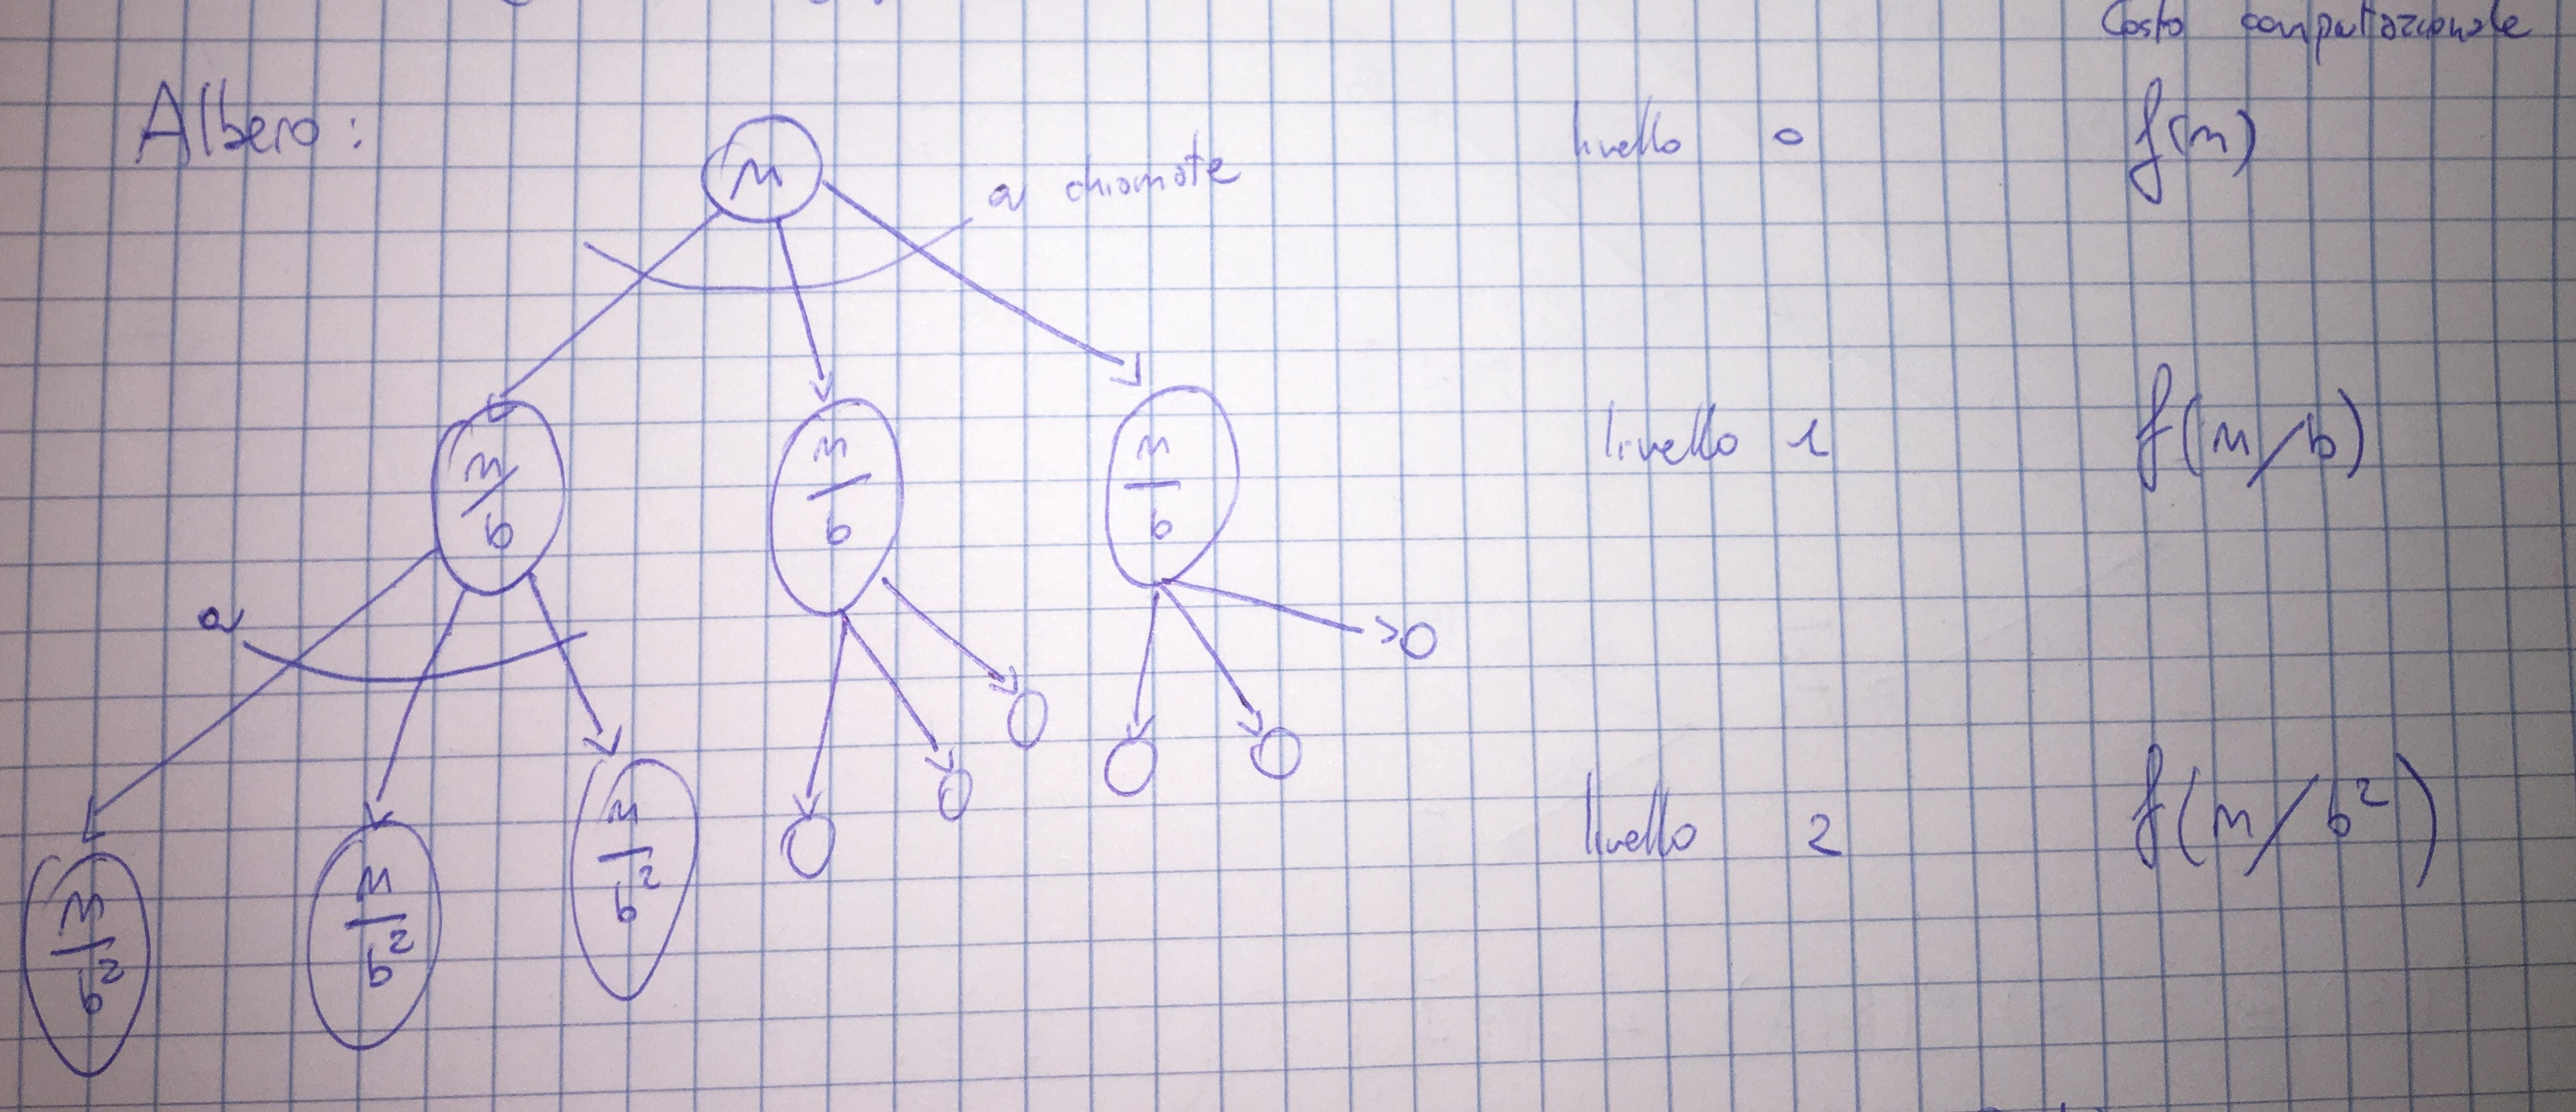
\includegraphics[width=1\linewidth]{images/albero_teorema_master}
\end{center}
\begin{enumerate}[label=\alph*)]
	\item Al livello $i$ la dimensione dei sottoproblemi è $\frac{n}{b^i}$
	\item Al livello $i$ le singole chiamate hanno complessità $f\left(\frac{n}{b^i}\right)$
	\item Al livello $i$, vi saranno $a^i$ vertici
	\item Il numero di livelli dell'albero è $i=\log_bn$
	\item Il numero di foglie è $a^{\log_bn} = n^d$
\end{enumerate}
\pagebreak
\section{Tipo di dato}
Un \textit{tipo di dato} è un modello matematico che consiste in una collezione di valori sui quali sono ammesse certe operazioni. Un \textit{tipo di dato} specifica cosa un'operazione deve fare, ma non come l'operazione può essere realizzata. E un \textit{tipo di dato} non specifica nemmeno come gli oggetti della collezione possono essere organizzati in modo che le operazioni siano efficienti e la collezzione stessa occupi poco spazio in memoria.

\section{Struttura dati}
Una \textit{struttura dati} è una particolare organizzazione delle informazioni che permette di supportare in modo efficiente le operazioni di un tipo di dato. Una \textit{struttura dati} specifica come organizzare i dati e come realizzare le operazioni.\\
Le strutture dati si diversificano in base a:
\begin{itemize}[itemsep=0pt]
	\item disposizione degli elementi
	\item numero di elementi
	\item tipo degli elementi
\end{itemize}
La classe di una struttura dati può essere invece
\begin{itemize}[itemsep=0pt]
	\item \textit{lineare}: in cui gli elementi sono disposti in sequenza e in cui si distingue un ordine
	\item \textit{non lineare}: in cui gli elementi non sono disposti in sequenza
	\item \textit{statiche}: in cui il numero degli elementi rimane costante nel tempo
	\item \textit{dinamiche}: in cui il numero degli elementi varia nel tempo
	\item \textit{omogenee}: in cui gli elementi hanno tutti lo stesso tipo
	\item \textit{non omogenee}: in cui i dati hanno tipo diverso
\end{itemize}
\pagebreak
\subsection{\example}
Tipo di dato: Dizionario. Un dizionario $S$ è formato da un insieme di copiie chiave $k$ e valore $v$. Le operazioi definite su questo tipo di dato sono:
\begin{lstlisting}[language=c,mathescape=true]
search(dizionario $S$, chiave $v$) : valore
	// post: restituisce il valore della chiave $k$ se presente, null altirmenti
	
insert(dizionario $S$, chiave $k$, valore $v$)
	// post: inserisce/aggiorna il valore della chiave $k$
	
delete(dizionario $S$, chiave $k$)
	// pre: la chiave $k$ esiste nel dizionario
	// post: cancalla da $S$ la coppia $(k,v)$
\end{lstlisting}
\subsubsection{Realizzazione tramite array}
Andiamo ora a realizzare una struttura dati che permette la gestione di un dizionario tramite un array ordinato di elementi.\\
Dati: un array $A$ di dimensione $n$ contenente record con due cmapi $(key,info)$ ordinati in base a $key$. \\
$A.lenght$ contiene la dimensione dell'array.\\
In termini di spazio: $S(n) = \varTheta(n)$.
\subsubsection{Implementazione di \textit{search}}
\begin{lstlisting}[language=c,mathescape=true]
search(dizionario $S$, chiave $v$)
	i = search_index(A,k,A.length);
	if(i == -1)
		return null;
	return A[i].info;
	
	
search_index(dizionario $D$, chiave $k$, int start, int end)
	if(start > end)
		return -1; // impera
	med = $\lfloor \frac{start-end}{2} \rfloor $ // divide
	if(D[med].key == k)
		return med; // impera
	else if(D[med].key > k)
		return search_index(D,k,start,med-1); // impera
	else
		return search_index(D,k,med+1,end); // impera
\end{lstlisting}
Determino la complessità di \textit{search\_index}:
\[
	T(n) =
	\begin{cases*}
		\varTheta(1) \qquad \text{se } n=0 \\
		T(\frac{n}{2}) + d \qquad \text{se } n>0
	\end{cases*}
\]
risolvo con il \textit{teorema master}:
\begin{gather*}
	d = n^{\log_b a} = n^{\log_{\frac{1}{2}}1} = n^0 = 1 \\
	\fn = \varTheta(1) \implies \text{2° caso} \implies T(n) = \varTheta(\log n)
\end{gather*}
Il costo di \textit{search} è il costo di \textit{search\_index} + il costo delle costanti, ed equivale a: $T(n) = \varTheta(\log n)$.
\pagebreak
\subsubsection{Implementazione di \textit{insert}}
\begin{lstlisting}[language=c,mathescape=true]
insert(dizionario $S$, chiave $v$, valore $v$)
	i=1;
	while(i $\leq$ A.length && A[i].key < k) // ripetuto i volte
		i++;	
	if(i $\leq$ A.length && A[i].key == k) // costante
		A[i].info = v;
	else
		reallocate(A,A.length+1); // $\varOmicron(n)$
		for(j=A.length downTo i+1) // (n-i+1) volte
			A[j] = A[j-1];
		A[i].key = k;
		A[i].info = v;
\end{lstlisting}
Determino la complessità di \textit{insert}:
\[
	T(n) = c + \varOmicron(n) + d_i + d(n-i) = c + \varOmicron(n) = \varTheta(n)
\]
\subsubsection{Implementazione di \textit{delete}}
\begin{lstlisting}[language=c,mathescape=true]
delete(dizionario $S$, chiave $v$)
	i = search_index(A,k,i,A.length); // $\varTheta(\log n)$
	for(j=i to A.length-1) // (n-1-i) volte = $\varTheta(n)$
		A[j] = A[j+1];
	reallocate(A,A.length-1); // $\varOmicron(n)$
\end{lstlisting}
Determino la complessità di \textit{delete}:
\[
	T(n) = \varTheta(n) + \varOmicron(n) = \varTheta(n)
\]
\subsubsection{Tecniche di miglioramento - Raddoppiamento e Dimezzamento}
Proviamo ad utilizzare una tecnica chiamata \textit{raddoppiamento e dimezzamento}, che consiste nel fare il \textit{reallocate} dell'array in un modo più smart.\\\\
Si mantiene un array di dimensione $h$ dove:
\[
	\forall n > 0,\; n \leq h \leq 4n
\]
Nelle prime $n$ celle l'array contiene gli elementi della collezione, mentre il contenuto delle successive è indefinito (e quindi libero). Inizialmente, quando $n = 0$, poniamo $h=1$. Ogni qual volta che $n>h$, l'array viene riallocato raddoppiandone la dimensione:
\[
	h = 2h
\]
Ogni qual volta $n = \frac{h}{4}$, l'array viene riallocato dimezzandone la dimensione:
\[
	h = \frac{h}{2}
\]
Lo spazio in memoria consumato da questo array è $h = \varTheta(n)$. Con questa tecnica di analisi ammortizzata, il costo medio delle operazioni di inseriemnto/eliminazione rimane costante.
\pagebreak
\subsubsection{Realizzazione tramite strutture collegate}
Andiamo a realizzare un astruttura data basata su una collezione $L$ di $n$ record collegati, con formato $(key,info,next,prev)$, dove $next$ e $prev$ sono puntatori al nodo successivo e precedente. Un attributo $L.head$ punta al primo elemento della lista. Se $L.head = null$ allora la lista è vuota. Lo spazio in memoria occupato da questa soluzione è $\varTheta(n)$.
\subsubsection{Implementazione di \textit{insert}}
Questo metodo prevede l'interimento in testa, in quanto risulta essere l'operazione più veloce ed efficiente con questo dipo di struttura dati.
\begin{lstlisting}[language=c,mathescape=true]
insert(dizionario $L$, chiave $k$, valore $v$)
	p = nuovo record con chiave $k$ e valore $v$
	p.next = L.head;
	if(L.head != null)
		L.head.prev = p;
	L.head = p;
	p.prev = null;
\end{lstlisting}
Determino la complessità di \textit{insert}:
\[
	T(n) = \varTheta(1)
\]
che significa essere costante.
\subsubsection{Implementazione di \textit{search}}
\begin{lstlisting}[language=c,mathescape=true]
search(dizionario $L$, chiave $k$)
	x = L.head;
	while(x != null && x.key != k)
		x = x.next;
	if(x != null)
		return x.info;
	else
		return null;
\end{lstlisting}
Determino la complessità di \textit{search}:
\[
	T(n) = \varOmicron(n)
\]
ovvero nel caso peggiore (elemento non presente o in ultima posizione) sono limitato superiormente dalla dimensione stessa della lista.
\subsubsection{Implementazione di \textit{delete}}
\begin{lstlisting}[language=c,mathescape=true]
delete(dizionario $L$, chiave $k$)
	x = L.head;
	while(x != null)
		if(x.key == k)
			if(x.next != null)
				x.next.prev = x.prev;
			if(x.prev != null)
				x.prev.next = x.next;
			else
				L.head = x.next;
			temp = x;
			x = x.next;
			remove(temp);
		else
			x = x.next;
\end{lstlisting}
Determino la complessità di \textit{delete}:
\[
	T(n) = \varTheta(n)
\]
ovvero dipende linearmente dalla dimensione stessa della lista (devo sempre scorrere tutta la lista).

\section{Vantaggi delle strutture indicizzate (array)}
In un array di dimensione $n$, gli indici delle celle possono essere compresi nell'intervallo $[0,n-1]$ in linguaggio C oppure tra $[1,n]$ in psudocodice. Ogni array ha le seguenti caratteristiche:
\begin{itemize}
	\item è possibile accedere in lettura/scrittura agli elementi di una qualsiasi cella in un tempo costante
	\item (forte) gli indici sono consecutivi
	\item (debole) non è possibile aggiungere nuove celle ad un array $\implies$ \textit{riallocazione}
\end{itemize}
\section{Vantaggi delle strutture collegate (liste)}
Ogni lista ha le seguenti proprietà basilari:
\begin{itemize}
	\item (forte) è sempre possibile aggiungere/rimuovere record
	\item (debole) gli indici dei record non sono necessariemente consecutivi
\end{itemize}
Sarà quindi preferibile utilizzare strutture collegate in presenza di una forte dinamicità, mentre sarà opportuno utilizzare strutture indicizzate quando, ad esempio, devo effettuare molte ricerce, in quanto ricerco in un array con tempo $\varTheta(\log n)$.
\pagebreak
\section{Complessità di un algoritmo}
\subsection{\exercize}
Date le seguenti procedure $A$ e $B$ si determini la complessità asintotica della funzione $A(n)$ su input $n$.
\begin{lstlisting}[language=c,mathescape=true]
A(int n)				B(int m)
	s=0;					s=0;
	for(i=0 to n)				for(i=0 to m)
		s = s + B(i);				s = s + 1;
	return s;				return s;
\end{lstlisting}
Per prima cosa, per calcolare la compelssità di $A$, dobbiamo determinare quella di $B$.
\[
	T_B(m) = \varTheta(m) 
\]
ora calcoliamo quella di $A$:
\[
	T_A(n) = \sum_{i=1}^{n}c\cdot i = c \cdot \sum_{i=1}^{n} i = c \cdot \frac{n(n+1)}{2} = \varTheta(n^2) 
\]
Abbiamo notato che la funzione $A$ somma i primi $n$ numeri interi, ma con complessità $n^2$ risulta essere estrememente inefficiente. Si sarebbe potuto risolvere in tempo costante con l'operazione $\frac{n(n+1)}{2}$. La funzione $B$ invece è la funzione identità, ovvero $B(m) = m$.

\subsection{\exercize}
Si valuti l'ordine di grandezza della complessità nel caso peggiore della funzione
\begin{lstlisting}[language=c,mathescape=true]
foo(n)
	if(n $\leq$ 2)
		return 1;
	else if(n > 321) // caso peggiore per $n \to \infty$
		i = n/3;
		return (2 * foo(i) + (n*n*n) + 1);
	else
		return foo(n-1) + foo(n-2);
\end{lstlisting}
In quanto devo prendere in considerazione solo il caso peggiore (ovvero che $n \to \infty$), determino la complessità solo del ramo centrale del controllo \textit{if}.
\[
	T(n) = \cancelto{\text{vi è un'unica chiamata ricorsiva, non 2}}{2}T\left(\frac{n}{3}\right) + c
\]
Applico il \textit{teorema master} (vedi \ref{sec:masterTheorem})  e risolvo la riccorrenza:
\begin{gather*}
	a = 1\\
	b = 3 \\
	\fn = c = \varTheta(1) \\
	d = n^{\log_ba} = n^{\log_31} = n^0 = 1 = \varTheta(1) \implies \text{2° caso}
\end{gather*}
da cui ricavo che $T(n) = \varTheta(\log n)$.
\pagebreak
\subsection{\exercize}
Nell'ipotesi che $proc(m) = \varTheta(\sqrt{m})$, si determini la complessità asintotica nel caso peggiore della funzione:
\begin{lstlisting}[language=c,mathescape=true]
fun(int A[],int n)
	if(n<1)
		return 1;
	else
		t = fun(A,n/2);
		if(t > A[n]) 			// T(n/2)
			t = t + fun(A,n/2)	// T(n/2)
		for(j=0 to n)			// n volte
			t = t + A[j] + proc(n)	// complessità $\varTheta(\sqrt{n})$	
		return t;
\end{lstlisting}
calcolo la complessità iniziando ad aggiungere la complessità che trovo partendo dall'alto, ovvero:
\begin{gather*}
	\begin{align*}
		T(n) &= T\left(\frac{n}{2}\right) + T\left(\frac{n}{2}\right) + \varTheta(n\sqrt{n}) \\
		&= 2T\left(\frac{n}{2}\right) + \varTheta(n\sqrt{n})
	\end{align*}
\end{gather*}
Applico il \textit{teorema master} (vedi \ref{sec:masterTheorem})  e risolvo la riccorrenza:
\begin{gather*}
	\fn = n\sqrt{n} = n^{\frac{3}{2}} \\
	n^{\log_ba} = n^{\log_22} = n \implies \text{3° caso} \\
	\fn = \varOmega(n^{1 + \varepsilon}) \\
	\text{pongo } \varepsilon = \frac{3}{2} - 1 = \frac{1}{2}
\end{gather*}
arrivati a ciò verifico la condizione di regolarità (ovvero che la funzione sia decrescente):
\begin{gather*}
	\begin{align*}
		a\fn &\leq c\fn \qquad \text{per } c < 1 \\
		2\frac{n}{2}\cdot\sqrt{\frac{n}{2}} & \leq c\cdot n\sqrt{n} \implies c = \frac{1}{\sqrt{2}}
	\end{align*}
\end{gather*}
Dunque posso concludere per il 3 caso del teorema master che $T_{\text{fun}}(n) = \varTheta(n\cdot\sqrt{n})$, ovvero che $\fn$ predomina.
\pagebreak
\subsection{\homeExercize}
Si valuti l'ordine di grandezza della complessità della funzione $foo$ al crescere di $n$:
\begin{lstlisting}[language=c,mathescape=true]
foo(int n)
	if(n $\leq$ 5)
		return 7;
	else
		if(n $\geq$ 75)	// caso peggiore
			for(i=1 to $\left\lfloor \frac{n}{2} \right\rfloor$)	// n/2 volte
				k = $\left\lfloor \frac{i}{2} \right\rfloor$	// costante
			return (k * foo(k) + foo(n/2)); // c * T(n/2) + T(n/2)
		else
			return (foo(n+2) * foo(n-3) + n/2);
\end{lstlisting}
Determino:
\[
	T(n) = \frac{n}{2} + 2T\left(\frac{n}{2}\right)
\]
e risolvo con il teorema master
\begin{gather*}
	a = 2 \\
	b = 2 \\
	\fn = \frac{n}{2} \\
	n^{\log_ba} = n^{\log_22} = n \implies \text{2° caso}
\end{gather*}
quindi la complessità è $T(n) = \varTheta(n \log n)$.

\subsection{\exercize}
Scrivere un algoritmo efficiente che dati in input due stringhe di lunghezza $n$, i cui caratteri appartengono all'insieme $\{ a,b,\dots,x,y,z \}$, rappresentate mediante due array di caratteri $A\lbrack 0 \dots n \rbrack$ e $B\lbrack 0 \dots n \rbrack$, restituisca \textit{true} se e solo se le due stringhe sono una l'anagramma dell'altra, e infine analizarne al complessità. \\\\
Anagramma significa stesse lettere ma in ordine diverso. Il vincolo è di rimanere in tempo lineare.
\begin{lstlisting}[language=c,mathescape=true]
int anagramma(char s1[], char s2[], int dim){
	int occ[26]; // vettore delle occorrenze
	int i;
	for(i=0; i<26; i++)
		occ[i] = 0; // svuoto il vettore delle occorrenze
	for(i=0; i<26; i++){
		// incremento l'indice della posizione di quel carattere di s1
		occ[s1[i] - 'a']++; 
		// decrtemento l'indice della posizione di quel carattere di s2
		occ[s2[i] - 'a']--;
	}
	i=0;
	while(i<26 && occ[i] == 0) 	// controllo che il vettore 
		i++;			// delle occorrenze sia vuoto
	return (i == 26); // se sono arrivato alla fine, s1 e s2 sono anagrammi
}
\end{lstlisting}
Il tempo di questa implementazione è $T(n) = \varTheta(n)$, quindi lineare.
\pagebreak
\section{Pila}
\dateright{2 Novembre 2016}
Una \textit{pila} è una sequenza di elementi di un certo tipo in cui è possibile aggiungere o togliere elementi soltanto ad un estremo (il \textit{top} della sequenza). Il tipo di disciplina di accesso alla \textit{pila} è \textit{LIFO - Last In First Out}. Le operazioni definite sul tipo di dato \textit{Stack} sono:
\begin{lstlisting}[language=c,mathescape=true]
initStack() : Stack
// post: restituisce una pila vuota

stackEmpty(Stack $S$) : bool
// post: restituisce true se $S$ è vuoto, false altrimenti

push(Stack $S$, Element $e$) : void
// post: aggiunge $e$ come ultimo elemento di $S$

pop(Stack $S$) : Element
// pre: lo stack non è vuoto
// post: rimuove e restituisce l'ultimo elemento di $S$

top(Stack $S$) : Element
// pre: lo stack non è vuoto
// post: restituisce l'ultimo elemento di $S$ senza rimuoverlo
\end{lstlisting}
\subsection{Implementazione tramite array}
Rappresentiamo uno Stack \textit{S} con un array di dimensione \textit{n}: \textit{S[$1\dots n$]} e manteniamo un attributo \textit{S.top} che è l'indice dell'ultimo elemento inserito.
\begin{lstlisting}[language=c,mathescape=true]
initStack() : Stack
	s = allocate(n); // alloco con la tecnica del Raddoppiamento e Dimezzamento 
	s.top = -1; // non vi sono elementi		(anche con n=1)
	return S;

stackEmpty(Stack $s$)
	return s.top == -1;

push(Stack $s$, Element $e$)
	s.top++;
	s[S.top] = e;

pop(Stack $s$)
	s.top--;
	return s[s.top + 1];

top(Stack $s$) : Element
	return s[s.top];
\end{lstlisting}
Tutte queste implementazioni, supponendo che \textit{allocate(n)} abbia tempo costante, sono anch'esse costanti, ovvero $\varTheta(1)$.
\pagebreak
\subsection{\homeExercize - Implementare uno \textit{Stack} utilizzando due code}
L'idea è avere dentro lo stack due proprietà, \textit{s.q1} e \textit{s.q2} che rappresentano le due code. Tutti gli elementi vengono accodati in \textit{q1}, e quando vado a prelevare sposto tutto da una pila all'altra per arrivare all'ultimo elemento. Una volta ottenuto l'ultimo elemento, inverto \textit{q1} e \textit{q2} per non dovr rispostare tutto indietro nuovamente.

\begin{lstlisting}[language=c,mathescape=true]
push(Stack s, Element e)
	enqueue(s.q1,e)
	
pop(Stack s)
	e = dequeue(s.q1)
	while(!queueEmpty(s.q1))
		enqueue(e,s.q2)
		e = dequeue(s.q1)
	q = s.q1;
	s.q1 = s.q2;
	s.q2 = q;
	return e;
\end{lstlisting}

\section{Coda}
Una \textit{coda} è una sequenza di elementi di un certo tipo in cui è possibile aggiungere elementi ad un estremo (\textit{tail}) e rimuovere dall'estremo opposto (\textit{head}). Il tipo di disciplina di accesso alla \textit{coda} è \textit{FIFO - First In First Out}. Le operazioni definite sul tipo di dato \textit{Queue} sono:
\begin{lstlisting}[language=c,mathescape=true]
initQueue() : Queue
// post: restituisce una coda vuota

queueEmpty(Queue $q$) : bool
// post: restituisce true se $q$ è vuoto, false altrimenti

enqueue(Queue $q$, Element $e$) : void
// post: aggiunge $e$ come ultimo elemento di $q$

dequeue(Queue $q$) : Element
// pre: la coda non è vuota
// post: rimuove e restituisce il primo elemento di $q$

first(Queue $q$) : Element
// pre: la coda non è vuota
// post: restituisce il primo elemento di $q$ senza rimuoverlo
\end{lstlisting}
\pagebreak
\subsection{Implementazione tramite array circolari}
Rappresentiamo una Coda \textit{Q} con un array di dimensione \textit{n} e manteniamo due attributi \textit{Q.head} che è l'indice della posizione da cui estrarre l'elemento, e \textit{Q.tail} che è l'indice della posizione in cui inserire un nuovo elemento. Con l'implementazione tramite array circolari, una volta raggiunta la fine del vettore, si ritorna alla prima posizione, in ordine circolare.
\begin{itemize}[itemsep=0pt]
	\item Inizialmente \textit{Q.head = Q.tail = 0}
	\item In ogni istante gli elementi della coda si trovano nel segmento $Q.head, Q.head + 1, \dots, Q.tail - 1$
	\item In ogni istante si garantisce che la coda abbia capacità massima di $n-1$ elementi
	\item Una coda è vuota se $Q.head = Q.tail$
	\item Una coda è piena se $Q.head = Q.tail \mod n$
\end{itemize}
\begin{lstlisting}[language=c,mathescape=true]
initQueue()
	q = allocate(n);
	q.head = 0;
	q.tail = 0;
	return q;
	
queueEmpty(Queue q)
	return q.head == q.tail;
	
succ(int i)
	if(i == n)
		return i % n; // ==> return 0;
	else
		return i + 1;
	
// pre: la coda non è piena
enqueue(Queue q, Element e)
	q[q.tail] = e;
	q.tail = succ(q.tail);
	
// pre: la coda non è vuota
dequeue(Queue q)
	x = q[q.head];
	q.head = succ(q.head);
	return x;
	
// pre: la coda non è vuota
first(Queue q)
	return q[q.head];
\end{lstlisting}
Tutte queste implementazioni, supponendo che \textit{allocate(n)} abbia tempo costante, sono anch'esse costanti, ovvero $\varTheta(1)$.

\pagebreak

\subsection{\exercize}
Implementare una coda utilizzando due pile (\textit{q.p1} e \textit{q.p2}).
\begin{lstlisting}[language=c,mathescape=true]
enqueue(Queue q, Element e)
	push(q.p1,x);
	
dequeue(Queue q)
	if(stackEmpty(q.p2))
		while(!stackEmpty(q.p1))
			x = pop(q.p1);
			push(q.p2,x)
	return pop(q.p2);
\end{lstlisting}
L'implementazione di \textit{dequeue} è $\varOmicron(n)$, ma in tempo ammortizzato è costante, infatti solo una piccola percentuale di perazioni richideranno lo spostamento degli elementi da $p1$ a $p2$.

\subsection{\exercize - Invertire una coda}
Invertire una coda in modo ricorsivo utilizzando l'interfaccia della coda e determinare la complessità dell'implementazione.
\begin{lstlisting}[language=c,mathescape=true]
invert(Queue q)
	if(!queueEmpty(q))
		x = dequeue(q);
		inverti(q);
		enqueue(q,x);
\end{lstlisting}
La complessità è 
\[
	T(n) = T(n-1) + c = n\cdot c + d = \varTheta(n)
\]

\pagebreak

\section{Liste}
\dateright{9 Novembre 2016}
Una lista è una sequenza di elementi di un certo tipo in cui è possibile aggiungere accedere e cancellare elementi in posizioni arbitararie.
Le operazioni permesse sul tipo \textit{lista} sono:
\begin{lstlisting}[language=c,mathescape=true]
creaLista() -> List
// post: restituisce una lista vuota

listEmpty(Lista l) -> boolean
// post: restituisce true se la lista è vuota, false altrimenti 

search(List l, Item k) -> Node
// restituisce il primo elemento con valore k se esiste, null altrimenti 

insert(List l, Node x)
// post: inserisce un elemento x nella lista

delete(List l, Node x)
// post: cancella l’elemento x dalla lista l
// pre: x appartiene alla lista
\end{lstlisting}

\subsection{Realizzazione con struttura collegata}
Una lista concatenata può essere \textit{semplice} o \textit{doppia}.
\subsubsection{Lista semplice}
Una lista ha un attributo \textit{l.head} che è un puntatore al primo elemento nella lista. Una lista è vuota quando \textit{L.head == null}. Un oggetto \textit{x} che appartiene a questa lista, ha almeno le seguenti proprietà:
\begin{itemize}[itemsep=0pt]
	\item \textit{x.key}: il valore o chiave
	\item \textit{x.next}: un puntatore all’elemento successivo nella lista
\end{itemize}

\subsubsection{Lista doppiamente concatenata}
Ha le stesse proprietà della lista semplice, ma un oggetto \textit{x} che appartiene a questa lista, ha almeno le seguenti proprietà:
\begin{itemize}[itemsep=0pt]
	\item \textit{x.key}: il valore o chiave
	\item \textit{x.next}: un puntatore all’elemento successivo nella lista
	\item \textit{x.prev}: un puntatore all’elemento precedente nella lista
\end{itemize}

Una lista può inoltre:
\begin{itemize}[itemsep=0pt]
	\item avere un puntatore all’ultimo elemento (\textit{l.tail})
	\item essere circolare: il puntatore \textit{next} dell’ultimo elemento punta alla testa della lista
	\item avere un nodo sentinella: per gestire meglio i casi limite (l’informazione relativa la chiave è indefinita)
	\item avere i dati memorizzati in ordine oppure no
	\item ammettere duplicati oppure no
\end{itemize}
\pagebreak
\subsubsection{Implementazione lista doppia}
metodo \textit{search}:
\begin{lstlisting}[language=c,mathescape=true]
search(List l, Item k)
	x = l.head;
	while(x!= null && x.key != k)
		x = x.next;
	return x;
\end{lstlisting}

\subsection{Invariante}
Un invariante è un’asserzione vera prima, dopo e ad ogni iterazione del ciclo. Per dimostrare un invariante sono necessarie tre fasi:
\begin{enumerate}[itemsep=0pt]
	\item inizializzazione (vera prima della prima iterazione del ciclo)
	\item conservazione (se è vera prima di un iterazione, rimane vera prima della successiva iterazione). $INV \land Guardia \to INV \textit{(dopo l’esecuzione del corpo del ciclo)}$	
	\item conclusione: quando il ciclo termina l’invariante fornisce un utile proprietà che ci aiuta a dimostrare che l’algoritmo è corretto.
	$INV \land \lnot Guaardia \to \textit{(asserzione che rappresenta la post condizione)}$	
\end{enumerate}
Per assicurarci che il nostro ciclo termini dobbiamo definire una \textit{funzione di terminazione}. Una funzione di terminazione è una funzione a valori naturali che decresce strettamente ad ogni iterazione del ciclo. \\\\
\textbf{\example}: per la funzione \textit{search} vista sopra, la funzione di terminazione è numero degli elementi della lista non ancora vititati, mentre l'invariante è \textit{"gli elementi da l.head a x escluso non contengono k"} (altrimenti mi sarei fermato prima). Dimostriamo le 3 proprietà dell'invariente:
\begin{enumerate}[itemsep=0pt]
	\item inizializzazione: all'inizio $x = l.head$, e quidni $INV$ è vacuamente vero perché non ci sono elementi
	\item conservazione: $INV \land \textit{(x != null AND x.key != k)} \implies INV\left[\nicefrac{x.next}{x}\right] \equiv $ gli elementi da $L.head$ da $x.next$ escluso hanno chiave diversa da $k$. È vera per ipotesi perchè $INV$ è vero $\equiv$ gli elementi da $l.head$ a $x$ escluso hanno chiave diversa da $k$ e $\textit{x.key != k}$ per la guardia.
	\item conclusione: il ciclo termina per 2 ragioni:
		\begin{itemize}[itemsep=0pt]
			\item \textit{x = null}: in questo caso lì'invariante assicura che $k$ non è presente in tutta la lista
			\item \textit{x != null AND x.key == k}: l’invariante assicura che $k$ non è presente prima di $x$, dunque $x$ è la prima occorrenza dell’elemento con chiave $k$
		\end{itemize}
\end{enumerate}
\pagebreak
\subsection{Realizzazione lista doppia}
Andiamo ad implementare una lista doppiamente concatenata, prima senza l'ausilio del nodo snetinella e successivmanete con l'aggiunta di quest'ultimo.
\subsubsection{Senza nodo sentinella}
\begin{lstlisting}[language=c,mathescape=true]
insert(List l, Node x)
	x.xext = l.head
	if(l.head != null)
		l.head.prev = x;
	l.head = x;
	x.prev = null;

delete(List l, Node x)
	if(x.prev != null)
		x.prev.next = x.next;
	else
		l.head = x.next;
	if(x.next != null
		x.next.prev = x.prev;
	rimuovi(x);
\end{lstlisting}
\subsubsection{Con nodo sentinella}
Una sentinella è un oggetto fittizio che consente di semplificare le condizioni di contorno. Supponiamo di fornire alla lista $l$ un elemento che si chiama $l.NULL$ che rappresenta la costante $null$ ma ha tutti i campi degli altri elementi della lista. La sentinella è posta fra la testa e la coda della lista. Nella lista viene quindi eliminato il puntatore $l.head$, che viene sostituito da $l.NULL.next$. Una lista vuota è formata solo dal nodo sentinella.
\begin{lstlisting}[language=c,mathescape=true]
search(List l, Item k)
	x = l.NULL.next;
	while( x.key != k)
		l.NULL.key = k;
		x = x.next;
	return x;

insert(List l, Node x)
	x.next = l.NULL.next;
	l.NULL.next.prev = x;
	l.NULL.next = x;
	x.prev = l.NULL;

delete(List l, Node x)
	x.prev.next = x.next;
	x.next.prev = x.prev;
	rimuovi(x);
\end{lstlisting}
In questo modo nell'implementazione, le condizioni al controno non necessitano di particolari attenzioni.
\pagebreak
\subsubsection{Realizzazione con array}
\dateright{10 Novembre 2016}
Ora andremo a realizzare una lista doppia con un insieme di array: ogni proprietà di un nodo nella lista sarà memorizzato nella stessa posizione ma in array differenti (un array per ogni attributo dei nodi).
\begin{table}[h]
	\centering
	\begin{tabular}{cccccc}
		\hline
		\multicolumn{1}{|c|}{next} & \multicolumn{1}{c|}{-1}  & \multicolumn{1}{c|}{0}  & \multicolumn{1}{c|}{} & \multicolumn{1}{c|}{} & \multicolumn{1}{c|}{1}  \\ \hline
		\multicolumn{1}{|c|}{key}  & \multicolumn{1}{c|}{32} & \multicolumn{1}{c|}{20} & \multicolumn{1}{c|}{} & \multicolumn{1}{c|}{} & \multicolumn{1}{c|}{13} \\ \hline
		\multicolumn{1}{|c|}{prev} & \multicolumn{1}{c|}{1}  & \multicolumn{1}{c|}{4}  & \multicolumn{1}{c|}{} & \multicolumn{1}{c|}{} & \multicolumn{1}{c|}{-1}  \\ \hline
		indice                     & 0                       & 1                       & 2                     & 3                     & 4                      
	\end{tabular}
\end{table}
In questa rappresentazione una variabile contiene l’indice della testa della lista, mentre la costante NULL viene rappresentata da -1.
In tabella (che rappresenta una lista quindi) vi sono 3 elementi: $l = 4$, ovvero l’indice del primo elemento della lista è contenuto nell’indice 4. 
\paragraph{Inserimento}
Per allocare un nuovo elemento dobbiamo aver tenuto traccia delle posizioni libere. Queste posizioni libere saranno memorizzate in una lista semplice chiamata \textit{freeList}.
\begin{lstlisting}[language=c,mathescape=true]
allocateObject(){
	if(free == null)
		printf("errore spazio esaurito");
	else
		x = free;
		free = next[free];
		return x;
}
\end{lstlisting}
\paragraph{Cancellazione}
Per la cancellazione andremo ad aggiornare l'indice della prossima posizione libera.
\begin{lstlisting}[language=c,mathescape=true]
freeObject(x){
	next[x] = free;
	free = x;
}
\end{lstlisting}
\pagebreak
\section{Alberi}
Un albero (radicato) è una coppia $T = (N,A)$ dove $N$ è un insieme finito di nodi fra cui si distingue un nodo $r$ detto \textbf{radice}, e $A \subseteq N \times N$ è un insieme di coppie di nodi dette archi. \\\\
In un albero ogni nodo $v$ eccetto la radice ha esattamente un genitore (o padre) tale che la coppia data da $(u,v) \in A$. \\\\
Un albero è un particolare tipo di grafo: è un grafo che risulta essere connesso, aciclico e non orientato. \\\\
Un nodo $u$ può avere zero o più figli $v$ tali che $(u,v) \in A$. Il numero di figli di un nodo è detto \textbf{grado del nodo}. Un nodo senza figli è detto \textbf{foglia} (o nodo esterno). \\\\
Un nodo non foglia è un \textbf{nodo interno}. Se due nodi hanno lo stesso padre sono fratelli. Camminando da un nodo $u$ ad un nodo $u'$ in $T$ si forma una sequenza di nodi $\langle n_0, n_1, \dots, n_k \rangle$ tali che $U = n_0$, $U' = n_k$ e $\langle n_{i-1}, n_i \rangle \in A$ per $i = 1, \dots, k$. Questa sequenza viene detta cammino. La lunghezza del cammino è il numero di archi nel cammino o il numero di nodi che formano il cammino stesso - 1. \\\\
Sia $x$ un nodo in un albero radicato $T$ con radice $r$: allora un qualsiasi nodo $y$ in un camino che parte dalla radice $r$ e arrivo fino al nodo $x$ è detto \textbf{antenato} di $x$. Se $y$ è antenato di $x$, allora $x$ è discendente di $y$. Nota bene: ogni nodo è antenato e discendente di se stesso. \\\\
Se $y$ è un antenato di $x$ e $x \neq y$ allora $y$ è un \textbf{antenato proprio} di $x$, e $x$ è un \textbf{discendente proprio} di $y$. Il sottoalbero con radice di $x$ è l'albero indotto dei discendenti di $x$ con radice $x$. \\\\
La \textbf{profondità} di un nodo $x$ è la lunghezza del cammino dalla radice ad $x$.\\\\
Un \textbf{livello} di un albero è costituito da tutti i nodi che stanno alla stessa profondità. \\\\
L'\textbf{altezza di un nodo} $x$ è la lunghezza del più lungo cammino che scende da $x$ ad una foglia. \\\\
L'\textbf{altezza di un albero} è l'altezza della sua radice. L'altezza è anche uguale alla profondità massima di un qualsiasi nodo dell'albero. 

\subsection{Alberi binari}
Un albero binario è uno speciale albero nel quale ogni nodo ha al più due figli. Un albero binario è definito in modo ricorsivo:
\begin{itemize}[itemsep=0pt]
	\item Un albero vuoto è un albero binario
	\item Un albero formato da:
	\begin{itemize}[itemsep=0pt]
		\item un nodo radice
		\item un albero binario detto \textit{sottoalbero sinistro} della radice
		\item un albero binario detto \textit{sottoalbero destro} della radice
	\end{itemize}
	è un albero binario. 
\end{itemize}
\subsection{Alberi k-ari}
Un albero k-ario è un albero in cui i figli di un nodo sono etichettati con interi positivi distinti e le etichette maggiori di $k$ sono assenti. \\\\
Un albero binario infatti è un albero k-ario con $k=2$.
\subsection{Completezza di un albero}
Una albero k-ario completo è un albero k-ario in cui tutte le foglie hanno la stessa profondità e tutti i nodi interni hanno grado $k$.
\subsubsection{\exercize}
Trovare il numero di foglie e il numero di nodi interni di un albero k-ario completo di altezza $h$.\\\\
Cominciamo con il disegnare l'albero, per ipotizzare il numero di foglie. Sapendo che è un albero completo, ogni nodo non foglia avrà esattamente $k$ figli. Disegnamo con $k=3$:
\begin{center}
\includegraphics[width=\linewidth]{"images/albero_completo"}
\end{center}
Abbiamo quindi ipotizzato che il numero di foglie sia
\[
	\leaves{h} = k^h,
\]
dobiamo ora dimostrarlo per induzione. Il caso base risulta essere $h=0$, quindi
\[
	\leaves{h=0} = k^h = k^0 = 1 \qquad\checkmark
\]
Il caso base risulta essere vero: l'albero è costituito solo dalla radice, che è l'unica foglia. Devo applicare l'ipotesi induttiva: assumo vero per $h$ e dimostro per $h+1$, quindi per alberi di altezza $h+1$. \\\\
Un albero di altezza $h+1$ è definito come
\begin{center}
	\includegraphics[width=0.2\linewidth]{"images/albero_altezza"}
\end{center}
Il numero di nodi di profondità $h$ sono $k^h$ per ipotesi induttiva. Allora, perché l'albero è completo, ognuno di questi nodi ha esattamente $k$ figli. Dunque
\[
	\leaves{h+1} = k^{h+1}
\]
Il numero di nodi interni è:
\[
	\sum_{i=0}^{h-1}k^i = \dfrac{k^{h-1+1}-1}{k-1} = \dfrac{k^h-1}{k-1} \qquad \text{con $k \neq 1$}
\]
\pagebreak
\subsubsection{\exercize}
Dimostrare per induzione che il numero di foglie di un albero binario completo non vuoto con $n$ nodi è $\frac{n+1}{2}$.\\\\
Inizio con la verifica del caso base, ovvero $n=1$:
\[
	\leaves{1} = \dfrac{1+1}{2} = 1 \qquad \checkmark
\]
Ora applico il passo induttivo: assumiamo che la proprietà sia vera per alberi con il numero di nodi minore di $n$, e lo dimostriamo per alberi con $n$ nodi.
\begin{center}
	\includegraphics[width=0.5\linewidth]{"images/albero_trl"}
\end{center}
Sia $T$ l'albero completo con $n$ nodi radicato in $r$ e con sottoalberi $T_{\text{left}}$ e $T_{\text{right}}$. Poiché $T$ è completo:
\begin{enumerate}
	\item $\nodes{T_{\text{left}}} = \nodes{T_{\text{right}}} = \frac{n-1}{2}$
	\item  $T_{\text{left}}$ e $T_{\text{right}}$ sono completi
\end{enumerate}
Per ipotesi induttiva allora:
\[
	\leaves{T_{\text{left}}} = \dfrac{\frac{n-1}{2}+1}{2} = \frac{n+1}{4}
\]
e quindi
\[
	\leaves{T} = \leaves{T_{\text{left}}} + \leaves{T_{\text{right}}}= 2\cdot \frac{n+1}{4} = \frac{n+1}{2}
\]
\pagebreak
\subsection{Implementazione della struttura}
\dateright{16 Novembre 2016}
Realizzazione di un albero i cui dati sono un isnieme di nodi (di tipo $Node$) e un insieme di archi. Le operazioni definite su questa struttura dati sono:
\begin{lstlisting}[language=c,mathescape=true]
nextTree() : Tree
// post: restituisce un albero vuoto

treeEmpty(Tree t) : boolean
// post: restituisce true se l'albero t è vuoto

padre(Tree t, Node v) : Node
// pre: v appartiene all'albero
// post: restituisce il padre del nodo v in t, oppure null se v è la radice

figli(Tree t, Node v):List of Node
// pre: v appartiene all'albero
// post: restituisce i figli del nodo v
\end{lstlisting}
\subsubsection{Tramite array}
\paragraph{Vettore dei padri} Sia $T=(N,A)$ un albero di $n$ nodi nmerati da $1$ a $n$. Utilizziamo un vettore $P$ di dimensione $n$ le cui celle contengono coppie (info, parent).
\begin{itemize}[itemsep=0pt]
	\item $\forall v \in \lbrack1,\dots,n\rbrack$,  $P[v].info$ è il contenuto del nodo $v$
	\item $P[v].parent = u $ sse vi è un arco $u,v \in A$
	\item se $v$ è la radice $P[v].parent = 0$
\end{itemize}
Lo spazio occupato da questa implementazione per memorizzare un un albero di $n$ nodi è $\varTheta(n)$.
\begin{lstlisting}[language=c,mathescape=true]
// T(n) = Theta(1)
padre(Tree p, Node v)
	if(p[v].parent == 0)
		return null;
	else
		return p[v].parent;

// T(n) = Theta(n)
figli(Tree p, Node v)
	l = creaLista();
	for(i=1 to n)
		if(p[i].parent == v)
			inserisci(i, l);
	return l;
\end{lstlisting}
\pagebreak
\paragraph{Vettore posizionale} è utile per andare a memorizzare alberi k-ari completi con $k \geq 2$. Ogni nodo ha una posizione prestabilita nella struttura. Sia $T = (N,A)$ un albero k-ario completo con $n$ nodi e sia $P$ il vettore posizionale di dimensione $n$ tale che $P[v]$ contiene l'informazione associata al nodo $v$. 
\begin{itemize}[itemsep=0pt]
	\item $0$ è la posizione della radice
	\item l'i-esimo figlio di $v$ è in posizione $(k\cdot v + 1 +i) \text{ per } i \in [0,k-1]$
	\item il padre del nodo $f$ (con $f \neq 0$) è in posizione 
	\begin{gather*}
		\begin{align*}
			k\cdot v+1 &\leq f \leq k\cdot v+1+k-1 \\
			k\cdot v &\leq f-1 \leq k\cdot v+k-1 \\
			v &\leq \frac{f-1}{k} \leq v + \frac{k-1}{k} < v+1 \\
			v &\leq \frac{f-1}{k} < v \\
			v &= \left\lfloor \frac{f-1}{k} \right\rfloor \qquad \text{con $k \neq 0$} 
		\end{align*}
	\end{gather*}
\end{itemize}
\begin{lstlisting}[language=c,mathescape=true]
// T(n) = Theta(1)
padre(Tree p, Node)
	if(v == 0)
		return null;
	else
		return Math.floor((v-1)/k) // parte intera inferiore

// T(n) = O(k)
figli(Tree p, Node v)
	l = creaLIsta();
	if(k*v+1 >= n) // un nodo foglia, in quanto 
		return l;	// il suo primo figlio non è presente nell'array
	for(i=0 to k-1)
		inserisci(k*v+1+i, l);
	return l;
\end{lstlisting}
Lo svantaggio di questa rappresentazione sono le cancellazioni e gli inserimenti.
\pagebreak
\subsubsection{Tramite strutture collegate}
In questa rappresentazione ogni nodo ha un puntatore al padre, uno al figlio sinistro e uno al figlio destro:
\begin{itemize}[itemsep=0pt]
	\item \textit{x.key} = contenuto informativo
	\item \textit{x.p} = puntatore al padre
	\item \textit{x.left} = puntatore al figlio sinistro 
	\item \textit{x.right} = puntatore al figlio destro
\end{itemize}
inoltre l'albero possiede una proprietà \textit{root} che è un puntatore al primo nodo (radice) dell'albero. Lo spazio richiesto è $\varTheta(n\cdot k)$. Se $k$ è una costante, lo spazio diventa lineare $(\varTheta(n))$. Con questa rappresentazione ogni nodo ha $k$ figli (in quanto stiamo parlando di un albero completo), e se ogni nodo ha pochi figli con $k$ grande diventa svantaggioso in termini di spazio.  
\begin{center}
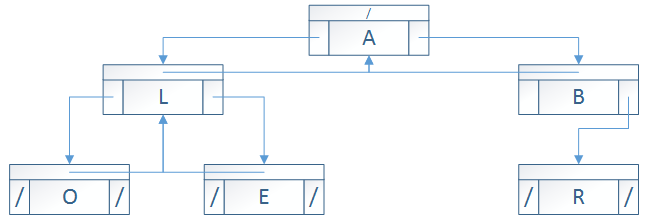
\includegraphics[width=0.7\linewidth]{images/albero_left_right_children}
\end{center}
\begin{lstlisting}[language=c,mathescape=true]
// T(n) = Theta(1)
padre(Tree t, Nodo v)
	return v.p;

// T(n) = Theta(1)
figli(Tree t, Node v)
	l = creaLista();
	if(v.left != null)
		inserisci(v.left, l);
	if(v.right != null)
		inserisci(v.right, l);
	return l;
\end{lstlisting}
Se il numero di figli non è noto a priori, è possibile associare a ciascun nodo una lista di puntatori ai suoi figli, con un conseguente spreco di memoria. Per ovviare a questi problemi, la rappresentazione più adeguata per rappresentare un albero è la \textbf{rappresentazione binarizzata}.
\pagebreak
\subsection{Rappresentazione binarizzata}
In questa rappresentazione ogni nodo ha un puntatore al padre, uno al figlio più a sinistra e uno al fratello a destra:
\begin{itemize}[itemsep=0pt]
	\item \textit{x.key} = contenuto informativo
	\item \textit{x.p} = puntatore al padre
	\item \textit{x.left-child} = puntatore al figlio più a sinistra del nodo $x$
	\item \textit{x.right-sibling} = puntatore al fratello di $x$ immediatamente a destra
\end{itemize}
Questa rappresentazione costa $\varTheta(n)$ in memoria.
\begin{center}
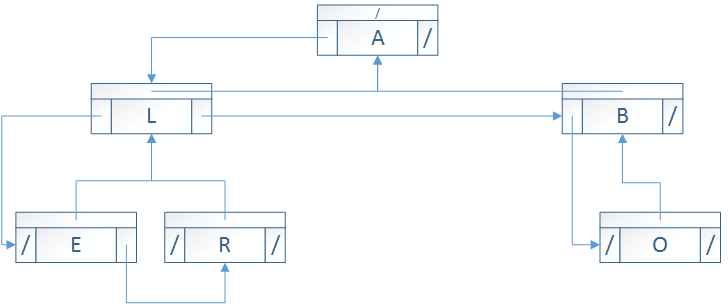
\includegraphics[width=0.7\linewidth]{images/albero_lista_figlio_sinistro_Fratello_destro}
\end{center}
\begin{lstlisting}[language=c,mathescape=true]
// T(n) = Theta(grado(v)) = O(n)
figli(Tree t, Node v)
	l = creaLista();
	iter = v.left-child;
		while(iter != null)
		inserisci(iter, l),
		iter = iter.right-sibling;
	return l;
\end{lstlisting}
\pagebreak
\subsection{Visite di alberi}
Una visita generica di un albero si esegue nel seguente modo:
\begin{lstlisting}[language=c,mathescape=true]
visitaGenerica(Node r)
	S = {r}
	while(S != $\varnothing$)
		estrai un nodo u da S
		visita(u);
		S = S $\cup$ {figli di u}
\end{lstlisting}
\textbf{Teorema}: l’algoritmo di visita, applicato alla radice di un albero con $n$ nodi termina in $\varOmicron(n)$ iterazioni. Lo spazio usato per memorizzare S è $\varOmicron(n)$. La nostra ipotesi é che l'inserimento/cancellazione siano eseguiti in $\varTheta(n)$. \\\\
Ogni nodo verrà inserito ed estratto da $S$ una sola volta perché in un albero non si può tornare ad un nodo a partire dai suoi figli procedendo di figlio in figlio. Quindi le iterazioni del ciclo while saranno al più $\varOmicron(n)$. Poiché ogni nodo compare al più una volta nella mia struttura $S$, lo spazio richiesto è $\varOmicron(n)$.
\subsubsection{Visita in profondità}
\paragraph{Versione iterativa} per alberi binari (nodi con proprietà \textit{left} e \textit{right})
\begin{lstlisting}[language=c,mathescape=true]
// T(n) = lineare = Theta(n)
// DepthFirstSearch 
visitaDFS(Node r)
	Stack S
	Push(S,r);
	while(!stackEmpty(S))
		u = pop(S);
		if(u != null)
			visita(u);
			push(S,u.right);
			push(S,u.left);
\end{lstlisting}
\paragraph{Versione ricorsiva} per alberi binari (nodi con proprietà \textit{left} e \textit{right})
\begin{lstlisting}[language=c,mathescape=true]
// T(n) = lineare = Theta(n)
visitaDFSric(Node r)
	if(r != null) // albero non vuoto
		visita r;
		visitaDFSric(r.left);
		visitaDFSric(r.right);		
\end{lstlisting}
\subsubsection{Visita in ampiezza o a livelli}
\begin{lstlisting}[language=c,mathescape=true]
// BreadthFirstSearch (BFS). Visita a livelli
visitaBFS(Node r)
	Queue q;
	enqueue(q, r);
	while(!queueEmpty(q))
		u = dequeue(q);
		if(u != null)
			visit(u);
			enqueue(q,u.left);
			enuqeue(q,u.right);
\end{lstlisting}
\subsubsection{Tipi di visita}
A seconda della posizione dell'operazione di visita del nodo abbiamo 3 tipi di visita diversi:
\begin{center}
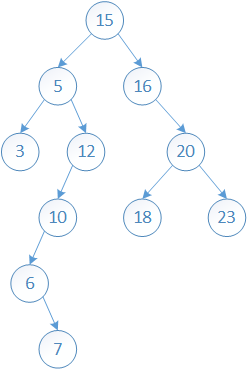
\includegraphics[width=0.2\linewidth]{images/albero_binario_esempio}
\end{center}
\begin{enumerate}
	\item Visita in \textbf{preordine}: si visita prima la radice, poi si effettuano le chiamate ricorsive prima sul figlio sinistro e poi sul destro. Nel caso dell'albero in esempio il risultato sarebbe: $\langle 1,2,4,5,6,3 \rangle$.
	\begin{lstlisting}[language=c,mathescape=true]
		visita r;
		visitaDFSric(r.left);
		visitaDFSric(r.right);
	\end{lstlisting}
	\item Visita \textbf{simmetrica}: si visita il figlio sinistro, la radice e il figlio destro: $\langle 4,2,6,5,1,3 \rangle$.
		\begin{lstlisting}[language=c,mathescape=true]
		visitaDFSric(r.left);
		visita r;
		visitaDFSric(r.right);
		\end{lstlisting}
	\item Visita in \textbf{post-ordine}: si visita il figlio sinistro, il figlio destro e la radice: $\langle 4,6,5,2,3,1 \rangle$.
		\begin{lstlisting}[language=c,mathescape=true]
		visitaDFSric(r.left);
		visitaDFSric(r.right);
		visita r;
		\end{lstlisting}
\end{enumerate}
Tutte queste visite hanno complessità uguale a $\varTheta(n)$.
\pagebreak
\subsubsection{Teorema}
Se $x$ è la radice di un sottoalbero di $n$ nodi, la chiamata \textit{visitaDFSric}, applicata al nodo $x$, richiede tempo $\varTheta(n)$.
\paragraph{Dimostrazione} Sia $T(n)$ il tempo richiesto dalla procedura quando è chiamata sulla radice di un sottoalbero di $n$ nodi. Poiché \textit{visitaDFSric} visita \underline{tutti} gli $n$ nodi del sottoalbero su cui è invocata, questa proprietà rappresenta un limite inferiore sotto al quale la complessità non può andare, quindi $T(n) = \varOmega(n)$. \\\\
Ora devo trovare il limite superiore, che ipotizzo essere $\varOmicron(n)$. Assumo che il sottoalbero sinistro abbia $k$ nodi, con $k<n$, e il sottoalbero destro $\underbracket{n}_{\mathclap{\text{tutti i nodi}}}-k-\overbracket{1}^{\mathclap{\text{radice}}}$ nodi, quindi:
\[
	T(n) = 
	\begin{cases*}
		\text{costante } c \qquad\qquad \text{se } n=0 \\
		\underbracket{T(k)}_{\mathclap{\text{sottoalbero sinistro}}} + \overbracket{T(n-k-1)}^{\mathclap{\text{sottoalbero destro}}} + d \qquad \text{se } n>0
	\end{cases*}
\]
Devo dimostrare che 
\[
	T(n) = an + b
\]
è una soluzione della ricorrenza $T(k) + T(n-k-1) + d$. Per induzione, il caso base è $n=0$:
\[
	T(0) = a\cdot 0 + b = b
\]
suppongo
\[
	b=c
\] 
e formulo l'ipotesi induttiva: assumiamo vero che per tutti gli $ m < n$, $T(n)=am+b$, e lo dimostro per $n$ (con $n>0$):
\[
	T(k) + T(n-k-1) + d
\]
applico l'ipotesi induttiva in quanto $k<n$ (non c'è la radice) e $n-k-1 < n$
\[
	ak+b+a(n-k-1)+b+d = a(\cancel{k}+n-\cancel{k}-1) + 2b + d = an-a+2b+d
\]
che devo imporre uguale a $an+b$, quindi
\[
	\cancel{an}-a+2b+d = \cancel{an}+b
\]
da cui
\[
	a=b+d
\]
ma avendo imposto $b=c$ all'inizio ottengo
\[
	a=c+d
\]
Quindi 
\[
	T(n) = an+b = (\underbracket{c+d}_{\mathclap{a}})\cdot n + \underbracket{b}_{\mathclap{b=c}}
\]
che è esattamente la funzione lineare della nostra occorrenza.
\subsection{Esercizi}
\subsubsection{\exercize - verificare completezza albero binario}
Dato un albero, scrivere una funzione che ritorna \textit{true} se l'albero è binario completo, \textit{false} altrimenti e ritorni inoltre l'altezza dell'albero stesso. La firma della funzione è la seguente:
\begin{lstlisting}[language=c,mathescape=true]
	verificaCompleto(Node u) : <bool,int>
\end{lstlisting}
Un albero binario completo ha due proprietà:
\begin{enumerate}[itemsep=0pt]
	\item ogni nodo interno ha $n$ figli
	\item tutte le foglie sono allo stesso livello
\end{enumerate}
L'implementazione diventa quindi:
\begin{lstlisting}[language=c,mathescape=true]
	verificaCompleto(Node u)
		if(u == null)
			return <true, -1>; // -1 = albero vuoto, 0 = solo radice
		<completoSx, hSx> = verificaCompleto(u.left);
		<completoDx, hDx> = verificaCompleto(u.right);
		// verifico siano completi e abbiano stesso livello
		completo = completoSx && completoDx && (hSx == hDx); 
		// possono avere altezze diverse a cui devo aggiungere la radice
		h = max(hSx,hDx) + 1;
		return <completo, h>;
\end{lstlisting}
La complessità è
\[
	T(n) = 
	\begin{cases*}
		c \qquad\text{se } n=0 \\
		T(k) + T(n-k-1) + d \qquad\text{se } n>0 
	\end{cases*}
\]
che equivale ad $\varTheta(n)$.
\pagebreak
\subsubsection{\exercize - numero di nodi intermedi}
Un nodo $u$ di un albero binario si dice \textit{intermedio} se la somma delle chiavi nei sottoaberi contenuti nei nodi del sottoalbero di cui $u$ è radice, è uguale alla somma delle chiavi contenute nei nodi sul percorso che collega il nodo $u$ alla radice, e da questo percorso $u$ deve essere escluso.
\begin{center}
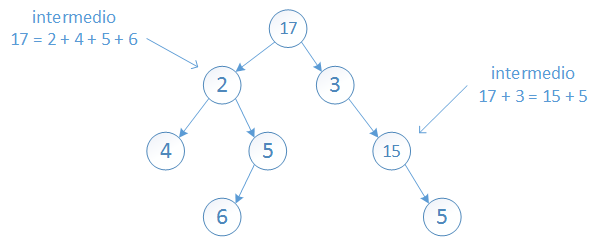
\includegraphics[width=0.7\linewidth]{images/nodi_intermedi}
\end{center}
Definito il tipo \textit{Node} nel seguente modo:
\begin{lstlisting}[language=c,mathescape=true]
	typedef struct node {
		int key,
		struct node* left,
		struct node* right
	} *Node;
\end{lstlisting}
si definisca la funzione che determini il numero di nodi intermedi di un albero:
\begin{lstlisting}[language=c,mathescape=true]
	int intermedi(Node u, int sum, int* sommaChiavi){
		int risSx, risDx, sommaChiaviSx, sommaChiaviDx;
		if(u == null){
			*sommaChiavi = 0;
			return 0;
		}
		risSx = intermedi(u.left, sum + u.key, &sommaChiviSx);
		risDx = intermedi(u.right, sum + u.key, &sommaChiviDx);
		*sommaChiavi = sommaChiviSx + sommaChiaviDx + u.key;
		if(sommaChiavi == sum)
			return 1 + risSx + risDx;
		else
			return risSx + risDx;
	}
\end{lstlisting}
La complessità risulta essere 
\[
	T(n) = 
	\begin{cases*}
		c \qquad\text{se } n=0 \\
		T(k) + T(n-k-1) + d \qquad\text{se } n>0 
	\end{cases*}
	\qquad = \varTheta(n)
\]
\pagebreak
\subsection{Alberi bilanciati}
Un albero è bilanciato se
\[
	h = O(\log n)
\]
Un albero binario completo è sempre bilanciato (in quanto completo). Viceversa un albero bilanciato non implica sia completo.
\subsubsection{\exercize: Costruire ricorsivamente un albero bilanciato}
Dato un array $v$ di $n$ interi, scrivere una funzione efficiente che costruisca ricorsivamente un albero binario bilanciato tale che $v[i]$ sia l'$(i+1)$-esimo campo $v.key$ in ordine di visita posticipata (\textit{postordine}). La firma della funzione è la seguente:
\begin{lstlisting}[language=c,mathescape=true]
	Node costruisci(int v[], int dim);
\end{lstlisting}
Per scrivere questa funzione abbiamo bisogno di alcuni parametri che non abbiamo in questa firma. Andiamo quindi a definire una nuova funzione:
\begin{lstlisting}[language=c,mathescape=true]
	Node costruisciAux(int v[], Node padre, int inf, int sup){
		Node r;
		int med;
		if(inf > sup)
			return null;
		else{
			r = malloc(sizeof(struct node));
			r->key = v[sup];
			r->p = padre;
			med = (inf+sup)/2;
			r->left = costruisciAux(v,r,inf,med-1);
			r->right = costruisciAux(v,r,med,sup-1);
			return r;
		}
	}
\end{lstlisting}
arrivati a questo punto richiamo la funzione iniziale:
\begin{lstlisting}[language=c,mathescape=true]
	Node costruisci(int v[], int dim){
		return costruisciAux(v,null,0,dim-1);
	}
\end{lstlisting}
La complessità risulta essere 
\[
	T(n) = 
	\begin{cases*}
		c \qquad\text{se } n=0 \\
		2T(\frac{n}{2}) + d \qquad\text{se } n>0 
	\end{cases*}
\]
risolvo con il teorema master:
\begin{gather*}
	n^{\log_ab} = n^{\log_22} = n \\
	\fn = d = \varTheta(1) \Rightarrow \text{1° caso del teorema} \\
	\fn = O(n^{1-\varepsilon}) \text{ con } \varepsilon > 0
\end{gather*}
pongo $\varepsilon = 1$ da cui ricavo 
\[
	T(n) = \varTheta(n)
\]

\subsubsection{\exercize: Stampare le chiavi di un livello $k$}
Dato un albero binario $T$ e un intero $k\geq0$, stampare le chiavi contenute in $T$ a livello $k$ procedendo da sinistra a destra.
\begin{lstlisting}[language=c,mathescape=true]
	void stampaLivello(Node v, int k){
		if(u == null)
			return;
		else{
			if(k == 0)
				printf("%d ", v.key);
			else{
				stampaLivello(v.left, k-1);
				stampaLivello(v.right, k-1);
			}
		}
	}
\end{lstlisting}
La complessità è $O(n)$, dove $n$ è il numero di nodi dell'albero, poiché il caso peggiore risulta essere $k = h(T)$. Se volessimo invece esprimere la complessità in funzione di $k$ il caso peggiore risulta essere quando $T$ è completo. In questo caso la complessità (sempre in funzione di $k$) risulta essere:
\[
	\sum_{i=0}^{k}2^i = \dfrac{2^{k+1}-1}{2-1} \approx 2^k 
\]
ovvero esponenziale.

\subsubsection{\exercize: Dimezzare le chiavi sui livelli pari di un albero}
Sia $T$ un albero generale i cui nodi hanno chiavi intere e proprietà \textit{key, left-child, right-sib}. Scrivere una funzione ricorsiva che trasforma $T$ dimezzando i valori di tutte le chiavi sui livelli pari dell'albero.
\begin{lstlisting}[language=c,mathescape=true]
	void trasforma(Node u){
		if(u != null) {
			u.key = u.key / 2;
			trasforma(u.right-sib);
			iter = u.left-child;
			while(iter){
				trasforma(iter.left-child);
				iter = iter-right-sib;
			}
		}
	}
\end{lstlisting}
La complessità risulta essere $O(n)$.
\pagebreak
\subsection{Alberi binari di ricerca}
Un albero binario di ricerca è un albero binario che soddisfa la seguenti proprietà:
\begin{enumerate}[label=\alph*)]
	\item Sia $x$ un nodo in un albero binario di ricerca. Se $y$ è un nodo nel sottoalbero sinistro di $x$, allora $y.key \leq x.key$
	\item Se $y$ è un nodo del sottoalbero destro di $x$, allora $y.key \geq x.key$
\end{enumerate}
La proprietà di ricerca dell'albero binario di ricerca consente di elencare in ordine crescente le chiavi del''albero stesso, visitandolo in ordine simmetrico.

\paragraph{\homeExercize}
Dimostrare per induzione sul numero di nodi dell'albero che le chiavi sono ordinate in modo crescente. 

\subsubsection{Operazioni}
Le operazioni definite su un albero binario di ricerca sono:
\begin{enumerate}[label=\alph*),itemsep=0pt]
	\item \textit{treeSearch}
	\item \textit{treeMinumum}
	\item \textit{treeSuccessor}
	\item \textit{treeInsert}
	\item \textit{treeDelete}
\end{enumerate}
\paragraph{a) \textit{treeSearch}} Ricerca un nodo con chiave $k$:
\begin{lstlisting}[language=c,mathescape=true]
	// post: restituisce un nodo con chiave $k$ se esiste, null altrimenti
	// complessità: O(T(h)), ovvero O(altezza albero)
	Node treeSearch(Node x, Elem k)
		if(x == null || x.key == k)
			return x;
		else
			if(x.key < k)
				return treeSearch(x.left, k);
			else
				return treeSearch(x.right, k);
\end{lstlisting}
I nodi incontrati durante la ricorsione formano un cammino verso il basso dalla radice dell'albero, quindi il tempo di esecuzione è $O(h(T))$. Se l'albero è bilanciato allora $T(n) = O(\log n)$. Se l'albero è fortemente sbilanciato allora $T(n) = O(n)$. \\\\
Esiste anche una versione iterativa del \textit{treeSearch}:
\begin{lstlisting}[language=c,mathescape=true]
	// post: restituisce un nodo con chiave $k$ se esiste, null altrimenti
	Node treeSearch(Node x, Elem k)
		while(x != null && x.key != k){
			if(x.key > k)
				x = x.left;
			else
				x = x.right;
		}
		return x;
\end{lstlisting}
\paragraph{b) \textit{treeMinumum}} Ricerca il nodo con chiave minore nel sottoalbero più in basso a sinistra.
\begin{lstlisting}[language=c,mathescape=true]
	// pre: x $\in$ T
	// post: restituisce il nodo con chiave minore nel sottoalbero radicato in $x$
	// complessità: O(n)
	Node treeMinimum(Node x){
		while(x != null)
			x = x.left;
		return x;
	}
\end{lstlisting}
\paragraph{c) \textit{treeSucessor}} Dato un nodo $n$ in un albero binario di ricerca, il successore di $x$ è il nodo che segue $x$ nell'ordine stabilito da una visita simmetrica. Se tutte le chiavi sono distinte il successore di un nodo $x$ è il nodo con la più piccola chiave maggiore di quella di $x$. Si distinguono due casi:
\begin{enumerate}[itemsep=0pt,label=\arabic*)]
	\item $x$ ha un figlio destro: il successore di $x$ è il minimo del sottoalbero destro di x
	\item $x$ non ha un figlio destro: il successore di $x$, se esiste, è l'antenato più prossimo di $x$ il cui figlio sinistro è anche antenato di $x$. Per trovarlo si risale da $x$ verso la radice, fino ad incontrare la "prima svolta a destra"
\end{enumerate}

\begin{lstlisting}[language=c,mathescape=true]
	// complessità: O(h(T))
	treeSuccessor(Node x){
		if(x.right != null)
			return treeMinumum(x.right); // O(h)
		else{
			y = x.p;
			while(y != null && x == y.right){ // O(h)
				x = y;
				y = y.p;
			}
			return y;
		}
	}
\end{lstlisting}
\paragraph{d) \textit{treeInsert}} \textit{Tree} è il tipo albero e ha un campo \textit{root} che contiene il nodo radice. Il nodo $z$ da inserire è inizializzato con la chiave e $z.left = z.right = null$
\begin{lstlisting}[language=c,mathescape=true]
	// complessità: O(h(T))
	treeInsert(Tree t, Node z){
		y = null;
		x = t.root;
		while(x != null){
			y = x;
			if(z.key < x.key)
				x = x.left;
			else
				x = x.right;
		}
		z.p = y;
		if(y == null)
			t.root = z;
		else
			if(z.key < y.key)
				y.left = z;
			else
				y.right = z;
	}
\end{lstlisting}

\paragraph{e) \textit{treeDelete}} elimina il nodo $z$ contenuto nell'albero $t$. Si distinguono 3 casi:
\begin{enumerate}[itemsep=0pt,label=\arabic*)]
	\item Se $z$ non ha figli, modifichiamo il padre di $z$ affinché punti anziche a $z$ a \textit{NULL}.
	\item Se $z$ ha un unico figlio, stacchiamo $z$ creando un collegamento tra il padre e il figlio di $z$.
	\item Se $z$ ha due figli, troviamo il successore $y$ di $z$, che si troverà nel sottoalbero destro di $z$, e facciamo in modo che $y$ assuma la posizione di $z$ nell'albero.
\end{enumerate}
Per realizzare questa funzione utilizzeremo una procedura ausiliaria \textit{trasplant} che, dato un albero $t$ e due nodi $u$ e $v$, sostituisce il sottoalbero con radice $u$ con il sottoalbero di radice $v$.
\begin{lstlisting}[language=c,mathescape=true]
// complessità: $\varTheta(1)$
transplant(Tree t, Node u, Node v){
	if(u.p == NULL) // il vecchio nodo è radice
		t.root = v; 
	else if(u == u.p.left) // il vecchio nodo è figlio sx
		u.p.left = v;
	else // il vecchio nodo è figlio destro
		u.p.right ) v;
	if(v != NULL) // se è un nodo
		v.p = u.p;
}
\end{lstlisting}
Ora possiamo andare ed implementare \textit{treeDelete}:
\begin{lstlisting}[language=c,mathescape=true]
// complessità: O(h)
treeDelete(Tree t, Node z){
	if(z.left == NULL)
		transplant(t, z, z.right);
	else if(z.right == NULL)
		transplant(t, z, z.left);
	else {
		y = treeMinimum(z.right); // O(h)
		if(y.p != z) {
			transplant(t, y, r.right);
			y.right = z.right;
			z.right.p = y;
		}
		transplant(t, z, y);
		y.left = z.left;
		y.left.p = y;
	}
}
\end{lstlisting}
\pagebreak
\subsubsection{\exercize: dimostrazione}
Dimostrare che se un nodo in un albero binario di ricerca ha due figli, allora il suo successore non ha un figlio sinistro e il suo predecessore non ha un figlio destro.
\begin{center}
	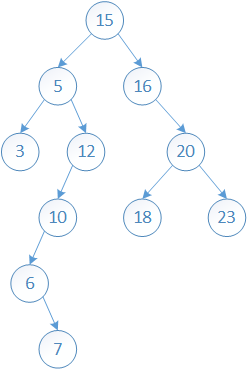
\includegraphics[width=0.3\linewidth]{images/albero_binario_esempio}
\end{center}
Se prendiamo in considerazione il nodo $5$, dobbiamo quindi dimostrare che il nodo $6$ suo successore non ha un figlio sinistro e che il nodo $3$ suo predecessore non ha un figlio destro. \\\\
Sia $x$ un nodo con due figli. In una visita simmetrica i nodi del sottoalbero sinistro precedono $x$ e quelli del sottoalbero destro lo seguono. Così il predecessore di $x$ si troverà nel sottoalbero sinistro di $x$, mentre il successore di $x$, se esiste, si troverà nel sottoalbero destro di $x$ stesso. \\\\
Sia $s$ il successore di $x$. Assumiamo per assurdo (per arrivare ad una contraddizione) che $s$ abbia un figlio sinistro $y$. Se così fosse $y$ seguirebbe $x$ nella visita perché si trova nel sottoalbero destro di $x$, ma precede $s$ perché è nel sottoalbero sinistro di $s$. Dunque l'ordine della visita sarebbe:
\[
	x \to y \to s
\]
Assurdo perché $s$ non sarebbe il successore di $x$ se avesse un figlio sinistro. In modo simmetrico si può dimostrare che il successore di $x$ non ha un figlio destro.

\subsubsection{Teorema}
Le operazioni quali \textit{search, treeMinimum, treeMaximum, successor, predecessor, insert e delete} sugli insiemi dinamici, possono essere svolte in tempo $\varOmicron(h)$ usando un albero di ricerca binario di altezza $h$. L'unico nodo per mantenere queste operazioni efficienti è tenere l'albero bilanciato, in modo che esse siano svolte in tempo $\varOmicron(\log n)$ dove $n$ è il numero dei nodi (in un albero bilanciato infatti $h = \log n$).

\pagebreak
\subsection{Alberi AVL}
Gli alberi AVL (Adelson-Velskij e Landis) sono alberi binari di ricerca bilanciati. Oltre alla chiave mantengono un informazione sul blianciamento. Il fattore di bilanciamento di un nodo è la differenza tra l'altezza del sottoalbero sinistro e quello destro. In un albero AVL il fattore di bilanciamento è sempre minore o uguale a 1 in ogni nodo.

\subsection{B-Alberi}
Sono degli alberi di ricerca bilanciati di grado minimo $t$, con $t \geq 2$, con le seguenti caratteristiche:
\begin{enumerate}[itemsep=0pt,label=\arabic*)]
	\item Tutte le foglie sono allo stesso livello, ovvero hanno stessa profondità.
	\item Ogni nodo $v$ diverso dalla radice mantiene un numero di chiavi $k(v)$ ordinate e $k_1(v) \leq k_2(v) \leq \dots \leq k(v)$ tale che $t-1 \leq k(v) \leq 2t-1$.
	\item La radice mantiene almeno una chiave ed al più $2t-1$ chiavi ordinate.
	\item Ogni nodo interno $v$ ha $k(v)+1$ figli.
	\item Le chiavi presenti nei figli $k_i(v)$ separano gli intervalli di chiavi memorizzate in ciascun sottoalbero: se $c_1$ è una qualunque chiave nel i-esimo sottoalbero di un nodo $v$ allora $c_1 \leq k_1(v) \leq c_2 \leq k_2(v) \dots$
\end{enumerate}
\begin{center}
	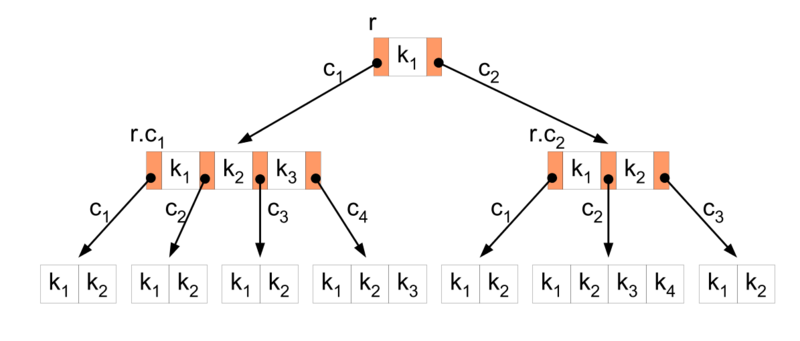
\includegraphics[width=0.7\linewidth]{images/b_tree}
\end{center}
\pagebreak

\section{Algoritmi di Ordinamento}
Il problema dell’ordinamento è che dato in input una sequenza di $n$ numeri $\langle a_1,a_2,\dots, a_n \rangle$ si vuole produrre in output una permutazione della sequenza di input $\langle a_1,a_2,\dots, a_n \rangle$ tale che
$\langle a_1 \leq a_2 \leq \dots \leq a_n \rangle$. \\\\
Per la soluzione di questo problema vi sono differenti approcci ed algoritmi.
\subsection{Algoritmi basati sul confronto}
\subsubsection{InsertionSort}
Algoritmo basato sulla tecnica incrementale: se ho $k$ elementi già ordinati estendo la mia soluzione al k+1-esimo elemento.\\\\
Questo algoritmo può essere paragonato all'ordinamento che eseguiamo quando riceviamo delle carte: la parte ordinata è la parte che teniamo in mano, l’altra sono le carte che dobbiamo ancora ricevere.
\begin{lstlisting}[language=c,mathescape=true]
	InsertionSort(Array a) {
		for(j=2 to a.length) {
			key = a[j]
			i = j-1;    
			while(i > 0 AND key < a[i]) {
				a[i+1] = a[i];
				i = i - 1;
			}
			A[i+1] = key;
		}
	}
\end{lstlisting}
Questo algoritmo presenta alcune peculiarità, ad esempio l'\textit{ordinamento in loco}.
\paragraph{Ordinamento in loco}: un algoritmo ordina sul posto se in ogni istante al più un numero costante di elementi dell’array di input sono memorizzati all’esterno dell’array.

\paragraph{Dimostrazione di correttezza}
Per dimostrare che questo algoritmo è corretto, dobbiamo trovare gli invarianti.

\paragraph{Invariante del ciclo esterno} Il sotto-array $a[1,..., j-1]$ è formato dagli elementi ordinati che originariamente erano nella posizione $a[1,..., j-1]$. 
\subparagraph{\homeExercize} Dimostrare che questo sia un invariante.

\paragraph{Teorema} l’algoritmo \textit{insertionSort} ordina in loco $n$ elementi eseguendo nel caso peggiore (input decrescente) $\varTheta(n^2)$ confronti. Il ciclo esterno è eseguito $(n-1)$ volte e il numero totale di confronti è:
\[
	\sum_{j=2}^{n} (j-1) = \sum_{k=1}^{n-1} k = \dfrac{(n-1+1)(n-1)}{2} = \dfrac{n(n-1)}{2} = \varTheta(n^2)
\]
Questo algoritmo è sensibile all’ordinamento degli elementi in input. Viene tuttavia utilizzato spesso in vettori di piccole dimensioni.

\pagebreak
\subsubsection{MergeSort}
Algoritmo di ordinamento basato sulla tecnica del \textit{divide te impera}. Si vuole ordinare un vettore $a[p,\dots,r]$ inizialmente $p=1$ e $r=n=a.length$. I passi da svolgere sono:
\begin{enumerate}[itemsep=0pt,label=\arabic*)]
	\item \textit{[divide]} si divide l’array in due sotto-array $a[p,\dots,q]$ e $a[q+1,\dots,r]$ con $q = \lfloor \frac{p+r}{2}\rfloor$.
	\item \textit{[impera]} si ordinano i due sotto-array in modo ricorsivo utilizzando \textit{mergeSort}. Se il problema è sufficientemente piccolo risolve direttamente.
	\item \textit{[ricomponi]} si fondono insieme i due sotto-array ordinati per generare un singolo vettore ordinato $a[p,\dots,r]$.
\end{enumerate}
\begin{lstlisting}[language=c,mathescape=true]
	mergeSort(Array a, int p, int r){
		if(p<r){
			q = $\lfloor$(p+r)/2$\rfloor$; // parte intera
			mergeSort(a,p,q);
			mergeSort(a,q+1,r);
			merge(a,p,q,r);
		}else{
			// p==r --> 1 elemento
			// p > r --> 0 elementi
			// caso base
			// non faccio nulla
		}
	}
\end{lstlisting}
La procedura \textit{merge}: $p \leq q < r$. Il sotto-array $a[p,\dots,q]$ è ordinato e anche il sotto-array $a[q+1,\dots,r]$ è ordinato. Per le restrizioni che abbiamo sui parametri $p$, $q$ ed $r$ sappiamo che nessuno degli sotto-array è vuoto. L’output della funzione è la fusione dei due sotto-array in un unico array ordinato $a[p,\dots,r]$.
\begin{lstlisting}[language=c,mathescape=true]
	merge(Array a, int p, int q, int r){
		int n1 = q-p+1; // numero elementi a sinistra
		int n2 = r-q; // numero di elementi a destra
		crea array l di dimensione n1+1;
		crea array r di dimensione n2+1;	
		for(i=0 to n1)
			l[i] = a[p+i-1];
		for(i=0 to n2)
			r[i] = a[q+i];
		l[n1+1] = $\infty$; // guardia per evitare controlli sui bounds
		r[n2+1] = $\infty$; // guardia per evitare controlli sui bounds
		i = 1; // indice per l
		j = 1; // indice per r
		for(k=p to r){
			if(l[i] <= r[j]) {
				a[k] = l[i];
				i++;
			}
			else { 
				a[k] = l[j];
				j++;
			}
		}
	}
\end{lstlisting}
Invariante: il sotto-array $a[p,\dots,k-1]$ contiene ordinati gli $(k-p)$ elementi più piccoli presenti in  $l[1,\dots,n1+1]$ e $r[1,\dots,n2+1]$. Inoltre $l[i]$ e $r[j]$ sono i più piccoli elementi dei loro array che non sono stati copiati in $a$.
\end{document}
